%%% Lecture 1 Slides %%%

\documentclass{beamer}

%\documentclass[handout]{beamer}
%\usepackage{pgfpages}
%\pgfpagesuselayout{2 on 1}[a4paper,border shrink=5mm]
%\pgfpagesuselayout{1 on 1}[a4paper,border shrink=5mm]



\usepackage{amssymb}
\usepackage{amsmath}
\usepackage{mathtools}
\usepackage{tikz}
\usetikzlibrary{shapes,arrows}
\usetikzlibrary{positioning}
\usetikzlibrary{trees}
\usepackage{pgfplots}
\usepackage{pdflscape}
\usepackage{graphicx}
\usepackage{colortbl}
\usepackage{listings}
\usepackage{adjustbox}

\DeclarePairedDelimiter{\ceil}{\lceil}{\rceil}

\newcommand{\bs}{\boldsymbol}
\newcommand{\mb}{\mathbf}
\newcommand{\indep}{{\bot\negthickspace\negthickspace\bot}}
\newcommand{\notindep}{{\bot\negthickspace\negthickspace\bot}{\negthinspace
  \negmedspace \negthickspace \negthickspace \diagup
  \;}}
\renewcommand{\S}{\mb{S}}
\usepackage{color}
\definecolor{direct}{HTML}{FF0000}
\definecolor{indirect}{HTML}{FF9999}
\definecolor{dirin}{HTML}{990000}
\definecolor{control}{HTML}{999999}
\definecolor{directE}{HTML}{ED1C24}
\definecolor{indirectE}{HTML}{F69679}
\definecolor{controlE}{HTML}{999999}

%\defV{{\rm Var}\,}
\def\E{{\rm E}\,}
\def\arg{{\rm arg}\,}
\def\Cov{{\rm Cov}\,}
\def\N{{\rm N}\,}
\newcommand{\plim}{{\rm plim} \,}
\DeclareMathOperator*{\argmin}{arg\,min}
\newcommand{\X}{\mathbf{X}}
\newcommand{\Y}{\mathbf{Y}}
\newcommand{\Z}{\mathbf{Z}}
\newcommand{\I}{\mathbf{I}}
\newcommand{\V}{\mathbf{\Omega}}
\newcommand{\W}{\mathbf{W}}
\newcommand{\R}{\mathbf{R}}
\newcommand{\A}{\mathbf{A}}
\newcommand{\B}{\mathbf{B}}
\newcommand{\D}{\mathbf{D}}
\newcommand{\T}{\mathbf{T}}
\newcommand{\F}{\mathbf{F}}
\renewcommand{\O}{\mathbf{O}}
\renewcommand{\H}{\mathbf{H}}
\newcommand{\g}{\mathbf{g}}
\renewcommand{\r}{\mathbf{r}}
\newcommand{\s}{\mathbf{s}}
\newcommand{\uu}{\mathbf{u}}
\newcommand{\w}{\mathbf{w}}
\newcommand{\x}{\mathbf{x}}
\newcommand{\vv}{\mathbf{v}}
\newcommand{\z}{\mathbf{z}}
\newcommand{\y}{\mathbf{y}}

\newcommand{\bi}{\begin{itemize}}
\newcommand{\ei}{\end{itemize}}
\newcommand{\be}{\begin{enumerate}}
\newcommand{\ee}{\end{enumerate}}

\newcommand{\Beta}{\boldsymbol{\beta}}
\newcommand{\btheta}{\boldsymbol{\theta}}
\newcommand{\bgamma}{\boldsymbol{\gamma}}
\newcommand{\bpi}{\boldsymbol{\pi}}
\newcommand{\arrowp}{\stackrel{p}{\rightarrow}}
\newcommand{\arrowd}{\stackrel{d}{\rightarrow}}
\newcommand{\0}{\mathbf{0}}
\newcommand{\bP}{\mathbf{P}}
\newcommand{\nn}{\nonumber}
\def\S{{\sigma}}
\def\Supp{{\rm Supp}\,}


\newcommand\independent{\protect\mathpalette{\protect\independenT}{\perp}}
\def\independenT#1#2{\mathrel{\rlap{$#1#2$}\mkern2mu{#1#2}}}

\newcommand{\vsf}{\vspace{.5cm}}

\usepackage[english]{babel}
% or whatever

\usepackage[latin1]{inputenc}
% or whatever

\usepackage{times}
\usepackage[T1]{fontenc}
\setbeamertemplate{footline}[page number]{}
\setbeamertemplate{navigation symbols}{}


\title[QTM 220: AM slides] % (optional, use only with long paper titles)
{QTM 220: AM}

\subtitle{Aronow and Miller plus}

\author{Adam Glynn\\
\vspace{.5cm} \scriptsize
many slides, tex, and figures used with permission from Peter Aronow, Daniel Arnon, Elisha Cohen, Allison Cuttner, and Kevin Quinn}


%\AtBeginSection[]
%{
%  \begin{frame}<beamer>
%    \frametitle{Outline}
%    \tableofcontents[currentsection,currentsubsection]
%  \end{frame}
%}
%
%
%\AtBeginSubsection[]
%{
%  \begin{frame}<beamer>
%    \frametitle{Outline}
%    \tableofcontents[currentsection,currentsubsection]
%  \end{frame}
%}

\begin{document}

\begin{frame}
  \titlepage
\end{frame}

%\begin{frame}
%  \frametitle{Outline}
%  \tableofcontents
%\end{frame}

%\frame{
%
%Review of Summarizing Distributions: \\
%
%\vspace{0.2in}
%
%Expected values, [co]variances, conditional expectation functions, best [linear] predictors.
%
%}

\frame{

The expected value [expectation] of an R.V.: the average realization over hypothetical random draws.

\vspace{0.2in}

Discrete:
$$
\E[X] = \sum_{x \in \Supp(X)} x f(x)
$$

\vspace{0.2in}

Continuous:
$$
\E[X] = \int_{-\infty}^{\infty} x f(x) dx
$$

What does this mean, physically?

}

\frame{
\begin{center}
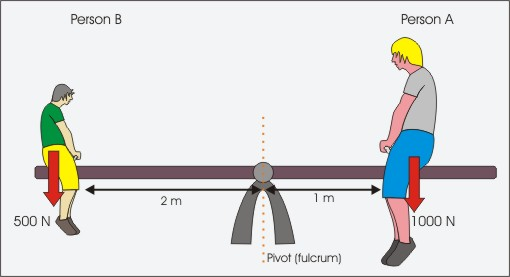
\includegraphics[scale=.5]{figures/seesaw}
\end{center}
}

\frame{
What do we mean by random draws?
\begin{table}[h]
\begin{center}
{\scriptsize
\begin{tabular}{r|r|r|r|r|r} %cc
$i$ & \multicolumn{1}{r|}{1} & \multicolumn{1}{r|}{2}   & $\dots$ & \multicolumn{1}{r|}{625} & \\ % & \multicolumn{1}{c}{$MoE$}& \multicolumn{1}{c}{95\% CI}  \\
$s$  & $Y_1$  & $Y_2$   & $\dots$  & $Y_{625}$  & $\overline{Y}_{625}$ \\ % & $2\cdot\sqrt{\frac{\overline{Y}_{625}(1-\overline{Y}_{625})}{625}}$ & $\overline{Y}_{625} \pm MoE$ \\
\hline
1 & 1 & 1   & $\dots$  & 0 & .68  \\ %& \visible<2->{.037} & \visible<3->{[.643,.717]}\\
2 & 0 & 1   & $\dots$  & 1 & .70 \\ %& \visible<2->{.037}  & \visible<3->{[.663,.737]}\\
3 & 0 & 0  & $\dots$  & 1 & .75 \\ %& \visible<2->{.035} & \visible<3->{[.715,.785]}\\
4 & 0 & 1 & $\dots$  & 1 & .73 \\ %& \visible<2->{.036} & \visible<3->{[.694,.766]}\\
5 & 0 & 1  & $\dots$  & 1 & .69 \\ %& \visible<2->{.037} & \visible<3->{[.653,.727]}\\
$\vdots$ & $\vdots$  & $\vdots$ & $\vdots$ & $\vdots$  & $\vdots$ \\ % & \visible<2->{$\vdots$} & \visible<3->{$\vdots$}  \\
1 mil  & 0 & 1& $\dots$  & 1 & .74 \\ %& \visible<2->{.035}& \visible<3->{[.705,.775]}\\
 $\vdots$  & $\vdots$  & $\vdots$ & $\vdots$ & $\vdots$  & $\vdots$ \\ % & \visible<2->{$\vdots$} & \visible<3->{$\vdots$}\\
\hline
\visible<1->{$f_{\cdot}(\cdot)$} & \multicolumn{1}{r|}{\visible<1->{Be(.71)}} & \multicolumn{1}{r|}{\visible<1->{Be(.71)}}  & & \multicolumn{1}{r|}{\visible<1->{Be(.71)}} & \visible<1->{$\frac{Bin(625,.71)}{625}$} \\
\visible<1->{$\E_{\cdot}(\cdot)$} & \multicolumn{1}{r|}{\visible<1->{.71}} & \multicolumn{1}{r|}{\visible<1->{.71}}  & & \multicolumn{1}{r|}{\visible<1->{.71}} & \visible<1->{$.71$} \\
\end{tabular}}
%\caption{\emph{Sampling Distributions for $\overline{Y}_{625}$, the Margin-of-Error, and the 95\% Confidence Interval}}\label{t:samdistCI}
\end{center}
\end{table}

}


\frame{
Beyond binary
\begin{table}[h]
\begin{center}
{\scriptsize
\begin{tabular}{r|r|r|r|r|r} %cc
$i$ & \multicolumn{1}{r|}{1} & \multicolumn{1}{r|}{2}   & $\dots$ & \multicolumn{1}{r|}{625} & \\ % & \multicolumn{1}{c}{$MoE$}& \multicolumn{1}{c}{95\% CI}  \\
$s$  & $Y_1$  & $Y_2$   & $\dots$  & $Y_{625}$  & $\overline{Y}_{625}$ \\ % & $2\cdot\sqrt{\frac{\overline{Y}_{625}(1-\overline{Y}_{625})}{625}}$ & $\overline{Y}_{625} \pm MoE$ \\
\hline
1 & 35 & 50   & $\dots$  & 22 & 45  \\ %& \visible<2->{.037} & \visible<3->{[.643,.717]}\\
2 & 28 & 19   & $\dots$  & 65 & 47 \\ %& \visible<2->{.037}  & \visible<3->{[.663,.737]}\\
3 & 33 & 27  & $\dots$  & 45 & 42 \\ %& \visible<2->{.035} & \visible<3->{[.715,.785]}\\
4 & $\vdots$ & $\vdots$ & $\dots$  & $\vdots$ & $\vdots$ \\ %& \visible<2->{.036} & \visible<3->{[.694,.766]}\\
5 & $\vdots$ & $\vdots$  & $\dots$  & $\vdots$ & $\vdots$ \\ %& \visible<2->{.037} & \visible<3->{[.653,.727]}\\
$\vdots$ & $\vdots$  & $\vdots$ & $\vdots$ & $\vdots$  & $\vdots$ \\ % & \visible<2->{$\vdots$} & \visible<3->{$\vdots$}  \\
1 mil  & 41 & 53& $\dots$  & 21 & 46 \\ %& \visible<2->{.035}& \visible<3->{[.705,.775]}\\
 $\vdots$  & $\vdots$  & $\vdots$ & $\vdots$ & $\vdots$  & $\vdots$ \\ % & \visible<2->{$\vdots$} & \visible<3->{$\vdots$}\\
\hline
\visible<1->{$f_{\cdot}(\cdot)$} & \multicolumn{1}{r|}{\visible<1->{?}} & \multicolumn{1}{r|}{\visible<1->{?}}  & & \multicolumn{1}{r|}{\visible<1->{?}} & \visible<1->{?} \\
\visible<1->{$\E_{\cdot}(\cdot)$} & \multicolumn{1}{r|}{\visible<1->{45}} & \multicolumn{1}{r|}{\visible<1->{45}}  & & \multicolumn{1}{r|}{\visible<1->{45}} & \visible<1->{?} \\
\end{tabular}}
%\caption{\emph{Sampling Distributions for $\overline{Y}_{625}$, the Margin-of-Error, and the 95\% Confidence Interval}}\label{t:samdistCI}
\end{center}
\end{table}

}



\frame{
Important properties:

$$
\E[c] = c
$$

$$
\E[aX] = a\E[X]
$$

\bigskip

Prove these assuming X is a discrete RV.
}






%\frame{
%
%Die roll:
%
%$$\E[X] = \sum_{x=1}^6 x f(x) =$$
%$$ 1 \times \frac{1}{6} + 2 \times \frac{1}{6} + 3 \times \frac{1}{6} + 4 \times \frac{1}{6} + 5 \times \frac{1}{6} + 6\times \frac{1}{6} = 3.5$$
%
%}

%\frame{
%
%Standard normal distribution:
%
%\begin{align*}
%\E[X] & = \int_{-\infty}^\infty x \frac{1}{\sqrt{2\pi}} e^{ -\frac{x^2}{2} } dx \\
%& = \frac{1}{\sqrt{2\pi}}  \int_{-\infty}^\infty x e^{ -\frac{x^2}{2} } dx \\
%& =  \frac{1}{\sqrt{2\pi}} -e^{ -\frac{x^2}{2} } \vert_{-\infty}^{\infty} \\
%& =  0.
%\end{align*}
%
%Hint: I don't care if you use Mathematica, Wolfram Alpha, or any other symbolic math solver.
%
%}



\frame{
Higher moments about the mean. The $j$th {\it central} moment:

$$
\mu_j = \E\left[ \left( X - \E[X] \right)^j \right].
$$



}

\frame{
The 2nd {\it central} moment, the variance:

\begin{align*}
V(X) &= \E\left[ \left( X - \E[X] \right)^2 \right] \\
 &= \visible<2>{\E\left[ X^2 - 2 X \E[X] +  \E[X]^2 \right]} \\
  &= \visible<2>{\E\left[ X^2\right] - 2 \E\left[ X \E[X] \right] +  \E\left[ \E[X]^2 \right]} \\
    &= \visible<2>{\E\left[ X^2\right] - 2  \E[X] \E[ X]  + \E[X]^2} \\
        &= \visible<2>{\E\left[ X^2\right] - 2  \E[X]^2  + \E[X]^2} \\
                &= \E\left[ X^2\right] -  \E[X]^2 \\
\end{align*}

\begin{itemize}
\item The average squared deviation from the expected value.
\item Expectation of the square minus the square of the expectation.
\end{itemize}

What does this mean, physically?
}

\frame{
\begin{center}
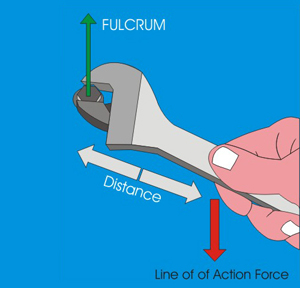
\includegraphics[scale=.5]{figures/turning_effect_01}
\end{center}
}

\frame{
What do we mean by random draws?
\begin{table}[h]
\begin{center}
{\scriptsize
\begin{tabular}{r|r|r|r|r|r} %cc
$i$ & \multicolumn{1}{r|}{1} & \multicolumn{1}{r|}{2}   & $\dots$ & \multicolumn{1}{r|}{625} & \\ % & \multicolumn{1}{c}{$MoE$}& \multicolumn{1}{c}{95\% CI}  \\
$s$  & $Y_1$  & $Y_2$   & $\dots$  & $Y_{625}$  & $\overline{Y}_{625}$ \\ % & $2\cdot\sqrt{\frac{\overline{Y}_{625}(1-\overline{Y}_{625})}{625}}$ & $\overline{Y}_{625} \pm MoE$ \\
\hline
1 & 1 & 1   & $\dots$  & 0 & .68  \\ %& \visible<2->{.037} & \visible<3->{[.643,.717]}\\
2 & 0 & 1   & $\dots$  & 1 & .70 \\ %& \visible<2->{.037}  & \visible<3->{[.663,.737]}\\
3 & 0 & 0  & $\dots$  & 1 & .75 \\ %& \visible<2->{.035} & \visible<3->{[.715,.785]}\\
4 & 0 & 1 & $\dots$  & 1 & .73 \\ %& \visible<2->{.036} & \visible<3->{[.694,.766]}\\
5 & 0 & 1  & $\dots$  & 1 & .69 \\ %& \visible<2->{.037} & \visible<3->{[.653,.727]}\\
$\vdots$ & $\vdots$  & $\vdots$ & $\vdots$ & $\vdots$  & $\vdots$ \\ % & \visible<2->{$\vdots$} & \visible<3->{$\vdots$}  \\
1 mil  & 0 & 1& $\dots$  & 1 & .74 \\ %& \visible<2->{.035}& \visible<3->{[.705,.775]}\\
 $\vdots$  & $\vdots$  & $\vdots$ & $\vdots$ & $\vdots$  & $\vdots$ \\ % & \visible<2->{$\vdots$} & \visible<3->{$\vdots$}\\
\hline
\visible<1->{$f_{\cdot}(\cdot)$} & \multicolumn{1}{r|}{\visible<1->{Be(.71)}} & \multicolumn{1}{r|}{\visible<1->{Be(.71)}}  & & \multicolumn{1}{r|}{\visible<1->{Be(.71)}} & \visible<1->{$\frac{Bin(625,.71)}{625}$} \\
\visible<1->{$\E_{\cdot}(\cdot)$} & \multicolumn{1}{r|}{\visible<1->{.71}} & \multicolumn{1}{r|}{\visible<1->{.71}}  & & \multicolumn{1}{r|}{\visible<1->{.71}} & \visible<1->{$.71$} \\
\visible<1->{$V_{\cdot}(\cdot)$} & \multicolumn{1}{r|}{\visible<1->{.71(1-.71)}} & \multicolumn{1}{r|}{\visible<1->{.71(1-.71)}}  & & \multicolumn{1}{r|}{\visible<1->{.71(1-.71)}} & \visible<1->{?} \\
\end{tabular}}
%\caption{\emph{Sampling Distributions for $\overline{Y}_{625}$, the Margin-of-Error, and the 95\% Confidence Interval}}\label{t:samdistCI}
\end{center}
\end{table}

}

\frame{
Beyond binary
\begin{table}[h]
\begin{center}
{\scriptsize
\begin{tabular}{r|r|r|r|r|r} %cc
$i$ & \multicolumn{1}{r|}{1} & \multicolumn{1}{r|}{2}   & $\dots$ & \multicolumn{1}{r|}{625} & \\ % & \multicolumn{1}{c}{$MoE$}& \multicolumn{1}{c}{95\% CI}  \\
$s$  & $Y_1$  & $Y_2$   & $\dots$  & $Y_{625}$  & $\overline{Y}_{625}$ \\ % & $2\cdot\sqrt{\frac{\overline{Y}_{625}(1-\overline{Y}_{625})}{625}}$ & $\overline{Y}_{625} \pm MoE$ \\
\hline
1 & 35 & 50   & $\dots$  & 22 & 45  \\ %& \visible<2->{.037} & \visible<3->{[.643,.717]}\\
2 & 28 & 19   & $\dots$  & 65 & 47 \\ %& \visible<2->{.037}  & \visible<3->{[.663,.737]}\\
3 & 33 & 27  & $\dots$  & 45 & 42 \\ %& \visible<2->{.035} & \visible<3->{[.715,.785]}\\
4 & $\vdots$ & $\vdots$ & $\dots$  & $\vdots$ & $\vdots$ \\ %& \visible<2->{.036} & \visible<3->{[.694,.766]}\\
5 & $\vdots$ & $\vdots$  & $\dots$  & $\vdots$ & $\vdots$ \\ %& \visible<2->{.037} & \visible<3->{[.653,.727]}\\
$\vdots$ & $\vdots$  & $\vdots$ & $\vdots$ & $\vdots$  & $\vdots$ \\ % & \visible<2->{$\vdots$} & \visible<3->{$\vdots$}  \\
1 mil  & 41 & 53& $\dots$  & 21 & 46 \\ %& \visible<2->{.035}& \visible<3->{[.705,.775]}\\
 $\vdots$  & $\vdots$  & $\vdots$ & $\vdots$ & $\vdots$  & $\vdots$ \\ % & \visible<2->{$\vdots$} & \visible<3->{$\vdots$}\\
\hline
\visible<1->{$f_{\cdot}(\cdot)$} & \multicolumn{1}{r|}{\visible<1->{?}} & \multicolumn{1}{r|}{\visible<1->{?}}  & & \multicolumn{1}{r|}{\visible<1->{?}} & \visible<1->{?} \\
\visible<1->{$V_{\cdot}(\cdot)$} & \multicolumn{1}{r|}{\visible<1->{25}} & \multicolumn{1}{r|}{\visible<1->{25}}  & & \multicolumn{1}{r|}{\visible<1->{25}} & \visible<1->{?} \\
\end{tabular}}
%\caption{\emph{Sampling Distributions for $\overline{Y}_{625}$, the Margin-of-Error, and the 95\% Confidence Interval}}\label{t:samdistCI}
\end{center}
\end{table}

}



\frame{
Important properties:

$$
V[c] = 0
$$

$$
V[aX] = a^2V[X]
$$

$$
V[c+ aX] = a^2V[X]
$$

\bigskip

Prove these assuming X is a discrete RV.
}

\frame{
What do these properties mean?
\begin{table}[h]
\begin{center}
{\scriptsize
\begin{tabular}{r|r|r|r|r|r} %cc
$i$ & \multicolumn{1}{r|}{1} & \multicolumn{1}{r|}{2}   & $\dots$ & \multicolumn{1}{r|}{625} & \\ % & \multicolumn{1}{c}{$MoE$}& \multicolumn{1}{c}{95\% CI}  \\
$s$  & $Y_1$  & $Y_2$   & $\dots$  & $Y_{625}$  & $\overline{Y}_{625}$ \\ % & $2\cdot\sqrt{\frac{\overline{Y}_{625}(1-\overline{Y}_{625})}{625}}$ & $\overline{Y}_{625} \pm MoE$ \\
\hline
1 & 1 & 1   & $\dots$  & 0 & .68  \\ %& \visible<2->{.037} & \visible<3->{[.643,.717]}\\
2 & 0 & 1   & $\dots$  & 1 & .70 \\ %& \visible<2->{.037}  & \visible<3->{[.663,.737]}\\
3 & 0 & 0  & $\dots$  & 1 & .75 \\ %& \visible<2->{.035} & \visible<3->{[.715,.785]}\\
4 & 0 & 1 & $\dots$  & 1 & .73 \\ %& \visible<2->{.036} & \visible<3->{[.694,.766]}\\
5 & 0 & 1  & $\dots$  & 1 & .69 \\ %& \visible<2->{.037} & \visible<3->{[.653,.727]}\\
$\vdots$ & $\vdots$  & $\vdots$ & $\vdots$ & $\vdots$  & $\vdots$ \\ % & \visible<2->{$\vdots$} & \visible<3->{$\vdots$}  \\
1 mil  & 0 & 1& $\dots$  & 1 & .74 \\ %& \visible<2->{.035}& \visible<3->{[.705,.775]}\\
 $\vdots$  & $\vdots$  & $\vdots$ & $\vdots$ & $\vdots$  & $\vdots$ \\ % & \visible<2->{$\vdots$} & \visible<3->{$\vdots$}\\
\hline
\visible<1->{$f_{\cdot}(\cdot)$} & \multicolumn{1}{r|}{\visible<1->{Be(.71)}} & \multicolumn{1}{r|}{\visible<1->{Be(.71)}}  & & \multicolumn{1}{r|}{\visible<1->{Be(.71)}} & \visible<1->{$\frac{Bin(625,.71)}{625}$} \\
\visible<1->{$\E_{\cdot}(\cdot)$} & \multicolumn{1}{r|}{\visible<1->{.71}} & \multicolumn{1}{r|}{\visible<1->{.71}}  & & \multicolumn{1}{r|}{\visible<1->{.71}} & \visible<1->{$.71$} \\
\visible<1->{$V_{\cdot}(\cdot)$} & \multicolumn{1}{r|}{\visible<1->{.71(1-.71)}} & \multicolumn{1}{r|}{\visible<1->{.71(1-.71)}}  & & \multicolumn{1}{r|}{\visible<1->{.71(1-.71)}} & \visible<1->{$\frac{625(.71)(1-.71)}{625^2}$} \\
\end{tabular}}
%\caption{\emph{Sampling Distributions for $\overline{Y}_{625}$, the Margin-of-Error, and the 95\% Confidence Interval}}\label{t:samdistCI}
\end{center}
\end{table}

}




\frame{
Definition:

\vspace{0.2in}


Standard deviation: $\sigma(X) = \sqrt{V(X)}$.

}

\frame{

Definition: mean squared error (MSE) about a guess $c$:
\begin{align*}
\E\left[(X - c)^2\right] &= \visible<2>{\E[X^2] - 2c\E[X] + c^2} \\
&= \visible<2>{\E[X^2] -\E[X]^2 + \E[X]^2 - 2c\E[X] + c^2} \\
&= V(X) + (\E[X] - c)^2
\end{align*}

\bigskip

 \visible<2>{What is the minimum MSE choice of c?}


}

%\frame{
%
%Definition: mean absolute error (MAE) about $c$:
%$$
%\E\left[|X - c|\right]
%$$
%
%What is the minimum MAE choice of c?\\
%%\vspace{.5cm}
%\vsf
%Hint: Remember your Hotelling/Downs.
%
%}




%\frame{
%
%A coinflip: heads (0), tails (1). What's the minimum MSE (MMSE) guess?
%
%$$
%f_{X}= \left\{
%     \begin{array}{lr}
%       1/2 & : x = 0 \\
%       1/2 & : x = 1
%            \end{array}
%   \right.
%$$
%
%\begin{align*}
%\E[ (X - c) ^2] &= 1/2 (0 - c)^2 + 1/2 (1 - c)^2 \\
%&= 1/2 \left[ c^2 + 1 +  c^2 - 2c\right] \\
%&= 1/2 \left[ 1 +  2c^2 - 2c\right]
%\end{align*}
%Could solve with FOC, but let's plot instead.
%}


%\frame{
%\begin{center}
%\includegraphics[width=.8\textwidth]{plot-mmse.PDF}
%\end{center}
%}

%\frame{
%
%So let's generalize all of these ideas to bi/multivariate relationships.
%
%}



\frame{
Defining expectation over a vector of RVs.
$$
\E[(X,Y)] = (\E[X],\E[Y])
$$
}

\frame{

Defining an expectation over functions multiple R.V.s.

\vspace{0.2in}

Let $Z = h(X,Y)$ be a scalar function of the random vector $(X,Y)$ as we proceed.

\vspace{0.2in}


Discrete:
$$
\E[Z] = \sum_{x \in \Supp(X)} \sum_{y \in \Supp(Y)} h(x,y) f(x,y)
$$

Continuous:
$$
\E[Z] = \int_{-\infty}^{\infty} \int_{-\infty}^{\infty} h(x,y) f(x,y) dy dx
$$

\vspace{0.2in}

So this is just a straightforward generalization (working with joint PMFs/PDFs).

}

\frame{
Important property:
Prove it for discrete.

\begin{align*}
\E[aX + bY+c] &= \visible<2>{\sum_{x \in \Supp(X)} \sum_{y \in \Supp(Y)} h(x,y) f(x,y)} \\
&= \visible<2>{\sum_{x \in \Supp(X)} \sum_{y \in \Supp(Y)} (ax + by+c) f(x,y)} \\
&= \visible<2>{\sum_{x \in \Supp(X)} \sum_{y \in \Supp(Y)} a \cdot x \cdot f(x,y)} \\
&+  \visible<2>{\sum_{x \in \Supp(X)} \sum_{y \in \Supp(Y)} b \cdot y \cdot f(x,y)+ c} \\
&= a\E[X] + b\E[Y] + c
\end{align*}



}


\frame{
What do these properties mean?
\begin{table}[h]
\begin{center}
{\scriptsize
\begin{tabular}{r|r|r|r|r|r} %cc
$i$ & \multicolumn{1}{r|}{1} & \multicolumn{1}{r|}{2}   & $\dots$ & \multicolumn{1}{r|}{625} & \\ % & \multicolumn{1}{c}{$MoE$}& \multicolumn{1}{c}{95\% CI}  \\
$s$  & $Y_1$  & $Y_2$   & $\dots$  & $Y_{625}$  & $\frac{1}{2}Y_1 + \frac{1}{2}Y_2$ \\ % & $2\cdot\sqrt{\frac{\overline{Y}_{625}(1-\overline{Y}_{625})}{625}}$ & $\overline{Y}_{625} \pm MoE$ \\
\hline
1 & 35 & 50   & $\dots$  & 22 & $\frac{1}{2}35 + \frac{1}{2}50$  \\ %& \visible<2->{.037} & \visible<3->{[.643,.717]}\\
2 & 28 & 19   & $\dots$  & 65 & $\frac{1}{2}28 + \frac{1}{2}19$ \\ %& \visible<2->{.037}  & \visible<3->{[.663,.737]}\\
3 & 33 & 27  & $\dots$  & 45 & $\frac{1}{2}33 + \frac{1}{2}27$ \\ %& \visible<2->{.035} & \visible<3->{[.715,.785]}\\
4 & $\vdots$ & $\vdots$ & $\dots$  & $\vdots$ & $\vdots$ \\ %& \visible<2->{.036} & \visible<3->{[.694,.766]}\\
5 & $\vdots$ & $\vdots$  & $\dots$  & $\vdots$ & $\vdots$ \\ %& \visible<2->{.037} & \visible<3->{[.653,.727]}\\
$\vdots$ & $\vdots$  & $\vdots$ & $\vdots$ & $\vdots$  & $\vdots$ \\ % & \visible<2->{$\vdots$} & \visible<3->{$\vdots$}  \\
1 mil  & 41 & 53& $\dots$  & 21 & $\frac{1}{2}41 + \frac{1}{2}53$ \\ %& \visible<2->{.035}& \visible<3->{[.705,.775]}\\
 $\vdots$  & $\vdots$  & $\vdots$ & $\vdots$ & $\vdots$  & $\vdots$ \\ % & \visible<2->{$\vdots$} & \visible<3->{$\vdots$}\\
\hline
\visible<1->{$f_{\cdot}(\cdot)$} & \multicolumn{1}{r|}{\visible<1->{?}} & \multicolumn{1}{r|}{\visible<1->{?}}  & & \multicolumn{1}{r|}{\visible<1->{?}} & \visible<1->{?} \\
\visible<1->{$\E_{\cdot}(\cdot)$} & \multicolumn{1}{r|}{\visible<1->{45}} & \multicolumn{1}{r|}{\visible<1->{45}}  & & \multicolumn{1}{r|}{\visible<1->{45}} & \visible<1->{$\frac{1}{2}45 + \frac{1}{2}45$} \\
\end{tabular}}
%\caption{\emph{Sampling Distributions for $\overline{Y}_{625}$, the Margin-of-Error, and the 95\% Confidence Interval}}\label{t:samdistCI}
\end{center}
\end{table}

}


\frame{

Generalization of variance: covariance.

\begin{align*}
C[X,Y] &= \E \left[ \left[ X - \E[X] \right]  \left[ Y - \E[Y] \right] \right] \\
&= \visible<2>{\E \left[XY - X\E[Y] -Y\E[X] + \E[X]\E[Y] \right] } \\
&= \E[XY] - \E[X]\E[Y].
\end{align*}

Note:
\begin{align*}
C[X,X] &= \E[X^2] - \E[X]^2 = V[X]\\
C[a,X] &= 0
\end{align*}

}

\frame{

Covariance rule

\begin{align*}
C[aX+ bY,cU + dV] &= \\
acC[X,U] &+ adC[X,V] + bcC[Y,U] + bdC[Y,V]
\end{align*}

}

\frame{
Variance rule in the multivariate case.

$$
V[aX + bY] = a^2 V[X] + b^2 V[Y] + 2ab C[X,Y].
$$
\vsf

Derive this from the previous rules. \\
\vsf
What does this mean for $V[X - Y]$?
}



\frame{

Definition: correlation.

$$
\rho[X,Y] = \frac{C[X,Y]}{\sqrt{V[X]}\sqrt{V[Y]}}
$$

Correlation measures linear dependence and is bounded in $[-1,1]$. Importantly, for positive $b,d$:
$$
\rho[a + bX,c + dX] = 1
$$
$$
\rho[a + bX,c - dX] = -1.
$$

%\vsf

%Prove the positive case using the rules you know.

}

% NEED TO ADD CORRELATION


\frame{

Conditional PMF/PDF transforms a multivariate PMF/PDF  $$f(x,y)$$ to a univariate PMF/PDF $$f_{Y|X}(y | x) = \frac{f(x,y)}{f(x)}$$
by conditioning on a value of $X = x$.

}

\frame{

\begin{figure}[ht] \centering
        \scalebox{.4}{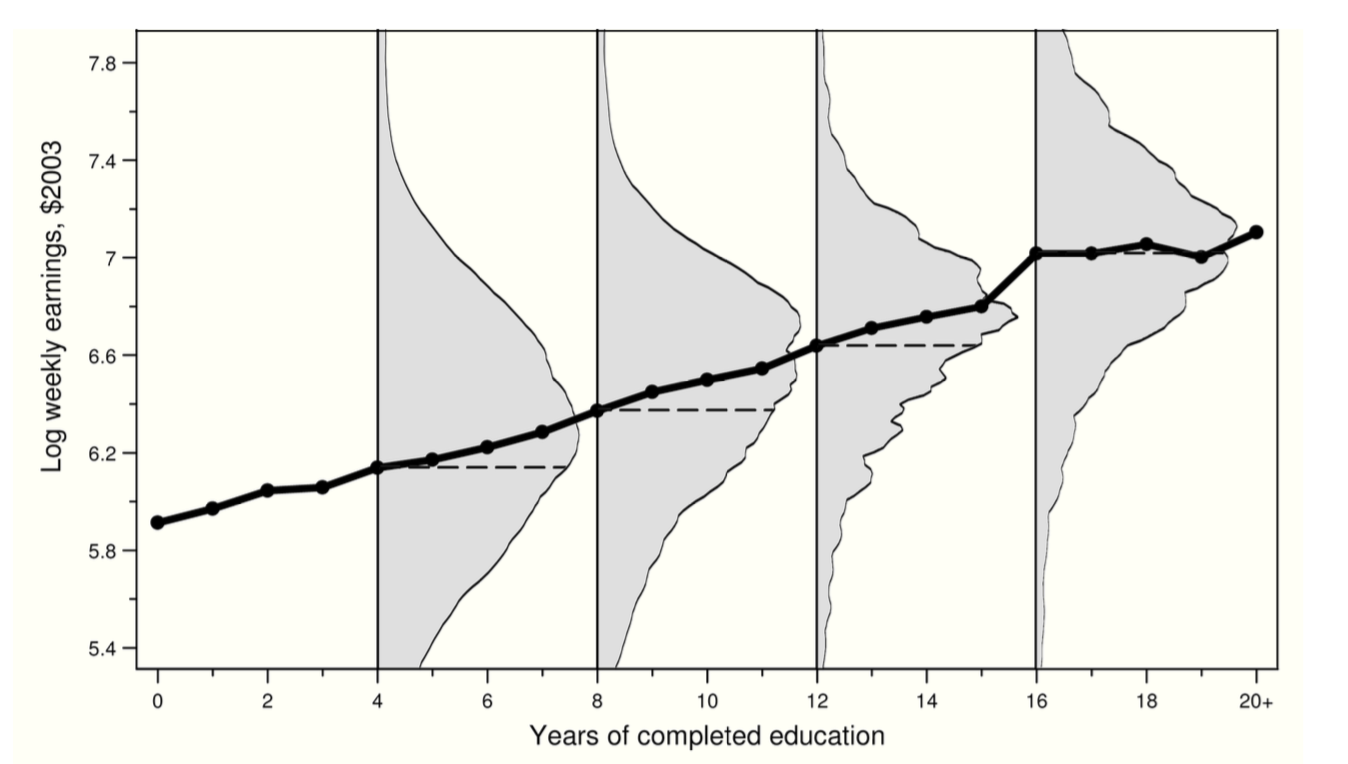
\includegraphics{figures/EarningsEducation}}
\end{figure}

}

\frame{

Discrete:
$$
\E[Y | x] =  \sum_{y \in \Supp(Y)} y f_{Y|X}(y | x)
$$

Continuous:

$$
\E[Y | x] =  \int_{-\infty}^{\infty} y f_{Y|X}(y | x) dy
$$

}

\frame{
Everything else carries through, just as though you were operating on a univariate PMF/PDF

\vspace{0.2in}

E.g., $$V[Y | x] = E[Y^2 | x] - E[Y | x]^2.$$
}

\frame{
Some other rules. Moving from conditional expectations to unconditional expectations.

\vspace{0.2in}

The {\it law of iterated expectations}:
$$
\E[Y] = \E_X \left[ \E[Y | X] \right],
$$
where $\E_X$ refers to the expectation over $X$.

\vspace{0.2in}

Draw on board.

%[I will sometimes be lazy in using just $\E_X$ or just $\E$. Both are correct, $\E_X$ just makes it clearer.]
}


%\frame{
%
%Proof sketch (with example on board), discrete:
%
%
%\begin{align*}
%\E[Z] & =  \sum_{x \in \Supp(X)} \sum_{y \in \Supp(Y)} h(x,y) f(x,y) \\
%& =  \sum_{x \in \Supp(X)} \sum_{y \in \Supp(Y)} h(x,y) f_X(x) f_{Y|X} (y |x) \\
%& =  \sum_{x \in \Supp(X)}  \left[ \sum_{y \in \Supp(Y)} h(x,y)  f_{Y|X} (y |x) \right] f_X(x) \\
%& =  \sum_{x \in \Supp(X)}  \E[Z | x] f_X(x) \\
%& =  \E_X \left[  \E[Z | x] \right].
%\end{align*}
%
%}

%\frame{
%
%Illustration. Suppose we had a random variable that had
%$$
%f(x,y) = \left\{
%     \begin{array}{lr}
%       1/3 & : x = 0, y = 0\\
%        1/3 & : x = 0, y = 1\\
%        1/3 & : x = 1, y = 0
%     \end{array}
%   \right.
%$$
%
%And $Z = h(X,Y) = x + y$. Then $\E[Z] = 2/3$.
%
%}
%
%\frame{
%
%
%
%}


%%%%% Proof sketch for law of iterated expectations. Another way to think about it? Sum of sum.

\frame{
Law of iterated expectations directly yields {\it law of total variance}:
$$
V[Y] = \E_X \left[ V[Y | X] \right] + V_X \left[ \E[Y | X] \right].
$$

Practically speaking, we can decompose the variability of a R.V. $Y$ into the average variability ``within" covariate values of $X$ and the average variability ``across" covariate values of $X$.

%Do proof. Example on board.

}



\frame{

\begin{center}
The conditional expectation function and the best [linear] predictor thereof.
\end{center}

}

\frame{

For the random vector $(X,Y)$, the conditional expectation function (CEF) is a function that takes as an input $x$ and returns the conditional expectation of $Y$ given $x$.

\vspace{0.2in}


Discrete:
$$
\E[Y | x] =  \sum_{y \in \Supp(Y)} y f_{Y|X}(y | x)
$$

Continuous:

$$
\E[Y | x] =  \int_{-\infty}^{\infty} y  f_{Y|X}(y | x) dy
$$
}

%\frame{
%
%Example. CEF of $X$ given $y$.
%
%\vspace{0.2in}
%
%
%$$
%f_{Y|X}(y | x = 1) = \left\{
%     \begin{array}{lr}
%       1/3 & : y \in \{1,2,3\}\\
%		 0 & : otherwise
%     \end{array}
%   \right.
%$$
%
%$$
%f_{Y|X}(y | x = 0) = \left\{
%     \begin{array}{lr}
%       2/9 & : y \in \{4,5,6\} \\
%       1/9 & : y \in \{1,2,3\} \\
%		 0 & : otherwise
%     \end{array}
%   \right.
%$$
%}
%
%\frame{
%
%Example. CEF of $Y$ given $x$.
%
%\vspace{0.2in}
%
%$$\E[Y | x = 1] = 2$$
%
%$$
%f_{Y|X}(Y | x = 0) = \left\{
%     \begin{array}{lr}
%       2/9 & : y \in \{4,5,6\} \\
%       1/9 & : y \in \{1,2,3\} \\
%		 0 & : otherwise
%     \end{array}
%   \right.
%$$
%}
%
%\frame{
%
%Example. CEF of $X$ given $y$.
%
%\vspace{0.2in}
%
%$$\E[Y | x = 1] = 2$$
%
%$$\E[Y | x = 0] = 4$$
%
%}

%\frame{
%
%Properties of deviations from the CEF.
%
%\vspace{0.2in}
%
%Define the R.V. $\epsilon = Y - \E[Y|X]$.
%
%\vspace{0.2in}
%
%\begin{itemize}
%\item $\E[\epsilon] = 0$
%\item $C(h(X), \epsilon) = 0$
%\item $V[\epsilon] = \E\left[V[Y | X]\right]$.
%\end{itemize}
%
%}

\frame{

\begin{center}
The CEF is the best (MMSE) predictor of $Y$ given $X=x$.
\end{center}

}

% This is where the class ended. Need more explanation of law of iterated expectations.

\frame{

I.e., suppose you knew the full joint CDF of $Y$ and $X$. And then someone gave you a randomly drawn value of $X$. What would be our guess of $Y$ that would have the lowest MSE?

\vspace{0.2in}

The answer is given by the CEF. The function $g(X)$ that best approximates $Y$ is the CEF.

}

%\frame{
%Proof sketch. Choose any function $g(X)$ to approximate $Y$.
%
%\vspace{0.2in}
%
%Define $U = Y - g(X)$.
%
% By the definition of MMSE, our goal is to choose $g(X)$ to minimize $\E[U^2]$.
%
% \vspace{0.2in}
%
% Define:
%
% $\epsilon = Y - E[Y | X]$
%
% $W = E[Y | X] - g(X)$
%
%  \vspace{0.2in}
%
% So that: $U = \epsilon  + W$.
%
%}
%
%\frame{
%
%Our goal is to show that, by choosing $g(X) = E[Y | X]$, we will minimize $\E[U^2]$.
%
%  \vspace{0.2in}
%
%
% $$\E[U^2 | x] = \E[ (\epsilon + w)^2] = \E[ \epsilon^2] + 2 w \E[\epsilon]+ w^2 = V[Y | x] + w^2,$$
%where $w = E[Y | x] - g(x)$.
%
%  \vspace{0.2in}
%
%
%Applying law of iterated expectations:
%
%$$
%\E[U^2] = \E \left[  V[Y | X] + w^2 \right] = \E \left[  V[Y | X] \right] + \E \left[ W^2\right].
%$$
%
%$\E \left[  V[Y | X] \right]$ does not depend on the choice of $g(x)$. And $ \E \left[ W^2\right] \geq 0$ with equality holding if $g(x) = \E[Y | x]$. Therefore, choosing $g(X) =  \E[Y | X]$ minimizes MSE.
%
%}

\frame{

But what if we were to restrict ourselves {\it only} to linear functions? I.e., let $g(X) = a + b X$.

  \vspace{0.2in}

By choosing the $a$ and $b$ that minimize MSE, we are using the best {\it linear} predictor (BLP) of $Y$ given $X$.

}

%\frame{
%Proof sketch. Apply the first order condition, minimizing $\E[U^2]$, where $U = Y - (a + bX)$.
%
%  \vspace{0.2in}
%
%By linearity of expectations + chain rule,
%$$
%\frac{\partial \E[U^2]}{\partial a} = \E\left[ \frac{\partial U^2}{\partial a}  \right] =  \E\left[ 2 U \frac{\partial U}{\partial a}  \right] = -2 \E[U] = 0 $$
%
%$$
%\frac{\partial \E[U^2]}{\partial b} = \E\left[ \frac{\partial U^2}{\partial b}  \right] = \E\left[ 2 U \frac{\partial U}{\partial b}  \right] = -2 \E[U X] = 0
%$$
%
%Then just solve: $\E[Y - (a + bX)] = 0$ and $\E[(Y - (a + bX) ) X] = 0$.
%
%  \vspace{0.2in}
%
%Rearranging equations: $b = C[X,Y]/V[X]$, $a = \E[Y] - b \E[X]$.
%
%}

\frame{

The BLP, among all functions $g(X) = a + bX$ is given by the constant
$$
a = \E[Y] -  C[X,Y]/V[X] \E[X]
$$
and the slope
$$
b = C[X,Y]/V[X].
$$

\bigskip

The proof is very similar to what we did for LS regression solution.

}


\frame{

Important corollaries:

\begin{itemize}
\item The BLP is also the best linear approximation to the CEF. (I.e., the optimal $a$ and $b$ minimizes $\E\left[  \left[ \E[Y | X] - (a + bX) \right]^2 \right]$. %The proof is obtained by the same means as above.
\item If the CEF {\it is} linear, the CEF is the BLP.
\end{itemize}

}

\frame{
\frametitle{BLP vs CEF}

\begin{figure}[ht] \centering
        \scalebox{.4}{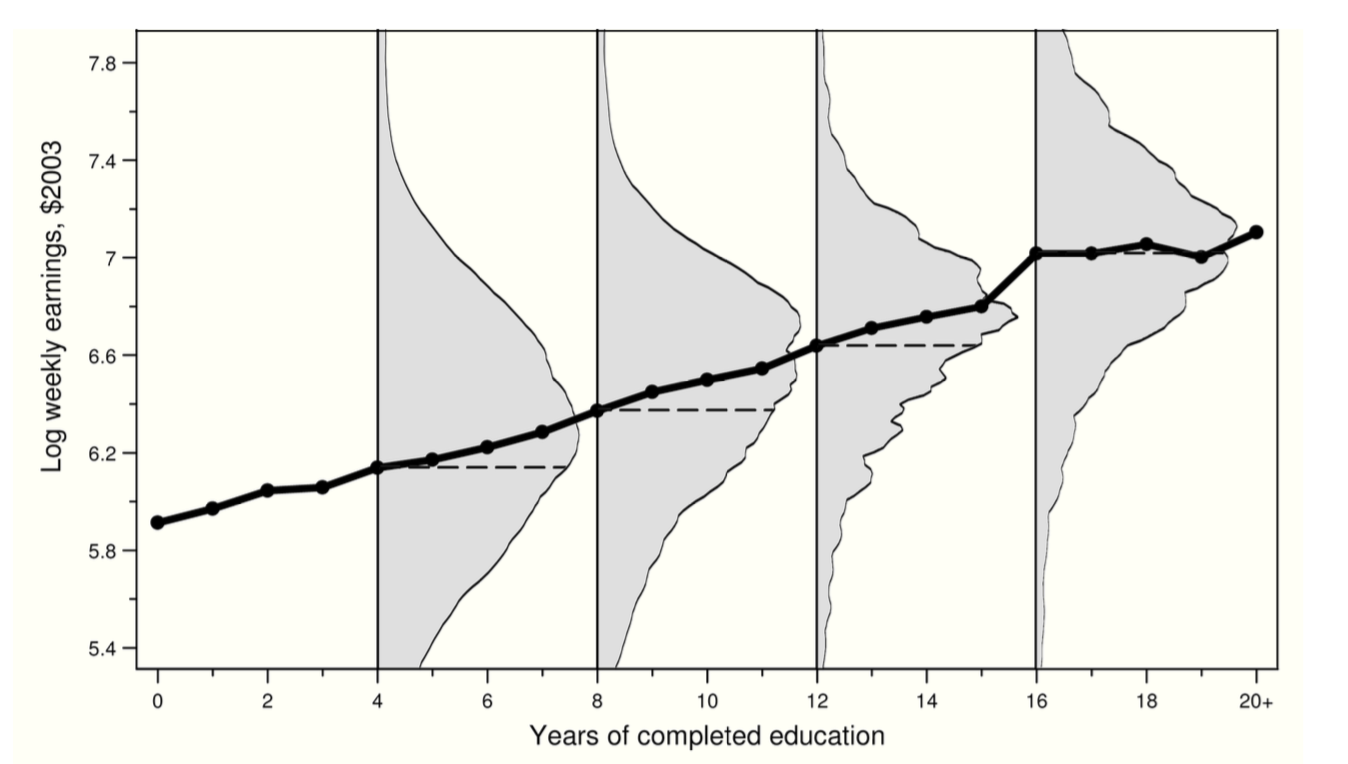
\includegraphics{figures/EarningsEducation}}
\end{figure}


}






% Might want to do it earlier

%\frame{
%
%Random sampling from some R.V. Real data!
%
%}
%
%\frame{
%
%Thus far, we have discussed what the properties of a R.V. (a theoretical construct) are.
%}
%
%\frame{
%
%What can we learn about the R.V. if we were to have repeated, random draws from the R.V.?
%
%}
%
%\frame{
%
%Under suitable regularity conditions, with infinite draws from an R.V., we can learn {\it everything} about its CDF
%
%}
%
%\frame{
%
%With a finite $n$ (number of draws from the R.V.), we can produce {\it estimates} of everything about its CDF [A formal definition of an estimate will have to wait!]
%
%}
%
%\frame{
%For now, we're going to focus on the properties of one {\it sample statistic}: the sample mean.
%}
%

\frame{
Sept. 27: What can we learn from a random sample?

}

\frame{
\frametitle{Why study random samples?}

\begin{itemize}
\item Often good design to learn about population averages. E.g., confirmed COVID-19 rates are typically undercounts, and a relatively small randomized sample testing regime may provide better estimates. \pause
\item Often good design to learn about population interventions. E.g, random assignment of bed nets to households may tell us something about the outcomes of a more widespread provision of bed nets on mosquito borne illness.\pause
\item Often a good provisional model for the first stage of research. E.g., those going to COVID testing centers may approximate a random sample from some subset of the population. Second stage of the research might be to learn about that subset compared to the overall population. \pause
\item Transformations used in forecasting can also be conceptualized in terms of random sampling. 
\end{itemize}

}

\frame{
\frametitle{Why study i.i.d. samples?}

\begin{itemize}
\item Equivalent to a random sample with replacement. \pause
\item Very good approximation for a random sample without replacement.
\end{itemize}

}



%\frame{
%\frametitle{Understanding i.i.d.}
%Ultra-mini math camp! Necessary for what we're going to do next.
%
%\begin{itemize}
%\item Chebyshev's inequality
%%\item Jensen's inequality
%\item Properties of independent random variables
%\end{itemize}
%}
%
%\frame{
%Chebyshev's inequality. (Bounds how much of the probability mass can be more than a few standard deviations away from the expected value, even if we don't know anything else about the R.V.)
%
%\vspace{0.2in}
%
%Given R.V. $X$ with finite $\E[X]$ and finite $V(X) > 0$. Then for any $k > 0$,
%$$
%\Pr\left( \left |X - \E[X] \right| \geq k \sqrt{V(X)} \right) \leq \frac{1}{k^2}
%$$
%or, equivalently,
%$$
%\Pr\left( | X - \E[X] | \geq k \right) \leq \frac{V(X)}{k^2}.
%$$
%
%Simple proof in Goldberger (1991), p. 31, via Markov's inequality.
%
%}
%
%\frame{
%
%Jensen's inequality.
%
%$\E[f(X)] \leq f(\E[X])$ for concave $f(.)$.
%
%\vspace{0.2in}
%
%
%Corollary:
%
%$\E[f(X)] \geq f(\E[X])$ for convex $f(.)$.
%
%
%}
%
%
%\frame{
%\begin{center}
%\includegraphics[width=1\textwidth]{jensen.PDF}
%\end{center}
%Image blatantly cribbed from \url{http://mathstat.helsinki.fi/~kisdi/mathmet/lecturenotes.PDF}
%}

\frame{
\frametitle{Understanding i.i.d.}

What does i.i.d. stand for:
\begin{itemize}
\item Independent (i.e., observations independent from each other)
\item Identically distributed (i.e., all observations drawn from same distribution)
\end{itemize}

}

\frame{
\frametitle{Implications of independence}



$Y_1$ and $Y_2$ are {\it independent} if and only if $f_{Y_1,Y_2}(y_1,y_2) = f_{Y_1}(y_1) \cdot f_{Y_2}(y_2),$ for all $(y_1,y_2)$.

\bigskip

If $Y_1$ and $Y_2$ are independent, then:
\vspace{0.2in}

\begin{itemize}
\item Covariance is zero: $$C(Y_1,Y_2) = 0.$$
\item Variances are additive: $$
V(Y_1 +Y_2) = V(Y_1) + V(Y_2).
$$
%\item If $Z_X = f(X)$ and $Z_Y = g(Y)$, then $Z_X$ and $Z_Y$ are independent.
\end{itemize}

}

\frame{
\frametitle{Implications of identically distributed}

$Y_1$ and $Y_2$ are {\it independent} if and only if $f_{Y_1,Y_2}(y_1,y_2) = f_{Y_1}(y_1) \cdot f_{Y_2}(y_2),$ for all $(y_1,y_2)$.

\bigskip

$Y_1$ and $Y_2$ are {\it identically distributed} if and only if  $f_{Y_1}(y_1) = f_{Y_2}(y_2)$ for all $(y_1,y_2)$.


}

%\frame{
%
%Suppose we have an {\it independent and identically distributed} (i.i.d) random sample of $n$ observations all drawn from some R.V. $Y$.
%
%\vspace{0.2in}
%
%I.e., we draw from the R.V. $Y$. Then we draw from $Y$ again, in such a manner that our 2nd draw does not depend on the first draw. And then repeat this process until we have $n$ draws.
%
%
%
%}


%\frame{
%
%Note that if we take a random sample from a large population, and we randomly assign half of the units to treatment and half to control, we will approximately have two i.i.d. samples.
%
%\begin{align*}
%(Y_1(1),Y_2(1),...,Y_{n/2}(1)) &\sim_{i.i.d.} F_{Y(1)} \\
%(Y_{n/2+1}(0),Y_{n/2+2}(0),...,Y_{n}(0)) &\sim_{i.i.d.} F_{Y(0)}
%\end{align*}
%
%\vspace{0.2in}
%
%For the rest of this, when you see $Y$, you can also think $Y(1)$.
%}

\frame{
So, we have $n$ random variables that generate $n$ values.

\vspace{0.2in}

We can subscript each of these $n$ random variables, as well as aggregate them.

\vspace{0.2in}


The random vector $\mathbf{Y} = (Y_1,...,Y_n)'$.

}

\frame{

Under the assumption of {\it random sampling} from $F_Y$, the collection of values that you see are each produced by an identical random process.

\vspace{0.2in}

The actual values that we observe are denoted with $\mathbf{y} = (y_1,...,y_n)'$.

\vspace{0.2in}

For now, we focus on learning about the population mean ($\E[Y]=\mu$), although to do so, we will need to also learn about the nuisance parameter ($V[Y]$).

\vspace{0.2in}

We want an estimator with small mean squared error (recall that this is equivalent to squared bias plus variance) and an estimator that allows the production of tight confidence intervals.
}

\frame{
A sample statistic {\it summarizes} those $n$ values. When used to estimate a population parameter, also considered an estimator.

\bigskip
Sample mean:
$$
\widehat \mu_{sample~mean} = \overline Y = \frac{\sum_{i=1}^n Y_i}{n} = \frac{1}{n} \left( Y_1 + ... +Y_n \right) .
$$

\bigskip

Class of linear combinations:
$$
\widehat \mu_{\mathbf{c}} = \sum_{i=1}^n c_i Y_i = \left(c_1 Y_1 + ...+ c_n Y_n \right) .
$$

}

\frame{
Which column is the sampling distribution of the sample mean
\begin{table}[h]
\begin{center}
{\scriptsize
\begin{tabular}{r|r|r|r|r|r} %cc
$i$ & \multicolumn{1}{r|}{1} & \multicolumn{1}{r|}{2}   & $\dots$ & \multicolumn{1}{r|}{625} & \\ % & \multicolumn{1}{c}{$MoE$}& \multicolumn{1}{c}{95\% CI}  \\
$s$  & $Y_1$  & $Y_2$   & $\dots$  & $Y_{625}$  & $\overline{Y}_{625}$ \\ % & $2\cdot\sqrt{\frac{\overline{Y}_{625}(1-\overline{Y}_{625})}{625}}$ & $\overline{Y}_{625} \pm MoE$ \\
\hline
1 & 35 & 50   & $\dots$  & 22 & 45  \\ %& \visible<2->{.037} & \visible<3->{[.643,.717]}\\
2 & 28 & 19   & $\dots$  & 65 & 47 \\ %& \visible<2->{.037}  & \visible<3->{[.663,.737]}\\
3 & 33 & 27  & $\dots$  & 45 & 42 \\ %& \visible<2->{.035} & \visible<3->{[.715,.785]}\\
4 & $\vdots$ & $\vdots$ & $\dots$  & $\vdots$ & $\vdots$ \\ %& \visible<2->{.036} & \visible<3->{[.694,.766]}\\
5 & $\vdots$ & $\vdots$  & $\dots$  & $\vdots$ & $\vdots$ \\ %& \visible<2->{.037} & \visible<3->{[.653,.727]}\\
$\vdots$ & $\vdots$  & $\vdots$ & $\vdots$ & $\vdots$  & $\vdots$ \\ % & \visible<2->{$\vdots$} & \visible<3->{$\vdots$}  \\
1 mil  & 41 & 53& $\dots$  & 21 & 46 \\ %& \visible<2->{.035}& \visible<3->{[.705,.775]}\\
 $\vdots$  & $\vdots$  & $\vdots$ & $\vdots$ & $\vdots$  & $\vdots$ \\ % & \visible<2->{$\vdots$} & \visible<3->{$\vdots$}\\
\hline
\visible<1->{$f_{\cdot}(\cdot)$} & \multicolumn{1}{r|}{\visible<1->{?}} & \multicolumn{1}{r|}{\visible<1->{?}}  & & \multicolumn{1}{r|}{\visible<1->{?}} & \visible<1->{?} \\
\visible<1->{$\E_{\cdot}(\cdot)$} & \multicolumn{1}{r|}{\visible<1->{45}} & \multicolumn{1}{r|}{\visible<1->{45}}  & & \multicolumn{1}{r|}{\visible<1->{45}} & \visible<1->{?} \\
\visible<1->{$V_{\cdot}(\cdot)$} & \multicolumn{1}{r|}{\visible<1->{25}} & \multicolumn{1}{r|}{\visible<1->{25}}  & & \multicolumn{1}{r|}{\visible<1->{25}} & \visible<1->{?} \\
\end{tabular}}
%\caption{\emph{Sampling Distributions for $\overline{Y}_{625}$, the Margin-of-Error, and the 95\% Confidence Interval}}\label{t:samdistCI}
\end{center}
\end{table}

}




\frame{
Property \#1: {\it The sample mean is unbiased for the population mean.} The expected value of the sample mean,
$\E[\overline Y] = \E[Y]$.

\vspace{0.2in}

Proof:
\begin{align*}
\E[\overline Y] &= \E \left[ \frac{1}{n} \left( Y_1 + ... + Y_n \right) \right] \\
& =  \\%\frac{1}{n} \E \left[ Y_1 + ... + Y_n  \right] \\
& =  \\%\frac{1}{n} \left( \E [ Y_1] + ... + \E [Y_n]  \right) \\
& =  \\%\frac{1}{n} \left( \E [ Y] + ... + \E [Y]  \right) \\
& =  \\%\frac{1}{n} n \E [ Y] \\
& = \E[Y_1].
\end{align*}

}

\frame{
The sample mean is unbiased
\begin{table}[h]
\begin{center}
{\scriptsize
\begin{tabular}{r|r|r|r|r|r} %cc
$i$ & \multicolumn{1}{r|}{1} & \multicolumn{1}{r|}{2}   & $\dots$ & \multicolumn{1}{r|}{625} & \\ % & \multicolumn{1}{c}{$MoE$}& \multicolumn{1}{c}{95\% CI}  \\
$s$  & $Y_1$  & $Y_2$   & $\dots$  & $Y_{625}$  & $\overline{Y}_{625}$ \\ % & $2\cdot\sqrt{\frac{\overline{Y}_{625}(1-\overline{Y}_{625})}{625}}$ & $\overline{Y}_{625} \pm MoE$ \\
\hline
1 & 35 & 50   & $\dots$  & 22 & 45  \\ %& \visible<2->{.037} & \visible<3->{[.643,.717]}\\
2 & 28 & 19   & $\dots$  & 65 & 47 \\ %& \visible<2->{.037}  & \visible<3->{[.663,.737]}\\
3 & 33 & 27  & $\dots$  & 45 & 42 \\ %& \visible<2->{.035} & \visible<3->{[.715,.785]}\\
4 & $\vdots$ & $\vdots$ & $\dots$  & $\vdots$ & $\vdots$ \\ %& \visible<2->{.036} & \visible<3->{[.694,.766]}\\
5 & $\vdots$ & $\vdots$  & $\dots$  & $\vdots$ & $\vdots$ \\ %& \visible<2->{.037} & \visible<3->{[.653,.727]}\\
$\vdots$ & $\vdots$  & $\vdots$ & $\vdots$ & $\vdots$  & $\vdots$ \\ % & \visible<2->{$\vdots$} & \visible<3->{$\vdots$}  \\
1 mil  & 41 & 53& $\dots$  & 21 & 46 \\ %& \visible<2->{.035}& \visible<3->{[.705,.775]}\\
 $\vdots$  & $\vdots$  & $\vdots$ & $\vdots$ & $\vdots$  & $\vdots$ \\ % & \visible<2->{$\vdots$} & \visible<3->{$\vdots$}\\
\hline
\visible<1->{$f_{\cdot}(\cdot)$} & \multicolumn{1}{r|}{\visible<1->{?}} & \multicolumn{1}{r|}{\visible<1->{?}}  & & \multicolumn{1}{r|}{\visible<1->{?}} & \visible<1->{?} \\
\visible<1->{$\E_{\cdot}(\cdot)$} & \multicolumn{1}{r|}{\visible<1->{45}} & \multicolumn{1}{r|}{\visible<1->{45}}  & & \multicolumn{1}{r|}{\visible<1->{45}} & \visible<1->{\textcolor{red}{45}} \\
\visible<1->{$V_{\cdot}(\cdot)$} & \multicolumn{1}{r|}{\visible<1->{25}} & \multicolumn{1}{r|}{\visible<1->{25}}  & & \multicolumn{1}{r|}{\visible<1->{25}} & \visible<1->{?} \\
\end{tabular}}
%\caption{\emph{Sampling Distributions for $\overline{Y}_{625}$, the Margin-of-Error, and the 95\% Confidence Interval}}\label{t:samdistCI}
\end{center}
\end{table}

}


\frame{

Within the class of linear combinations, what must be true for unbiasedness?

$$
\widehat \mu_{\mathbf{c}} = \sum_{i=1}^n c_i Y_i = \left(c_1 Y_1 + ...+ c_n Y_n \right) .
$$

}




\frame{
Property \#2: The {\it sampling variance} of the sample mean,
$$V[\overline Y] = \frac{V[Y]}n.$$

\vspace{0.2in}

Proof:
\begin{align*}
V[\overline Y] &= V \left[ \left(  \frac{1}{n} Y_1 + ...  + \frac{1}{n} Y_n \right) \right] \\
&= \\%\frac{1}{n^2}  V \left[ Y_1 + ...  + Y_n \right] \\
& =  \\% \frac{1}{n^2}   \left( V[Y_1] + ...  + V[Y_n] \right) \\
& =  \\%\frac{1}{n^2}   \left( V[Y] + ...  + V[Y] \right) \\
& =  \\%\frac{1}{n^2}   n V[Y] \\
& =  \frac{1}{n}   V[Y].
\end{align*}

}

\frame{
Sampling distribution of the sample mean
\begin{table}[h]
\begin{center}
{\scriptsize
\begin{tabular}{r|r|r|r|r|r} %cc
$i$ & \multicolumn{1}{r|}{1} & \multicolumn{1}{r|}{2}   & $\dots$ & \multicolumn{1}{r|}{625} & \\ % & \multicolumn{1}{c}{$MoE$}& \multicolumn{1}{c}{95\% CI}  \\
$s$  & $Y_1$  & $Y_2$   & $\dots$  & $Y_{625}$  & $\overline{Y}_{625}$ \\ % & $2\cdot\sqrt{\frac{\overline{Y}_{625}(1-\overline{Y}_{625})}{625}}$ & $\overline{Y}_{625} \pm MoE$ \\
\hline
1 & 35 & 50   & $\dots$  & 22 & 45  \\ %& \visible<2->{.037} & \visible<3->{[.643,.717]}\\
2 & 28 & 19   & $\dots$  & 65 & 47 \\ %& \visible<2->{.037}  & \visible<3->{[.663,.737]}\\
3 & 33 & 27  & $\dots$  & 45 & 42 \\ %& \visible<2->{.035} & \visible<3->{[.715,.785]}\\
4 & $\vdots$ & $\vdots$ & $\dots$  & $\vdots$ & $\vdots$ \\ %& \visible<2->{.036} & \visible<3->{[.694,.766]}\\
5 & $\vdots$ & $\vdots$  & $\dots$  & $\vdots$ & $\vdots$ \\ %& \visible<2->{.037} & \visible<3->{[.653,.727]}\\
$\vdots$ & $\vdots$  & $\vdots$ & $\vdots$ & $\vdots$  & $\vdots$ \\ % & \visible<2->{$\vdots$} & \visible<3->{$\vdots$}  \\
1 mil  & 41 & 53& $\dots$  & 21 & 46 \\ %& \visible<2->{.035}& \visible<3->{[.705,.775]}\\
 $\vdots$  & $\vdots$  & $\vdots$ & $\vdots$ & $\vdots$  & $\vdots$ \\ % & \visible<2->{$\vdots$} & \visible<3->{$\vdots$}\\
\hline
\visible<1->{$f_{\cdot}(\cdot)$} & \multicolumn{1}{r|}{\visible<1->{?}} & \multicolumn{1}{r|}{\visible<1->{?}}  & & \multicolumn{1}{r|}{\visible<1->{?}} & \visible<1->{?} \\
\visible<1->{$\E_{\cdot}(\cdot)$} & \multicolumn{1}{r|}{\visible<1->{45}} & \multicolumn{1}{r|}{\visible<1->{45}}  & & \multicolumn{1}{r|}{\visible<1->{45}} & \visible<1->{\textcolor{black}{45}} \\
\visible<1->{$V_{\cdot}(\cdot)$} & \multicolumn{1}{r|}{\visible<1->{25}} & \multicolumn{1}{r|}{\visible<1->{25}}  & & \multicolumn{1}{r|}{\visible<1->{25}} & \visible<1->{\textcolor{red}{$\frac{25}{625}$}} \\
\end{tabular}}
%\caption{\emph{Sampling Distributions for $\overline{Y}_{625}$, the Margin-of-Error, and the 95\% Confidence Interval}}\label{t:samdistCI}
\end{center}
\end{table}

}

\frame{

Within the class of linear combinations, what is the variance in terms of $\mathbf{c}$?

$$
\widehat \mu_{\mathbf{c}} = \sum_{i=1}^n c_i Y_i = \left(c_1 Y_1 + ...+ c_n Y_n \right) .
$$

What does this expression tell us about minimizing variance?

}

%
%%\frame{
%%The WLLN is a deeply profound result, and it's one that we've hinted at all along. In fact, let's try something a little clever.
%%}
%
%
%\frame{
%
%So random samples tell us a lot about means, but suppose we wanted to estimate the entire distribution. \\
%
%\bigskip
%
%Remember the CDF is defined in terms of
%$$
%\Pr(Y \leq c).
%$$
%for all values of $c$.
%
%%[Remember: I have not formally defined an estimator yet.]
%}
%
%\frame{
%Define a random variable $Z = \I[ Y \leq c]$, where $\I[.]$ is the indicator function (takes the value 1 if true, 0 if false). Then
%
%$$
%\E[Z] = \Pr(Y \leq c).
%$$
%
%Proof. $$\Pr(Z = 1) = \Pr(Y \leq c),$$ Then, by the definition of the expected value, $$\E[Z] = \Pr(Y \leq c) \times 1 + \Pr(Y > c) \times 0 = \Pr(Y \leq c).$$
%
%
%\bigskip
%
%Hence, learning about means can tell us about the whole distribution.
%
%}
%
%\frame{
%By property \#4 then,
%
%$$
%\overline Z \arrowp  \Pr(Y \leq c).
%$$
%
%}
%
%\frame{
%We could do this for any or every value of $c$. Which is to say, we can always approximate the CDF to arbitrary precision. If $n$ is very large, the probability that we're wrong for a given point of the CDF by much is very small.
%
%\vspace{0.2in}
%
%Stronger results are possible under weaker assumptions. Strong LLN and Glivenko-Cantelli. %We will discuss these later.
%
%}
%
%
%\frame{
%
%This is why so-called identification results work directly off the probability distribution of $Y$. Even if we don't {\it know} $Y$, we can learn everything about $Y$ (with diminishing uncertainty) just by drawing repeated values from $Y$.
%
%}
%
%
%\frame{
%Sampling distribution of the sample mean
%\begin{table}[h]
%\begin{center}
%{\scriptsize
%\begin{tabular}{r|r|r|r|r|r|r} %cc
%$i$ & \multicolumn{1}{r|}{1} & \multicolumn{1}{r|}{2}   & $\dots$ & \multicolumn{1}{r|}{625} & & \\ % & \multicolumn{1}{c}{$MoE$}& \multicolumn{1}{c}{95\% CI}  \\
%$s$  & $Y_1$, $Z_{1}^{40}$ & $Y_2$, $Z_{2}^{40}$   & $\dots$  & $Y_{625}$,$Z_{625}^{40}$  & $\overline{Y}_{625}$ & $\overline{Z}_{625}^{40}$\\ % & $2\cdot\sqrt{\frac{\overline{Y}_{625}(1-\overline{Y}_{625})}{625}}$ & $\overline{Y}_{625} \pm MoE$ \\
%\hline
%1 & 35,1 & 50,0   & $\dots$  & 22,1 & 45 &.45 \\ %& \visible<2->{.037} & \visible<3->{[.643,.717]}\\
%2 & 28,1 & 19,1   & $\dots$  & 65,0 & 47 &.38\\ %& \visible<2->{.037}  & \visible<3->{[.663,.737]}\\
%3 & 33,1 & 27,1  & $\dots$  & 45,0 & 42 &.56\\ %& \visible<2->{.035} & \visible<3->{[.715,.785]}\\
%4 & $\vdots$ & $\vdots$ & $\dots$  & $\vdots$ & $\vdots$ \\ %& \visible<2->{.036} & \visible<3->{[.694,.766]}\\
%5 & $\vdots$ & $\vdots$  & $\dots$  & $\vdots$ & $\vdots$ \\ %& \visible<2->{.037} & \visible<3->{[.653,.727]}\\
%$\vdots$ & $\vdots$  & $\vdots$ & $\vdots$ & $\vdots$  & $\vdots$ \\ % & \visible<2->{$\vdots$} & \visible<3->{$\vdots$}  \\
%1 mil  & 41,0 & 53,0& $\dots$  & 21,1 & 46 &.41\\ %& \visible<2->{.035}& \visible<3->{[.705,.775]}\\
% $\vdots$  & $\vdots$  & $\vdots$ & $\vdots$ & $\vdots$  & $\vdots$ \\ % & \visible<2->{$\vdots$} & \visible<3->{$\vdots$}\\
%\hline
%\visible<1->{$f_{\cdot}(\cdot)$} & \multicolumn{1}{r|}{\visible<1->{?}} & \multicolumn{1}{r|}{\visible<1->{?}}  & & \multicolumn{1}{r|}{\visible<1->{?}} & \visible<1->{?} \\
%\visible<1->{$\E_{\cdot}(\cdot)$} & \multicolumn{1}{r|}{\visible<1->{45}} & \multicolumn{1}{r|}{\visible<1->{45}}  & & \multicolumn{1}{r|}{\visible<1->{45}} & \visible<1->{\textcolor{black}{45}} & $\E[Z^{40}]$ \\
%\visible<1->{$V_{\cdot}(\cdot)$} & \multicolumn{1}{r|}{\visible<1->{25}} & \multicolumn{1}{r|}{\visible<1->{25}}  & & \multicolumn{1}{r|}{\visible<1->{25}} & \visible<1->{\textcolor{black}{$\frac{25}{625}$}} \\
%\end{tabular}}
%%\caption{\emph{Sampling Distributions for $\overline{Y}_{625}$, the Margin-of-Error, and the 95\% Confidence Interval}}\label{t:samdistCI}
%\end{center}
%\end{table}
%
%}
%
%\frame{
%Sampling distribution of the sample mean
%\begin{table}[h]
%\begin{center}
%{\scriptsize
%\begin{tabular}{r|r|r|r|r|r|r|r} %cc
%$i$ & \multicolumn{1}{r|}{1} & \multicolumn{1}{r|}{2}   & $\dots$ & \multicolumn{1}{r|}{625} & && \\ % & \multicolumn{1}{c}{$MoE$}& \multicolumn{1}{c}{95\% CI}  \\
%$s$  & $Y_1$, $Z_{1}^{40}$, $Z_{1}^{41}$ & $Y_2$, $Z_{2}^{40}$, $Z_{2}^{41}$   & $\dots$  & $Y_{625}$,$Z_{625}^{40}$, $Z_{625}^{41}$  & $\overline{Y}_{625}$ & $\overline{Z}_{625}^{40}$ & $\overline{Z}_{625}^{41}$ \\ % & $2\cdot\sqrt{\frac{\overline{Y}_{625}(1-\overline{Y}_{625})}{625}}$ & $\overline{Y}_{625} \pm MoE$ \\
%\hline
%1 & 35,1,1 & 50,0,0   & $\dots$  & 22,1,1 & 45 &.45 &.46 \\ %& \visible<2->{.037} & \visible<3->{[.643,.717]}\\
%2 & 28,1,1 & 19,1,1   & $\dots$  & 65,0,0 & 47 &.38 & .38\\ %& \visible<2->{.037}  & \visible<3->{[.663,.737]}\\
%3 & 33,1,1 & 27,1,1  & $\dots$  & 45,0,0 & 42 &.56 & .56\\ %& \visible<2->{.035} & \visible<3->{[.715,.785]}\\
%4 & $\vdots$ & $\vdots$ & $\dots$  & $\vdots$ & $\vdots$   \\ %& \visible<2->{.036} & \visible<3->{[.694,.766]}\\
%5 & $\vdots$ & $\vdots$  & $\dots$  & $\vdots$ & $\vdots$   \\ %& \visible<2->{.037} & \visible<3->{[.653,.727]}\\
%$\vdots$ & $\vdots$  & $\vdots$ & $\vdots$ & $\vdots$  & $\vdots$   \\ % & \visible<2->{$\vdots$} & \visible<3->{$\vdots$}  \\
%1 mil  & 41,0,1 & 53,0,0& $\dots$  & 21,1,1 & 46 &.41 &.42  \\ %& \visible<2->{.035}& \visible<3->{[.705,.775]}\\
% $\vdots$  & $\vdots$  & $\vdots$ & $\vdots$ & $\vdots$  & $\vdots$  \\ % & \visible<2->{$\vdots$} & \visible<3->{$\vdots$}\\
%\hline
%\visible<1->{$f_{\cdot}(\cdot)$} & \multicolumn{1}{r|}{\visible<1->{?}} & \multicolumn{1}{r|}{\visible<1->{?}}  & & \multicolumn{1}{r|}{\visible<1->{?}} & \visible<1->{?} \\
%\visible<1->{$\E_{\cdot}(\cdot)$} & \multicolumn{1}{r|}{\visible<1->{45}} & \multicolumn{1}{r|}{\visible<1->{45}}  & & \multicolumn{1}{r|}{\visible<1->{45}} & \visible<1->{\textcolor{black}{45}} & $\E[Z^{40}]$ &$\E[Z^{41}]$ \\
%\visible<1->{$V_{\cdot}(\cdot)$} & \multicolumn{1}{r|}{\visible<1->{25}} & \multicolumn{1}{r|}{\visible<1->{25}}  & & \multicolumn{1}{r|}{\visible<1->{25}} & \visible<1->{\textcolor{black}{$\frac{25}{625}$}} \\
%\end{tabular}}
%%\caption{\emph{Sampling Distributions for $\overline{Y}_{625}$, the Margin-of-Error, and the 95\% Confidence Interval}}\label{t:samdistCI}
%\end{center}
%\end{table}
%
%}



%\frame{
%
%Jensen's inequality.
%
%$\E[f(Y)] \leq f(\E[Y])$ for concave $f(.)$.
%
%\vspace{0.2in}
%
%
%Corollary:
%
%$\E[f(Y)] \geq f(\E[Y])$ for convex $f(.)$.
%
%}


%\frame{
%\begin{center}
%\includegraphics[width=1\textwidth]{jensen.PDF}
%\end{center}
%Image blatantly cribbed from \url{http://mathstat.helsinki.fi/~kisdi/mathmet/lecturenotes.PDF}
%}



%\frame{
%
%So we can estimate the CDF with large samples, but we want to know how accurate we are for our sample with fixed size $n$.
%\begin{itemize}
%\item need to estimate variance
%\item use estimated variance for confidence intervals
%\end{itemize}
%
%
%}
%
%
%\frame{
%
%(A consequence of the) Continuous Mapping Theorem, stated loosely. Continuous functions are limit-preserving.
%
%\vspace{0.2in}
%
%For continuous $f(.)$, then if $Y \arrowp c$, then $f(Y) \arrowp f(c)$.
%
%\vspace{0.2in}
%
%%[If anyone has a clearer way to express this without adding any difficult math, I'm all ears!]
%
%}

\frame{
\frametitle{Learning about population variance}

\bi
\item We've shown that the sample mean is unbiased
\item We've shown that the variance of the sample mean is $V[Y]/n$
\item We still need to learn something about $V[Y]$
\ei

}

\frame{
Recall that the ``population" variance of a random variable $Y$:

$$
V(Y) = \E\left[ Y^2\right] -  \E[Y]^2
$$

}

\frame{

Can we propose an estimator of $V(Y)$?

}


\frame{
Put another way:

\begin{itemize}
\item Can we propose an estimator of $\E\left[ Y^2\right]$?
\item Can we propose an estimator of $ \E[Y]^2$?
\end{itemize}

}


\frame{

\begin{itemize}
\item Can we propose an estimator of $\E\left[ Y^2\right]$?
\begin{itemize}
\item Plug-in estimator: $$\overline{Y^2} = \frac{\sum_{i=1}^n Y^2_i}{n}.$$
\item $\E[\overline{Y^2}] = \E\left[ Y^2\right]$ (just let $Y^2=Z$ and it is just $\E[\overline{Z}] = \E\left[ Z\right]$).
%\item $\overline{Y^2} \arrowp \E\left[ Y^2\right]$.
\end{itemize}
\end{itemize}

}

%\frame{
%\begin{itemize}
%\item Can we propose an estimator of $ \E[Y]^2$?
%\begin{itemize}
%\item Plug-in estimator: $$\overline{Y}^2 = \left[\frac{\sum_{i=1}^n Y_i}{n}\right]^2.$$
%\item However, $\E[\overline{Y}^2] \neq \E\left[ Y\right]^2$ (Jensen's inequality).
%\item What does $\E[\overline{Y}^2]$ equal?
%\end{itemize}
%\end{itemize}
%}
%
%\frame{
%$$\E[\overline{Y}^2] = \E[Y]^2 + \frac{V[Y]}{n}$$
%Proof.
%\begin{align*}
%V[\overline{Y}] &= \E[\overline{Y}^2]  - \E[\overline{Y}]^2 \\
%V[\overline{Y}] &= \E[\overline{Y}^2]  - \E[Y]^2 \\
%V[\overline{Y}] + \E[Y]^2 &= \E[\overline{Y}^2]  \\
%\frac{V[Y]}{n} + \E[Y]^2 &= \E[\overline{Y}^2]
%\end{align*}
%}

\frame{
\begin{itemize}
\item Can we propose an estimator of $ \E[Y]^2$?
\begin{itemize}
\item Plug-in estimator: $$\overline{Y}^2 = \left[\frac{\sum_{i=1}^n Y_i}{n}\right]^2.$$
\item What is it's expectation ($\E[\overline{Y}^2] $)?
\item Recall that $V[\overline Y] = \E[\overline{Y}^2] - \E\left[ \overline Y\right]^2$
\item Simplifies to $\frac{V[Y]}{n} = \E[\overline{Y}^2] - \E\left[ Y\right]^2$
\item Rearranging shows that $\E[\overline{Y}^2] = \E\left[ Y\right]^2 + \frac{V[Y]}{n}$
%\item $\overline{Y}^2 \arrowp \E\left[ Y\right]^2$ (follows from CMT)
\end{itemize}
\end{itemize}
}

\frame{
Therefore, the plug-in estimator of variance,
$$
\overline{Y^2} - \overline{Y}^2.
$$
is biased:
\begin{align*}
\E[\overline{Y^2} - \overline{Y}^2] &= \E\left[ Y^2\right] - (\E\left[ Y\right]^2 + \frac{V[Y]}{n})\\
&= (\E\left[ Y^2\right] - \E\left[ Y\right]^) - \frac{V[Y]}{n})\\
&= V(Y) -  \frac{V[Y]}{n} \\
&= (1 - \frac{1}{n})V(Y) \\
&= \frac{n-1}{n}V(Y)
\end{align*}
}


\frame{
However, the bias can be corrected by multiplying the estimator by $\frac{n}{n-1}$:
$$
\hat V(Y) = \frac{n}{n-1} \left[ \overline{Y^2} - \overline{Y}^2\right].
$$
with
\begin{itemize}
\item $\E[\hat V(Y)] = \frac{n}{n-1}\E \left[ \overline{Y^2} - \overline{Y}^2\right]= \frac{n}{n-1} \frac{n-1}{n} V(Y)$
%\item $\hat V(Y) \arrowp V(Y)$.
\end{itemize}
This is what R computes when you type \texttt{var(.)}.
}

\frame{
Sampling distribution of the sample variance (fill in for biased sample variance)
\begin{table}[h]
\begin{center}
{\scriptsize
\begin{tabular}{r|r|r|r|r|rcc} %cc
$i$ & \multicolumn{1}{r|}{1} & \multicolumn{1}{r|}{2}   & $\dots$ & \multicolumn{1}{r|}{625} & \\ % & \multicolumn{1}{c}{$MoE$}& \multicolumn{1}{c}{95\% CI}  \\
$s$  & $Y_1$  & $Y_2$   & $\dots$  & $Y_{625}$  & $\overline{Y}_{625}$ & $\hat V(Y)$ & $\overline{Y^2} -  \overline{Y}^2$  \\ % & $2\cdot\sqrt{\frac{\overline{Y}_{625}(1-\overline{Y}_{625})}{625}}$ & $\overline{Y}_{625} \pm MoE$ \\
\hline
1 & 35 & 50   & $\dots$  & 22 & 45 & 20 \\ %& \visible<2->{.037} & \visible<3->{[.643,.717]}\\
2 & 28 & 19   & $\dots$  & 65 & 47  & 17\\ %& \visible<2->{.037}  & \visible<3->{[.663,.737]}\\
3 & 33 & 27  & $\dots$  & 45 & 42 & 38 \\ %& \visible<2->{.035} & \visible<3->{[.715,.785]}\\
4 & $\vdots$ & $\vdots$ & $\dots$  & $\vdots$ & $\vdots$ \\ %& \visible<2->{.036} & \visible<3->{[.694,.766]}\\
5 & $\vdots$ & $\vdots$  & $\dots$  & $\vdots$ & $\vdots$ \\ %& \visible<2->{.037} & \visible<3->{[.653,.727]}\\
$\vdots$ & $\vdots$  & $\vdots$ & $\vdots$ & $\vdots$  & $\vdots$ \\ % & \visible<2->{$\vdots$} & \visible<3->{$\vdots$}  \\
1 mil  & 41 & 53& $\dots$  & 21 & 46 & 32\\ %& \visible<2->{.035}& \visible<3->{[.705,.775]}\\
 $\vdots$  & $\vdots$  & $\vdots$ & $\vdots$ & $\vdots$  & $\vdots$ \\ % & \visible<2->{$\vdots$} & \visible<3->{$\vdots$}\\
\hline
\visible<1->{$f_{\cdot}(\cdot)$} & \multicolumn{1}{r|}{\visible<1->{?}} & \multicolumn{1}{r|}{\visible<1->{?}}  & & \multicolumn{1}{r|}{\visible<1->{?}} & \visible<1->{?} \\
\visible<1->{$\E_{\cdot}(\cdot)$} & \multicolumn{1}{r|}{\visible<1->{45}} & \multicolumn{1}{r|}{\visible<1->{45}}  & & \multicolumn{1}{r|}{\visible<1->{45}} & \visible<1->{\textcolor{black}{45}} & \visible<1->{\textcolor{red}{25}} \\
\visible<1->{$V_{\cdot}(\cdot)$} & \multicolumn{1}{r|}{\visible<1->{25}} & \multicolumn{1}{r|}{\visible<1->{25}}  & & \multicolumn{1}{r|}{\visible<1->{25}} & \visible<1->{\textcolor{black}{$\frac{25}{625}$}} \\
\end{tabular}}
%\caption{\emph{Sampling Distributions for $\overline{Y}_{625}$, the Margin-of-Error, and the 95\% Confidence Interval}}\label{t:samdistCI}
\end{center}
\end{table}

}

\frame{
\frametitle{Summary of ``Small'' Sample Properties}

\bi
\item MSE $= E[(\hat \mu - \mu)^2]$ 
\item Bias $= E[(\hat \mu - \mu)]$ 
\item Variance $= E[(\hat \mu - E[\hat \mu])^2]$
\ei

\bigskip

$$
\underbrace{E[(\hat \mu - \mu)^2]}_{MSE} = \underbrace{E[(\hat \mu - \mu)]^2}_{Bias~squared} +\underbrace{ E[(\hat \mu - E[\hat \mu])^2]}_{Variance}
$$

}

\frame{

Oct. 4:  Asymptotic (i.e., large sample) results and confidence intervals

}

\frame{
\frametitle{Asymptotic properties of estimators}

\begin{itemize}
\item Consistency (estimator converges in probability to the population parameter).
\item $MSE \to 0$ (stronger than consistency, but more intuitive)
\item Asymptotic normality (sampling distribution converges in distribution to normal distribution) 
\end{itemize}

}

\frame{
Property \# 3: Given finite $\E[Y]$ and finite $V(Y) > 0$, then for any $k > 0$,
$$
\Pr\left( | \overline Y - \E[Y] | \geq k \right) \leq \frac{V[Y]}{k^2 n}.
$$

Proof follows directly from Chebyshev's inequality.
}

\frame{
Property \# 4. [Stated loosely.] {\it The sample mean is consistent for the population mean.} Given finite $\E[Y]$ and finite $V(Y) > 0$, then as $n \rightarrow \infty$,
$$
\Pr\left( | \overline Y - \E[Y] | \geq k \right) \rightarrow 0.
$$
Or, equivalently,
$$
\overline Y \arrowp \E[Y],
$$
where $\arrowp$ is read as ``convergence in probability." This is a form of the {\it weak law of large numbers} (WLLN).

}

\frame{
\frametitle{Consistency of $\overline Y$ for $\E[Y]$}

The WLLN states that 
$$
\overline Y \arrowp \E[Y],
$$
If we think of $\E[Y]$ as $\mu$ and $\overline Y$ as $\hat \mu$, then this is equivalent to saying that $\hat \mu$ is consistent for $\mu$


}

\frame{
\frametitle{Easier version based on MSE}

$$
MSE \to 0 \implies \hat \theta \to_p \theta
$$
\bigskip

Implies that it is sufficient to show that Bias and Variance go to zero.

}

\frame{
\frametitle{Consistency}

With the person next to you, explain how you know that

$$
\overline Y \to_p \mu
$$


}


\frame{
\frametitle{Another useful property}

(A consequence of the) Continuous Mapping Theorem, stated loosely. Continuous functions are limit-preserving.

\vspace{0.2in}

For continuous $f(.)$, if $Y \arrowp c$, then $f(Y) \arrowp f(c)$.

\vspace{0.2in}

Additionally, for continuous $f(b,c)$ if $X \arrowp b$ and $Y \arrowp c$ , then $f(X,Y) \arrowp f(b,c)$

%[If anyone has a clearer way to express this without adding any difficult math, I'm all ears!]

}


\frame{
\frametitle{Consistency}

With the person next to you, are the following consistent?
\bi
\item $\overline{Y^2} - \overline Y ^2$ for $\sigma^2$
\item $\hat V[Y] = \frac{n}{n-1}(\overline{Y^2} - \overline Y ^2)$ for $\sigma^2$
\ei

Explain why?
}


\frame{
\frametitle{Inconsistent Examples}

With the person next to you, come up with at least one example of an estimator for $\mu$ that has the following properties:
\bi
\item unbiased for $\mu$ but inconsistent
\item variance goes to zero, but inconsistent for $\mu$
\ei


}

\frame{

Confidence Intervals

}

%\frame{
%So we have:
%\begin{itemize}
%\item Population variance, $V(Y)$
%\item (Unbiased) sample variance, $\hat V(Y)$
%\item Sampling variance of the sample mean, $V(\overline Y) = V(Y)/n$
%\end{itemize}
%What about an estimator of the sampling variance of the sample mean?
%}
%
%\frame{
%Another plug in estimator.
%
%\vspace{0.2in}
%
%We want to estimate $V(Y)/n.$ Why not use $\hat V(Y)/n$?
%
%\vspace{0.2in}
%
%This is an {\it unbiased estimator} of the  sampling variance of the sample mean.
%}



\frame{
Important definition. The {\it standard error} of the sample mean:
$$
\sqrt{V(\overline Y)}.
$$

(This is literally the standard deviation of the sampling distribution of the sample mean.)

\vspace{0.2in}

An {\it estimate} of the standard error of the sample mean:
$$
\sqrt{\hat V(\overline Y)}.
$$
Not unbiased (due to Jensen's inequality), though it is ``consistent."

\vspace{0.2in}

When you see ``standard error" in a paper, this is what they mean (an estimate thereof). In theory, it is possible to estimate the sampling variance of the standard error of the sample mean, though.
}


\frame{
What is the standard error of the sample mean and what is the estimated standard error of the sample mean?
\begin{table}[h]
\begin{center}
{\scriptsize
\begin{tabular}{r|r|r|r|r|rcc} %cc
$i$ & \multicolumn{1}{r|}{1} & \multicolumn{1}{r|}{2}   & $\dots$ & \multicolumn{1}{r|}{625} & \\ % & \multicolumn{1}{c}{$MoE$}& \multicolumn{1}{c}{95\% CI}  \\
$s$  & $Y_1$  & $Y_2$   & $\dots$  & $Y_{625}$  & $\overline{Y}_{625}$ & $\hat V(Y)$ &\\% $\overline{Y^2} -  \overline{Y}^2$  \\ % & $2\cdot\sqrt{\frac{\overline{Y}_{625}(1-\overline{Y}_{625})}{625}}$ & $\overline{Y}_{625} \pm MoE$ \\
\hline
1 & 35 & 50   & $\dots$  & 22 & 45 & 20 \\ %& \visible<2->{.037} & \visible<3->{[.643,.717]}\\
2 & 28 & 19   & $\dots$  & 65 & 47  & 17\\ %& \visible<2->{.037}  & \visible<3->{[.663,.737]}\\
3 & 33 & 27  & $\dots$  & 45 & 42 & 38 \\ %& \visible<2->{.035} & \visible<3->{[.715,.785]}\\
4 & $\vdots$ & $\vdots$ & $\dots$  & $\vdots$ & $\vdots$ \\ %& \visible<2->{.036} & \visible<3->{[.694,.766]}\\
5 & $\vdots$ & $\vdots$  & $\dots$  & $\vdots$ & $\vdots$ \\ %& \visible<2->{.037} & \visible<3->{[.653,.727]}\\
$\vdots$ & $\vdots$  & $\vdots$ & $\vdots$ & $\vdots$  & $\vdots$ \\ % & \visible<2->{$\vdots$} & \visible<3->{$\vdots$}  \\
1 mil  & 41 & 53& $\dots$  & 21 & 46 & 32\\ %& \visible<2->{.035}& \visible<3->{[.705,.775]}\\
 $\vdots$  & $\vdots$  & $\vdots$ & $\vdots$ & $\vdots$  & $\vdots$ \\ % & \visible<2->{$\vdots$} & \visible<3->{$\vdots$}\\
\hline
\visible<1->{$f_{\cdot}(\cdot)$} & \multicolumn{1}{r|}{\visible<1->{?}} & \multicolumn{1}{r|}{\visible<1->{?}}  & & \multicolumn{1}{r|}{\visible<1->{?}} & \visible<1->{?} \\
\visible<1->{$\E_{\cdot}(\cdot)$} & \multicolumn{1}{r|}{\visible<1->{45}} & \multicolumn{1}{r|}{\visible<1->{45}}  & & \multicolumn{1}{r|}{\visible<1->{45}} & \visible<1->{\textcolor{black}{45}} & \visible<1->{25} \\
\visible<1->{$V_{\cdot}(\cdot)$} & \multicolumn{1}{r|}{\visible<1->{25}} & \multicolumn{1}{r|}{\visible<1->{25}}  & & \multicolumn{1}{r|}{\visible<1->{25}} & \visible<1->{\textcolor{black}{$\frac{25}{625}$}} \\
\end{tabular}}
%\caption{\emph{Sampling Distributions for $\overline{Y}_{625}$, the Margin-of-Error, and the 95\% Confidence Interval}}\label{t:samdistCI}
\end{center}
\end{table}

}



\frame{
It is therefore possible to estimate the average of a random variable (the population mean) and estimate our uncertainty (using an estimated SE).\\

\bigskip

However, we may want to know how likely it would be (across different random samples) for an interval of  $\overline{Y} \pm 2$ SEs to contain $E[Y]$. \\

\bigskip

The central limit theorem provides an approach.

}

\frame{



The central limit theorem (CLT) for the sample mean.

\vspace{0.2in}

In words: if $n$ is large, the sampling distribution of the sample mean ($\overline{Y}$) is approximately normal, regardless of the distribution of $Y$.

\vspace{0.2in}

In sampling $n$ times from any R.V. $Y$ with finite $\E[Y] = \mu$ and finite $V(Y) = \sigma^2$, then the standardized sample mean
$$
Z = \sqrt{n} (\overline Y - \mu) / \sigma
$$
converges in distribution as $n \rightarrow \infty$ to
$$
\mathcal{N}(0,1),
$$
where $\mathcal{N}$ denotes the normal distribution.


}

%\frame{
%
%Equivalent: The central limit theorem (CLT) for the sample mean.
%
%\vspace{0.2in}
%
%In words: if $n$ is large, the sampling distribution of the sample mean is approximately normal.
%
%\vspace{0.2in}
%
%In sampling $n$ times from any R.V. $Y$ with finite $\E[Y] = \mu$ and finite $V(Y) = \sigma^2$, then
%$$
%\sqrt{n} (\overline Y - \mu)
%$$
%converges in distribution as $n \rightarrow \infty$ to
%$$
%\mathcal{N}(0,\sigma^2),
%$$
%where $\mathcal{N}$ denotes the normal distribution.
%
%
%}

\frame{

I am not going to offer a proof here. The simplest ``almost-proof" is given by the de Moivre--Laplace theorem (see the Wikipedia page).

}



%\frame{
%
%Suppose there is some feature $\theta$ associated with R.V. $Y$.
%
%\vspace{0.2in}
%
%We have an sample of $n$ observations i.i.d. $Y$, denoted $$ \y = (y_1,...,y_n)'.$$
%
%\vspace{0.2in}
%
%$\y$ is a single draw from $ \Y = (Y_1,...,Y_n)'.$
%
%
%}
%
%\frame{
%
%We derive an {\it estimate} of $\theta$ using some function $h(y_1,...,y_n).$
%
%\vspace{0.2in}
%
%The estimate, $t = h(y_1,...,y_n).$
%
%\vspace{0.2in}
%
%The {\it estimator} is a random variable
%$$
%T = h(Y_1,...,Y_n).
%$$
%that takes on the value of the estimate.
%}
%
%
%\frame{
%
%We will be primarily considering ``analog estimators." (Not the only type!)
%
%\vspace{0.2in}
%
%\begin{itemize}
%\item Do you want to estimate a population mean? Use a sample mean.
%\item Do you want to estimate a population CEF? Use the conditional means in the sample.
%\item Do you want to estimate a population covariance? Use the sample covariance.
%\end{itemize}
%
%
%}
%
%\frame{
%
%Some estimator properties. Not  all estimators satisfy all of these properties. Not all analog estimators satisfy all of these properties.
%
%}
%
%\frame{
%
%An estimator $T$ is {\it unbiased} for $\theta$ iff $\E[T] = \theta$.
%
%\vspace{0.2in}
%
%An estimator $T$ is a {\it minimum variance unbiased estimator} (MVUE) of $\theta$ iff $\E[T] = \theta$ {\it and}
%$
%V(T) \leq V(T^*),
%$
%for all $T^*$ such that  $\E[T^*] = \theta$.
%
%}
%
%
%\frame{
%
%Being loose with notation:
%
%\vspace{0.2in}
%
%
%An estimator $T$ is {\it consistent} for $\theta$ iff $T \arrowp \theta$.
%
%\vspace{0.2in}
%
%An estimator $T$ is {\it asymptotically normal} if  $T$
%converges in distribution as $n \rightarrow \infty$ to
%$
%\mathcal{N}(\theta,\phi^2/n)
%$.
%
%\vspace{0.2in}
%
%An estimator $T$ is {\it best asymptotically normal} (BAN) if  $T$ is asymptotically normal {\it and}
%$
%\phi^2 \leq {\phi^*}^2,
%$
%for all $T^*$ such that  $T^*$
%converges in distribution  to
%$
%\mathcal{N}(\theta,{\phi^*}/n)
%$.
%
%}
%
%\frame{
%
%Again, not all estimators satisfy all of these properties. For example:
%
%\vspace{0.2in}
%
%Plug-in sample variance not unbiased, but consistent.
%
%\vspace{0.2in}
%
%Unbiased sample variance unbiased and consistent.
%
%\vspace{0.2in}
%
%$h(y_1,...,y_n) = 3$, not unbiased, not consistent.
%
%\vspace{0.2in}
%
%Example of unbiased but not consistent estimator. Unbiased estimator of the mean: $h(y_1,...,y_n) = y_1$. Always unbiased, never converges.
%
%}

%\frame{
%
%Finally, for today: loosely defining confidence intervals.
%
%}

%\frame{
%
%A confidence interval for $\theta$, loosely speaking, is an {\it interval estimate} that covers the true $\theta$ with a given probability.
%
%\vspace{0.2in}
%
%I.e., Suppose we were to repeatedly draw from $\Y$ and compute a (valid) 95\% confidence interval for $\theta$. $95\%$ percent of the time, this interval will encompass $\theta$.
%
%}
%
%\frame{
%
%Suppose we have:
%\begin{itemize}
%\item An asymptotically normal estimator of $\theta$: $\hat \theta$
%\item A consistent estimator of $n V(\hat \theta)$: $n \hat V(\hat \theta)$
%\end{itemize}
%
%}

\frame{

A confidence interval for $E[Y]$, loosely speaking, is an {\it interval estimate} that covers the true $E[Y]$ with a given probability.

\vspace{0.2in}

I.e., Suppose we were to repeatedly draw from $F_{\overline{Y}}$ and compute a (valid) 95\% confidence interval for $E[Y]$. $95\%$ percent of the time, this interval will encompass $E[Y]$.

}

\frame{

Suppose we have:
\begin{itemize}
\item An asymptotically normal estimator of $E[Y]$: $\overline{Y}$
\item A consistent estimator of $n V(\overline{Y})$: $n \hat V(\overline{Y})$
\end{itemize}

}



%\frame{
%Then an asymptotically valid ``Wald-type" normal approximation-based confidence interval for $\theta$ with coverage $(1 - \alpha)$ is given by:
%$$
%\left(\hat\theta - z_{1-\alpha/2} \sqrt{\hat V(\hat \theta)}, \hat\theta + z_{1-\alpha/2} \sqrt{\hat V(\hat \theta)}\right)
%$$
%where $z_{1-\alpha/2}$ denotes the $(1-\alpha/2)$th quantile of the standard normal distribution.
%
%\vspace{0.2in}
%
%When $\alpha = 0.05$, coverage $= 95\%$ and $z_{1-\alpha/2} \approx 1.96$.
%
%\vspace{0.2in}
%
%When $\alpha = 0.10$, coverage $= 90\%$ and $z_{1-\alpha/2} \approx 1.64$.
%
%}


\frame{

%Example: population mean.
%
%\vspace{0.2in}

An approximate 95\% confidence interval for $\E[Y]$ would be:

\begin{align*}
\left(\overline Y - 1.96 \sqrt{ \hat V(\overline Y)} \right., & \left. \overline Y + 1.96 \sqrt{ \hat V(\overline Y)} \right).
\end{align*}

}

\frame{



An approximate 95\% confidence interval for $\E[Y]$ would be:

\begin{align*}
\left(\overline Y - 1.96 \sqrt{ \frac{\hat V(Y)}{n} }, \right. & \left. \overline Y + 1.96 \sqrt{ \frac{\hat V(Y)}{n} } \right).
\end{align*}

}

\frame{

\begin{table}[h]
\begin{center}
{\scriptsize
\begin{tabular}{r|r|r|r|r|rcc}
$i$ & \multicolumn{1}{r|}{1} & \multicolumn{1}{r|}{2}   & $\dots$ & \multicolumn{1}{r|}{625} &  & \multicolumn{1}{c}{$MoE$}& \multicolumn{1}{c}{95\% CI}  \\
$s$  & $Y_1$  & $Y_2$   & $\dots$  & $Y_{625}$  & $\overline{Y}_{625}$  & $1.96\cdot\sqrt{\frac{\hat V(Y)}{625}}$ & $\overline{Y}_{625} \pm MoE$ \\
\hline
1 & 35 & 50   & $\dots$  & 22 & 45  & \visible<2->{.198} & \visible<3->{[44.83, 45.60]}\\
2 & 28 & 19   & $\dots$  & 65 & 47 & \visible<2->{.195}  & \visible<3->{[44.46, 45.22]}\\
3 & 33 & 27  & $\dots$  & 45 & 42 & \visible<2->{.204} & \visible<3->{[44.61, 45.41]}\\
4 & $\vdots$ & $\vdots$ & $\dots$  & $\vdots$ & $\vdots$ & \visible<2->{.201} & \visible<3->{[45.11, 45.88]}\\
5 & $\vdots$ & $\vdots$  & $\dots$  & $\vdots$ & $\vdots$ & \visible<2->{.205} & \visible<3->{[44.54, 45.31]}\\
$\vdots$ & $\vdots$  & $\vdots$ & $\vdots$ & $\vdots$  & $\vdots$  & \visible<2->{$\vdots$} & \visible<3->{$\vdots$}  \\
1 mil  & 41 & 53& $\dots$  & 21 & 46 & \visible<2->{.197}& \visible<3->{[44.64, 45.46]}\\
 $\vdots$  & $\vdots$  & $\vdots$ & $\vdots$ & $\vdots$  & $\vdots$ & \visible<2->{$\vdots$} & \visible<3->{$\vdots$}\\
\hline
\visible<1->{$f_{\cdot}(\cdot)$} & \multicolumn{1}{r|}{\visible<1->{?}} & \multicolumn{1}{r|}{\visible<1->{?}}  & & \multicolumn{1}{r|}{\visible<1->{?}} & \visible<1->{?} \\
\visible<1->{$\E_{\cdot}(\cdot)$} & \multicolumn{1}{r|}{\visible<1->{45}} & \multicolumn{1}{r|}{\visible<1->{45}}  & & \multicolumn{1}{r|}{\visible<1->{45}} & \visible<1->{\textcolor{black}{45}} \\
\visible<1->{$V_{\cdot}(\cdot)$} & \multicolumn{1}{r|}{\visible<1->{25}} & \multicolumn{1}{r|}{\visible<1->{25}}  & & \multicolumn{1}{r|}{\visible<1->{25}} & \visible<1->{$\frac{25}{625}$} \\
\end{tabular}}
\caption{\emph{Sampling Distributions for $\overline{Y}_{625}$, the Margin-of-Error, and the 95\% Confidence Interval}}\label{t:samdistCI}
\end{center}
\end{table}

}



%\frame{
%
%Example: population mean.
%
%\vspace{0.2in}
%
%Suppose $\theta = \E[Y]$. Then an approximate 95\% confidence interval for $\E[Y]$ would be:
%
%\begin{center}
%(Sample Mean - 1.96 $\times$ Standard Error,
%
%Sample Mean + 1.96 $\times$ Standard Error)
%\end{center}
%
%}
%
%
%\frame{
%
%Example: population mean.
%
%\vspace{0.2in}
%
%If $n$ is large, then over $95\%$ of possible draws from $\Y$, the true population mean lies in:
%
%\begin{center}
%(Sample Mean - 1.96 $\times$ Standard Error,
%
%Sample Mean + 1.96 $\times$ Standard Error)
%\end{center}
%
%}
%


%\frame{
%
%Next class: formalization of confidence intervals and of $p$-values.
%
%\vspace{0.2in}
%
%Next week: finite population random sampling (Lohr, Chapter 2, will be mandatory reading).
%
%\vspace{0.2in}
%
%In-class midterm: scheduled for Wednesday, October 9th. Take-home component due on Wednesday, October 16th. Covers everything up to (but NOT including) finite population random sampling.
%
%}

%\frame{
%
%Confidence intervals, $p$-values, review.
%
%
%}

\frame{
\frametitle{A quick note on hypothesis testing}

Recall that the 95\% CI we estimated was $[44.83, 45.60]$. This allows us to reject at the $\alpha=5\%$ level all null hypotheses of the following form:

\begin{align*}
&H_0: \mu = c\\
&H_1: \mu \neq c
\end{align*}

for $c < 43.83$ or $c > 45.60$. For example, we can reject the null hypothesis that this neighborhood has an average income equal to the U.S. median of 70k. 

}

\frame{

A loose proof for the asymptotic validity of confidence intervals under a normal approximation.

}

%\frame{
%
%Suppose we have:
%\begin{itemize}
%\item An asymptotically normal estimator of $\theta$: $\hat \theta$
%\item A consistent estimator of $n V(\hat \theta)$: $n \hat V(\hat \theta)$
%\end{itemize}
%
%}


%\frame{
%
%Suppose $n$ is large.
%
%\vspace{0.2in}
%
%Define the R.V.
%$$
%Z =  \frac{\hat \theta - \theta}{\sqrt{V(\hat \theta)}},
%$$
%where $Z$ is distributed $\mathcal{N}(0,1)$ (by asymptotic normality).
%
%}

\frame{

Suppose $n$ is large.

\vspace{0.2in}

Define the R.V.
$$
Z =  \frac{\overline{Y} - E[Y]}{\sqrt{V(\overline{Y})}},
$$
where $Z$ is distributed $\mathcal{N}(0,1)$ (by asymptotic normality).

}


%\frame{
%
%Plugging in the {\it estimated} standard error.
%
%\vspace{0.2in}
%
%Define the R.V.
%$$
%Z' =  \frac{\hat \theta - \theta}{\sqrt{V(\hat \theta)}}\frac{\sqrt{n V(\hat \theta)}}{\sqrt{n \hat V(\hat \theta)}} =   \frac{\hat \theta - \theta}{\sqrt{\hat V(\hat \theta)}}%= \frac{\hat \theta - \theta}{\sqrt{\hat V(\hat \theta) }},% =  \sqrt{n} \frac{\hat \theta - \theta}{\sqrt{\hat V(\hat \theta) }},
%$$
%where $Z'$ is distributed $\mathcal{N}(0,1)$ (by asymptotic normality and consistency of variance estimator).
%
%}


\frame{

Plugging in the {\it estimated} standard error.

\vspace{0.2in}

Define the R.V.
$$
Z' =  \frac{\overline{Y} - E[Y]}{\sqrt{V(\overline{Y})}}\frac{\sqrt{n V(\overline{Y})}}{\sqrt{n \hat V(\overline{Y})}} =   \frac{\overline{Y} - E[Y]}{\sqrt{\hat V(\overline{Y})}}%= \frac{\hat \theta - \theta}{\sqrt{\hat V(\hat \theta) }},% =  \sqrt{n} \frac{\hat \theta - \theta}{\sqrt{\hat V(\hat \theta) }},
$$
where $Z'$ is distributed $\mathcal{N}(0,1)$ (by asymptotic normality, the consistency of variance estimator, and Slutsky's Theorem).

}


%\frame{
%
%As we discussed earlier, the entire distribution of $Y$ can be estimated with means of different types, so this result applies to many things. Next week we will see that something analogous is true for multivariate distributions and conditional expectation functions.
%
%}

\frame{
Bootstrapping
\begin{enumerate}
\item Take a sample of size n with replacement from your sample
\item Calculate $\mu^{(b=1)}$ from that bootstrap sample
\item Repeat for $b=1,...B$ where $B$ is big
\item  Do one of the following:
\begin{itemize}
\item Calculate bootstrapped variance $\frac{1}{B-1} \sum_{b=1}^B (\mu^{(b)} - \overline{\mu^{(b)}})^2$
\item Put $\{\mu^{(b)}: b=1,...,B\}$ in order and report the $\alpha/2$ and $1-\alpha/2$ percentiles
\item ...
\end{itemize}
\end{enumerate}


}

\frame{
Go to bootstrapping code.

}

\frame{
\frametitle{Why does bootstrapping work? (informal part 1)}

\bi
\item Empirical CDF ($\hat F(y) = \overline{I(Y \leq y)}$) is a collection of sample means/proportions for all $y$. \pause
\item Therefore, the empirical CDF converges to population CDF ($F(y)$) for all $y$ (AM pp. 116-117)\pause
\item If the empirical CDF is close enough to the population CDF, then a resample with replacement from the sample is like a sample from the population 
\ei


}

\frame{
\frametitle{Why does bootstrapping work? (informal part 2)}

\bi
\item Population parameters (e.g., the population mean) can be written as functionals of the CDF ($E[Y] = \int y dF(y)$) \pause
\item Plug in estimators (e.g., the sample mean) can be thought of as functionals of the empirical CDF ($\overline Y = \int y d\hat F(y)$)\pause
\item If the functional is well behaved (e.g., the mean) and not sensitive to small changes in the CDF (e.g., the max is poorly behaved), then the plug-in estimator will converge to the population parameter in many ways (AM pg. 120)\pause
\item And the plug-in estimators from resamples with replacement will converge toward a normal distribution in the same manner (with enough sample size).
\ei


}




%\frame{
%
%Take a confidence level $\alpha$.
%\begin{align*}
%\Pr( -k \leq  Z'  \leq k ) = 1- \alpha
%\end{align*}
%
%}
%
%
%\frame{
%
%Assume $\alpha = 0.05$, for a 95\% confidence interval.
%\begin{align*}
%\Pr( -k \leq  Z'  \leq k ) = 0.95
%\end{align*}
%
%}
%
%\frame{
%
%Since $Z'$ is standard normal,
%\begin{align*}
%\Pr( -1.96 \leq  Z'  \leq 1.96 ) = 0.95
%\end{align*}
%
%}
%
%\frame{
%
%In general,
%\begin{align*}
%\Pr( z_{\alpha/2} \leq  Z'  \leq z_{1 - \alpha/2} ) = 1- \alpha,
%\end{align*}
%where $z_{c}$ denotes the $c$th quantile of the standard normal distribution.
%
%}
%
%
%\frame{
%
%Plugging in,
%\begin{align*}
%\Pr\left( -1.96 \leq \frac{\hat \theta - \theta}{\sqrt{\hat V(\hat \theta) }}  \leq 1.96 \right) & = 0.95 \\
%\Pr\left( -1.96 \sqrt{\hat V(\hat \theta) } \leq   \hat \theta - \theta  \leq 1.96  \sqrt{\hat V(\hat \theta) } \right) & = 0.95 \\
%\Pr\left( -1.96 \widehat{S.E.} \leq   \hat \theta - \theta  \leq 1.96  \widehat{S.E.} \right) & = 0.95 \\
%\Pr\left( \hat \theta -1.96 \widehat{S.E.} \leq    \theta  \leq \hat \theta + 1.96  \widehat{S.E.} \right) & = 0.95 \\
%\end{align*}
%
%}
%
%\frame{
%
%So the probability that, across hypothetical draws, that $  \theta $ would lie within
%
%\begin{center}
%(Estimate - 1.96 $\times$ Estimated Standard Error,
%
%Estimate + 1.96 $\times$ Estimated Standard Error)
%\end{center}
%
%is 0.95. (If $n$ is large, estimator is AN and variance is consistently estimated.)
%
%\vspace{0.2in}
%
%95\% of the time, our confidence interval covers $\theta$.
%
%}

%\frame{
%
%A discussion of confidence intervals naturally leads to hypothesis testing.
%
%\vspace{0.2in}
%
% Hypothesis testing is actually easier. % [In the future, I will reverse the order that I teach them.]
%
%}
%
%\frame{
%
%Testing a {\it null hypothesis}.
%
%\vspace{0.2in}
%
%Suppose I wanted to {\it test} the hypothesis that $\theta$ was some value $\theta_0$.
%
%}
%
%
%\frame{
%
%We could ask:
%
%\vspace{0.2in}
%
%``Suppose $\theta$ were really $\theta_0$? Then what is the probability that I would have gotten a $\hat \theta$ as large as I did?"
%
%}
%
%
%\frame{
%
%Suppose we have:
%\begin{itemize}
%\item An asymptotically normal estimator of $\theta$: $\hat \theta$
%\item A consistent estimator of $n V(\hat \theta)$: $n \hat V(\hat \theta)$
%\end{itemize}
%
%}
%
%
%\frame{
%
%Then if $n$ were large, we could back out the probability that we would have observed a $\hat \theta$ as large as we did if indeed $\theta = \theta_0$.
%
%\vspace{0.2in}
%
%This probability is a $p$-value.
%
%}
%
%\frame{
%
%[See plot.]
%
%}
%
%
%
%\frame{
%
%One-tailed $p$-value (greater):
%$\Pr( \hat \theta \geq \hat \theta_{observed})$ under the hypothesis that $\theta = \theta_0.$
%
%\vspace{0.2in}
%
%One-tailed $p$-value  (lesser):
%$\Pr( \hat \theta \leq \hat \theta_{observed})$ under the hypothesis that $\theta = \theta_0.$
%
%\vspace{0.2in}
%
%
%Two-tailed $p$-value:
%$\Pr( | \hat \theta | \geq | \hat \theta_{observed} | )$ under the hypothesis that $\theta = \theta_0.$
%
%
%}
%
%\frame{
%
%One-tailed $p$-value (greater):
%$$1 - \Phi\left( \frac{\hat \theta - \theta_0}{\sqrt{\hat V(\hat \theta) }}\right) $$
%\vspace{0.2in}
%
%One-tailed $p$-value  (lesser):
%$$\Phi\left( \frac{\hat \theta - \theta_0}{\sqrt{\hat V(\hat \theta) }}\right) $$
%\vspace{0.2in}
%
%Two-tailed $p$-value:
%$$2 \left( 1 - \Phi\left( \frac{|\hat \theta - \theta_0|}{\sqrt{\hat V(\hat \theta) }}\right) \right) $$
%
%
%
%}
%
%\frame{
%
%[R example.]
%
%}
%
%
%\frame{
%
%Be careful about $p$-values. Lots of tests means lots of "significant" results.
%
%}
%
%\frame{
%
%[Illustration]
%
%}

\frame{

Oct. 18: Linear regression can be seen a way of estimating the BLP using the data in your sample.

}

\frame{
\frametitle{What have we been doing?}

We have been estimating population parameters (e.g., $E[Y]=\mu$ and $V[Y]=\sigma^2$) for a single variable (i.e., univariate) from an i.i.d. sample. \\

\bigskip

Those estimators are a function of the sample 
\bi
\item $\hat \mu = \overline Y$ for $\mu$
\item $\hat \sigma_{biased}^2 =\overline Y^2 - \overline{Y}^2$ or $\hat \sigma^2 = \frac{n}{n-1}(\overline Y^2 - \overline{Y}^2)$ for $\sigma^2$
\item $[ \hat \mu- 1.96 \frac{\hat \sigma^2}{n} ,  \hat \mu + 1.96  \frac{ \hat \sigma^2}{n}]$
\ei

We have considered properties of these estimators:
\bi
\item Bias
\item Variance
\item Consistency
\item Asymptotic Normality
\item Asymptotic Coverage
\ei




}

%\frame{
%
%\begin{figure}[ht] \centering
%        \scalebox{.4}{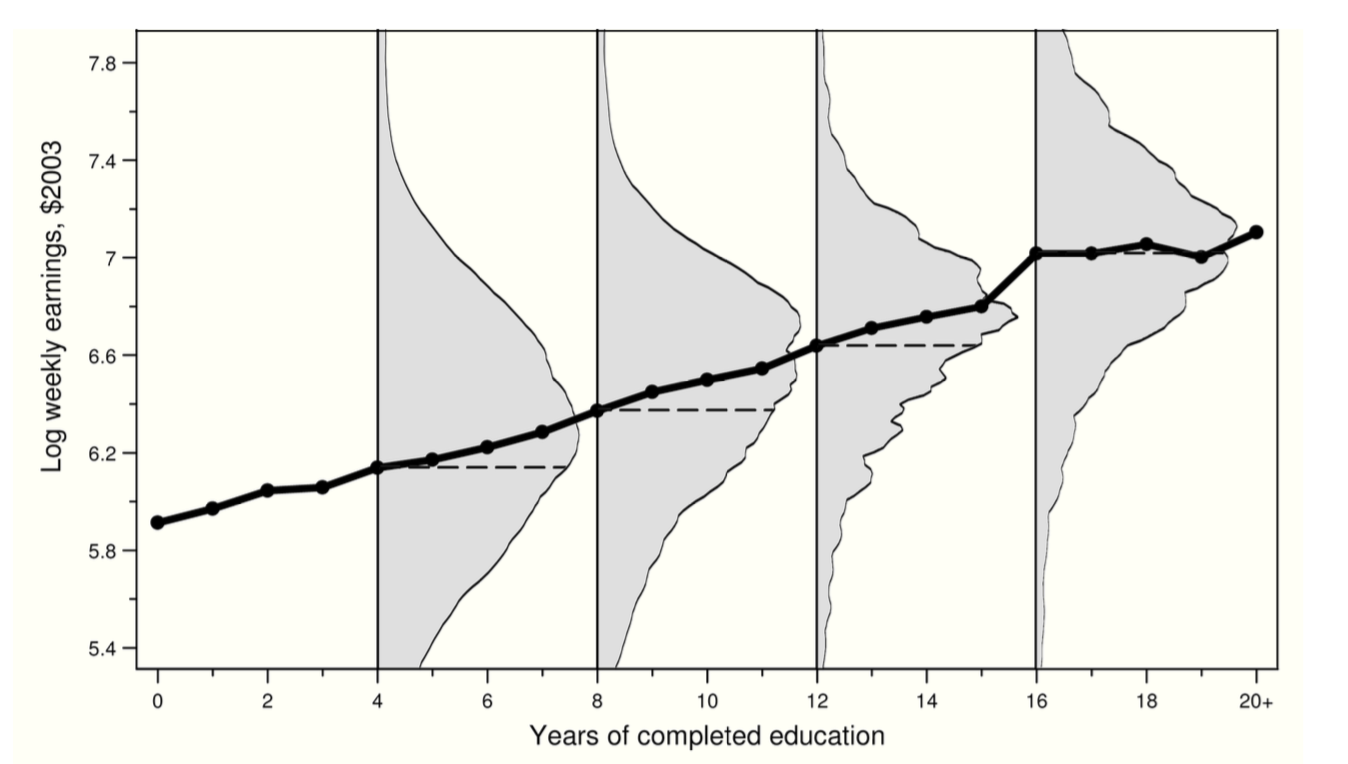
\includegraphics{figures/EarningsEducation}}
%\end{figure}
%
%}
\frame{
%\frametitle{Epstein and Mershon SCOTUS data}

Epstein and Mershon SCOTUS data
\begin{itemize}
\item Data on 27 justices from the Warren, Burger, and Rehnquist courts (can be interpreted as a census)  \pause
\item Percentage of votes in liberal direction for each justice in a number of issue areas  \pause
\item Segal-Cover scores for each justice  \pause
\item Party of appointing president %\pause
%\item We interpret this as having the entire population.
\end{itemize}

}


\frame{
\frametitle{Mean ($\mu$) judicial support for liberal position}

\begin{figure}[ht] \centering
        \scalebox{.4}{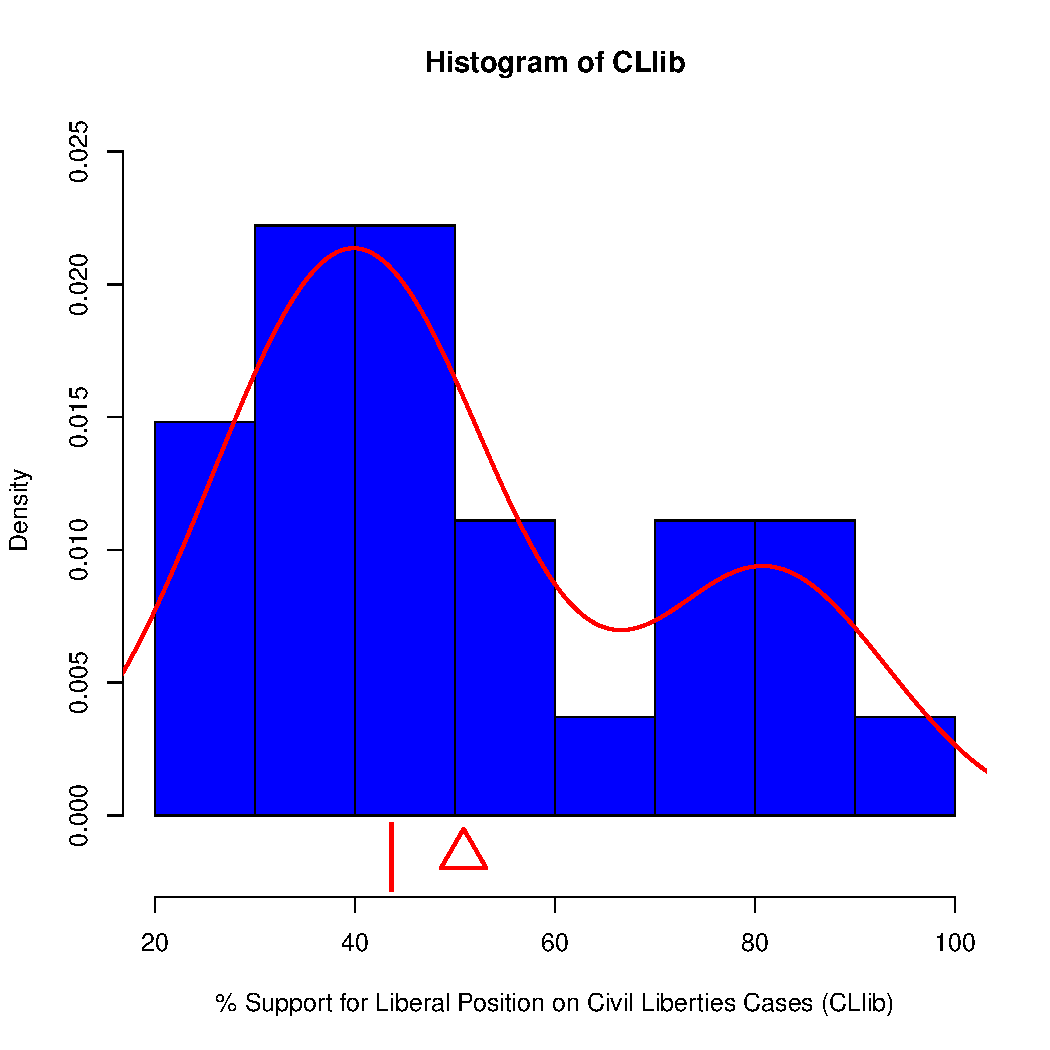
\includegraphics[angle=90,origin=c]{CLhistActSol.pdf}}
\end{figure}

}

\frame{
\frametitle{What are we doing now?}

We will be estimating conditional population parameters ($E[Y|X=x] \approx \beta_0 + \beta_1 x$) and contrasts of population parameters ($E_x (E[Y|X=x+1]-E[Y|X=x]) \approx \beta_1$) from an i.i.d. sample. \\

\bigskip

For example, we will estimate $\beta_1$ with 

{\small
\begin{align*}
\hat{\beta}_{1}&=\frac{\sum_{i=1}^{n}(x_{i1}-\bar{x_{1}})y_{i}}{\sum_{i=1}^{n}(x_{i1}-\bar{x_{1}})^{2}}
\end{align*}
}

and consider properties of this estimator:
\bi
\item Bias
\item Variance
\item Consistency
\item Asymptotic Normality
\ei


}


\frame{
%\frametitle{CLlib Conditional on Party}
CLlib Mean Conditional on Party
\vspace{-.5cm}
\begin{figure}[ht] \centering
        \scalebox{.4}{\includegraphics{figures/partyMean.pdf}}
\end{figure}

}


\frame{
%\frametitle{Linear Conditional Mean Function}
BLP of CLlib

\vspace{-.5cm}
\begin{figure}[ht] \centering
        \scalebox{.4}{
\includegraphics{figures/lmBin.pdf}}
\end{figure}

}

\frame{
%\frametitle{Linear Conditional Mean Function}
BLP of CLlib


\vspace{-.5cm}
\begin{figure}[ht] \centering
        \scalebox{.4}{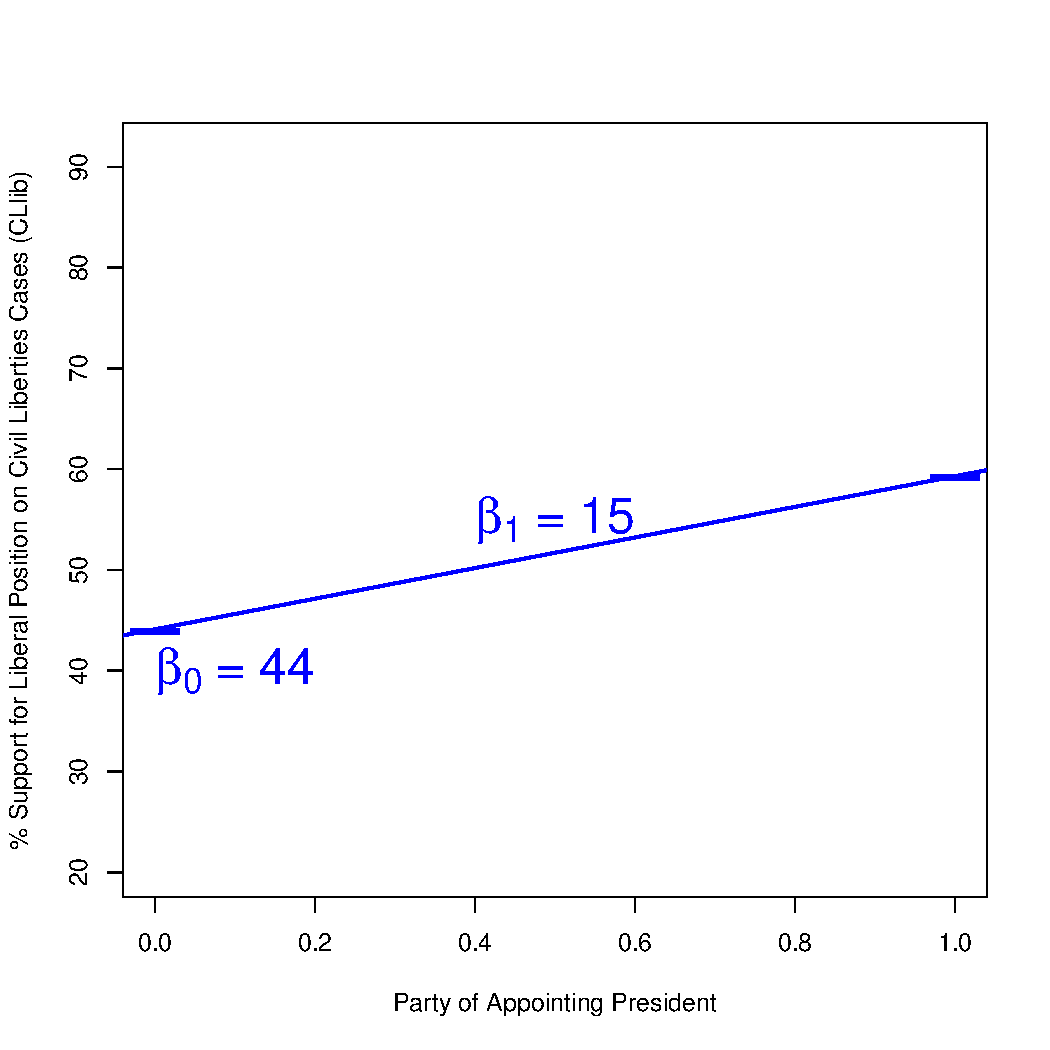
\includegraphics{figures/BinLCEF.pdf}}
\end{figure}

How are the BLP and the CEF related here?
}

\frame{
\frametitle{BLP for CLlib Conditional on SCscore}

\vspace{-.5cm}
\begin{figure}[ht] \centering
        \scalebox{.4}{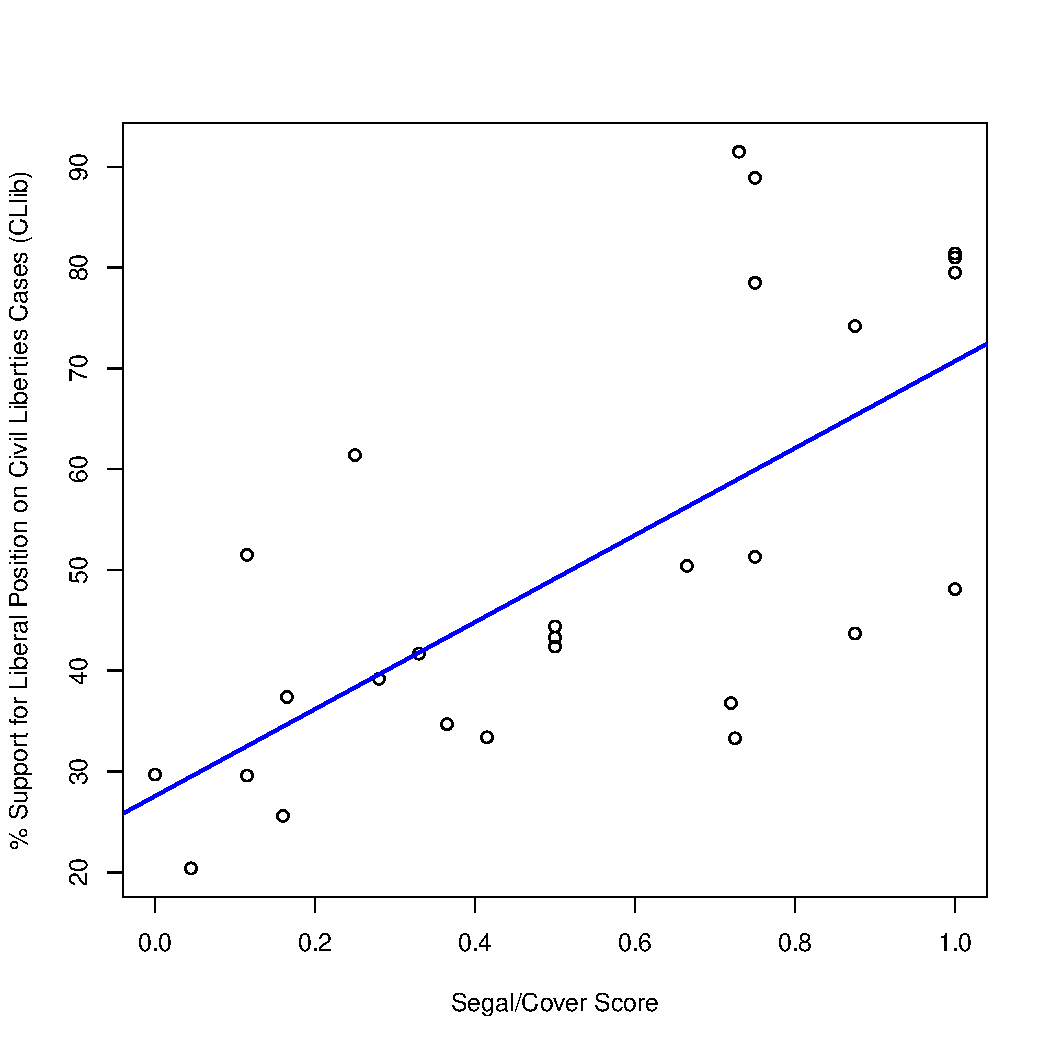
\includegraphics{figures/lm.pdf}}
\end{figure}

}

\frame{
\frametitle{BLP for CLlib Conditional on SCscore}

\vspace{-.5cm}
\begin{figure}[ht] \centering
        \scalebox{.4}{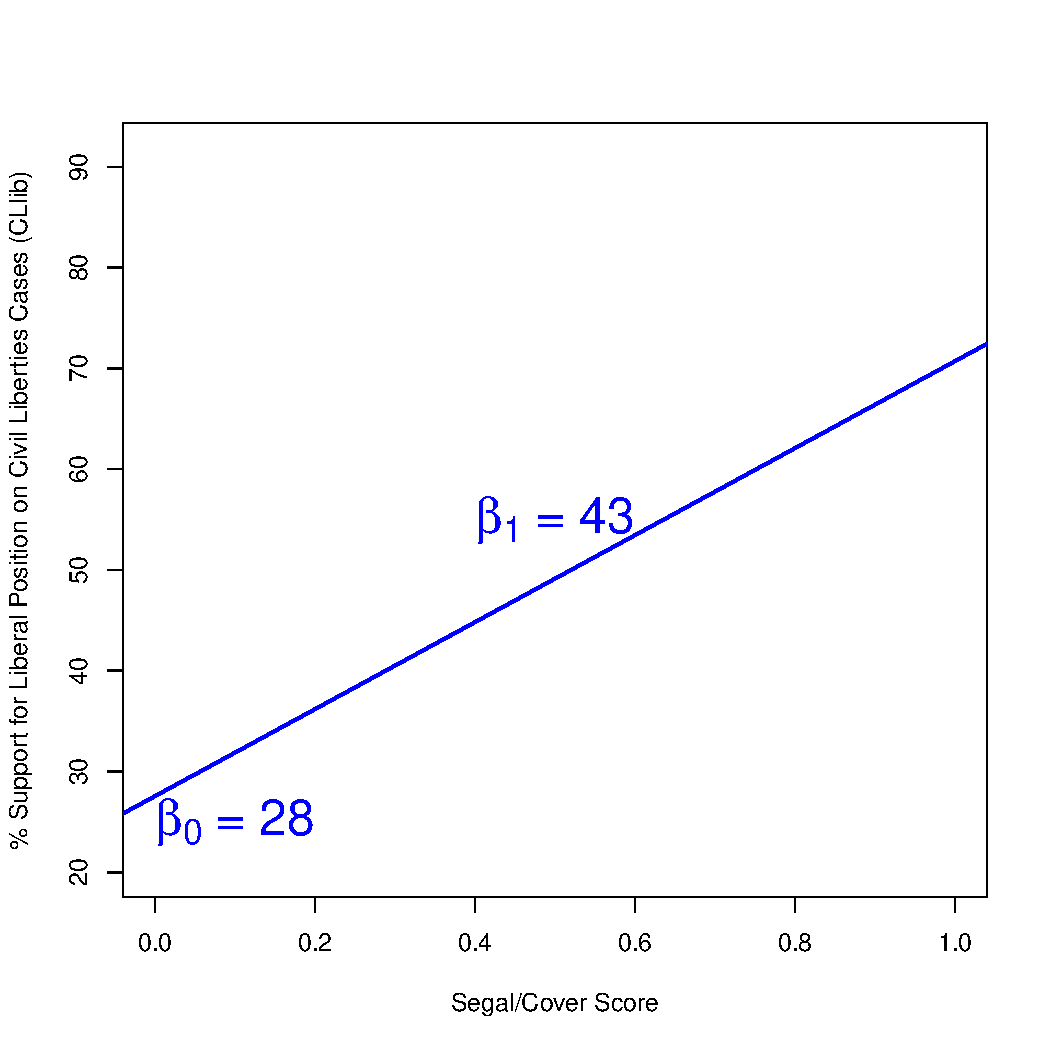
\includegraphics{figures/LCEF.pdf}}
\end{figure}

%How to interpret the intercept and slope descriptively?
}

\frame{

Reminder: where do our estimators come from?

\bi
\item $\hat \mu  = \overline Y$
\item $\hat \sigma_{biased}^2 =\overline Y^2 - \overline{Y}^2$  
\item $\hat \sigma^2 = \frac{n}{n-1}(\overline Y^2 - \overline{Y}^2)$
\ei
\pause

\bigskip
what about 

{\small
\begin{align*}
\hat{\beta}_{1}&=\frac{\sum_{i=1}^{n}(x_{i1}-\bar{x_{1}})y_{i}}{\sum_{i=1}^{n}(x_{i1}-\bar{x_{1}})^{2}}
\end{align*}
}

}

\frame{
\frametitle{Toward a Plug-in Estimator}

The BLP of $Y$ given $X$ is $g(X) = \beta_0 + \beta_1X$, where
$$
\beta_0 = \E[Y] -  \frac{C[X,Y]}{V[X]} \E[X]
$$
and the slope
$$
\beta_1 = \frac{C[X,Y]}{V[X]}.
$$

}

\frame{
\frametitle{Toward a Plug-in Estimator}

The BLP of $Y$ given $X$ is $g(X) = \beta_0 + bX$, where
$$
\beta_0 = \E[Y] -   \frac{\E[XY] - \E[X]\E[Y]}{\E[X^2]-\E[X]^2}   \E[X]
$$
and the slope
$$
\beta_1 = \frac{\E[XY] - \E[X]\E[Y]}{\E[X^2]-\E[X]^2}
$$
}

\frame{

A plug-in {\it estimator} of the BLP:
$$
\hat \beta_0 = \overline{Y} -   \frac{\overline{XY} - \overline{X} \cdot \overline{Y}}{\overline{X^2}-\overline{X}^2}   \overline{X}
$$
and the slope
\begin{align*}
\hat \beta_1 &= \frac{\overline{XY} - \overline{X} \cdot \overline{Y}}{\overline{X^2}-\overline{X}^2} \\
&=\frac{\sum_{i=1}^{n}(x_{i1}-\bar{x_{1}})y_{i}}{\sum_{i=1}^{n}(x_{i1}-\bar{x_{1}})^{2}}
\end{align*}

}

\frame{

Unbiasedness of $\hat \beta_1$ for $\beta_1$


}


\begin{frame}
\begin{itemize}
\item If we write $y_i=\beta_{0}+\beta_{1}x_{1i}+\epsilon_i$. Replace $y_i$. Then,
{\small
\begin{align*}
\hat{\beta}_{1}&=\frac{\sum\limits_{i=1}^{n}(x_{i1}-\bar{x_{1}})y_{i}}{\sum\limits_{i=1}^{n}(x_{i1}-\bar{x_{1}})^{2}}\\
&= \visible<2->{\frac{\sum\limits_{i=1}^{n}(x_{i1}-\bar{x_{1}})(\beta_{0}+\beta_{1}x_{i1}+\epsilon_{i})}{\sum\limits_{i=1}^{n}(x_{i1}-\bar{x_{1}})^{2}}}\\
&=\visible<3->{\frac{\sum\limits_{i=1}^{n}(x_{i1}-\bar{x_{1}})\beta_{0}}{\sum\limits_{i=1}^{n}(x_{i1}-\bar{x_{1}})^{2}}+\frac{\sum\limits_{i=1}^{n}(x_{i1}-\bar{x_{1}})\beta_{1}x_{i1}}{\sum\limits_{i=1}^{n}(x_{i1}-\bar{x_{1}})^{2}}+
\frac{\sum\limits_{i=1}^{n}(x_{i1}-\bar{x_{1}})\epsilon_{i}}{\sum\limits_{i=1}^{n}(x_{i1}-\bar{x_{1}})^{2}}}
%\frac{\sum\limits_{i=1}^{n}(x_{i1}-\bar{x_{1}})\beta_{2}x_{i2}}{\sum\limits_{i=1}^{n}(x_{i1}-\bar{x_{1}})^{2}}}\\
%&\quad\quad\visible<3->{+\frac{\sum\limits_{i=1}^{n}(x_{i1}-\bar{x_{1}})u_{i}}{\sum\limits_{i=1}^{n}(x_{i1}-\bar{x_{1}})^{2}}}
\end{align*}}
\end{itemize}
\end{frame}

\begin{frame}
\begin{itemize}
\item Therefore we have
\begin{align*}
\hat\beta_{1}=\beta_{1}+\frac{\sum\limits_{i=1}^{n}(x_{i1}-\bar{x_{1}})\epsilon_{i}}{\sum\limits_{i=1}^{n}(x_{i1}-\bar{x_{1}})^{2}}
\end{align*}
Take expectation conditional on the all the $x_{i1},i=\dots,n$,
{\scriptsize
\begin{align*}
&E\left[\hat\beta_{1}\vert x_{i1},x_{i2},i=1,\dots,n\right]\\
&=\visible<2->{\beta_{1}+\frac{\sum\limits_{i=1}^{n}(x_{i1}-\bar{x_{1}})E\left[\epsilon_{i}\vert  x_{i1},x_{i2},i=1,\dots,n\right]}{\sum\limits_{i=1}^{n}(x_{i1}-\bar{x_{1}})^{2}}}\\
&=\visible<3->{\beta_{1}  \quad\because Theorem~ 2.2.22}
\end{align*}
}
\end{itemize}
\end{frame}

\frame{

If $E\left[\hat\beta_{1}\vert x_{i1},x_{i2},i=1,\dots,n\right] = \beta_1$,\\
 what is $E[\hat\beta_{1}]$?



}


\frame{
%\frametitle{Linear Conditional Mean Function}
Linear Conditional Mean Function

\vspace{-.5cm}
\begin{figure}[ht] \centering
        \scalebox{.4}{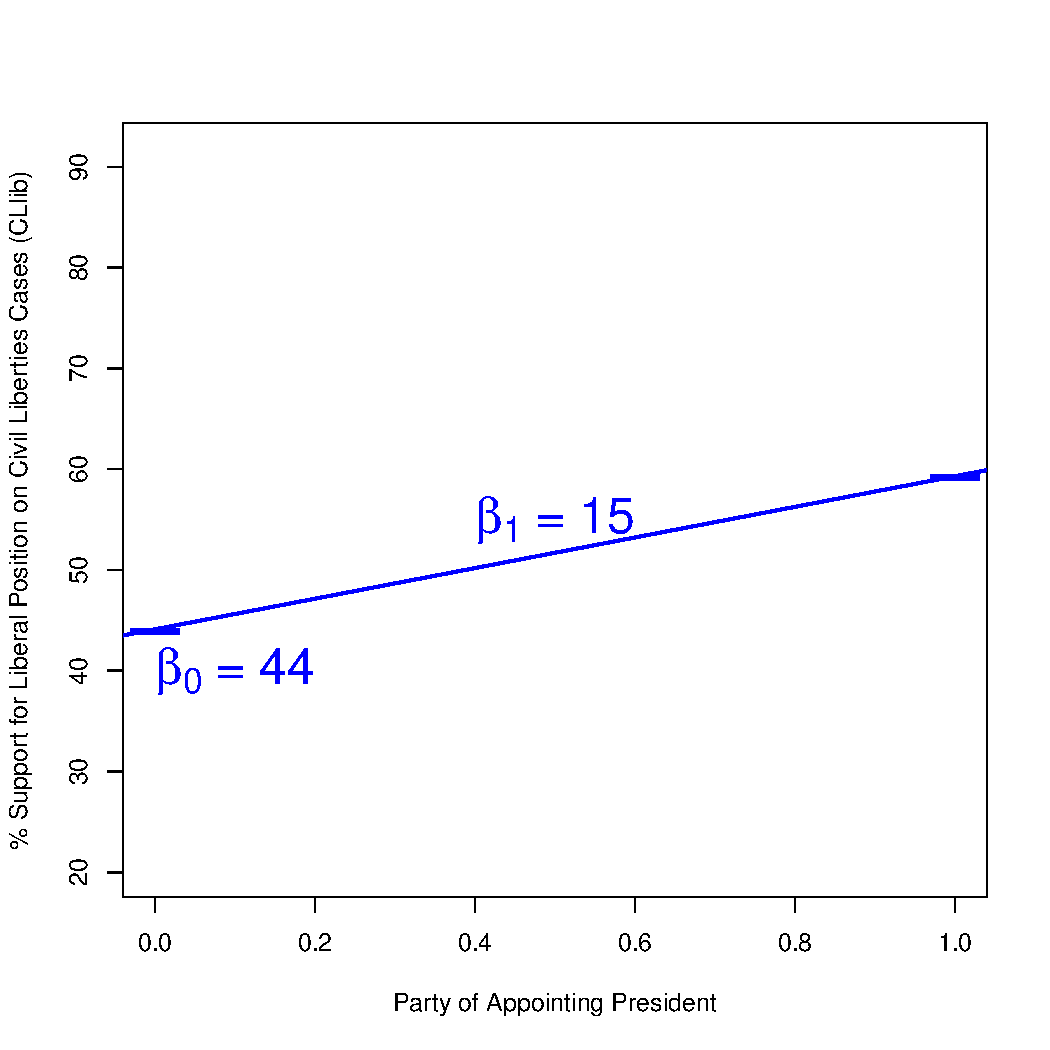
\includegraphics{figures/BinLCEF.pdf}}
\end{figure}

%How to interpret the intercept and slope descriptively?
}

\frame{
%\frametitle{Linear Conditional Expectation Function with Samples}
Linear Conditional Expectation Function with Samples

\begin{center}
\includegraphics<1>[width=3.25in]{figures/BinLCEF.pdf}
\includegraphics<2>[width=3.25in]{figures/BinLCEFsam1.pdf}
\includegraphics<3>[width=3.25in]{figures/BinLCEFsam2.pdf}
\includegraphics<4>[width=3.25in]{figures/BinLCEFsam3.pdf}
\end{center}

}

\frame{
Sampling distribution of the sample slope
\begin{table}[h]
\begin{center}
{\scriptsize
\begin{tabular}{r|r|r|r|r|r|r} %cc
$i$ & \multicolumn{1}{r|}{1} & \multicolumn{1}{r|}{2}   & $\dots$ & \multicolumn{1}{r|}{12} & & \\ % & \multicolumn{1}{c}{$MoE$}& \multicolumn{1}{c}{95\% CI}  \\
$s$  & $Y_1$, $X_1$ & $Y_2$, $X_2$   & $\dots$  & $Y_{12}$,$X_{12}$  & $\hat{\beta}_1$\\ % & $2\cdot\sqrt{\frac{\overline{Y}_{625}(1-\overline{Y}_{625})}{625}}$ & $\overline{Y}_{625} \pm MoE$ \\
\hline
1 & 35,1 & 50,0   & $\dots$  & 22,1 & 14.49   \\ %& \visible<2->{.037} & \visible<3->{[.643,.717]}\\
2 & 28,1 & 19,1   & $\dots$  & 65,0 & 26.21 \\ %& \visible<2->{.037}  & \visible<3->{[.663,.737]}\\
3 & 33,1 & 27,1  & $\dots$  & 45,0 & 9.93 \\ %& \visible<2->{.035} & \visible<3->{[.715,.785]}\\
4 & $\vdots$ & $\vdots$ & $\dots$  & $\vdots$ & $\vdots$ \\ %& \visible<2->{.036} & \visible<3->{[.694,.766]}\\
5 & $\vdots$ & $\vdots$  & $\dots$  & $\vdots$ & $\vdots$ \\ %& \visible<2->{.037} & \visible<3->{[.653,.727]}\\
$\vdots$ & $\vdots$  & $\vdots$ & $\vdots$ & $\vdots$  & $\vdots$ \\ % & \visible<2->{$\vdots$} & \visible<3->{$\vdots$}  \\
\hline
%\visible<1->{$f_{\cdot}(\cdot)$} & \multicolumn{1}{r|}{\visible<1->{?}} & \multicolumn{1}{r|}{\visible<1->{?}}  & $\dots$& \multicolumn{1}{r|}{\visible<1->{?}} & \visible<1->{?} \\
\visible<1->{$\E_{\cdot}(\cdot)$} & \multicolumn{1}{r|}{\visible<1->{50.9, 0.44}} & \multicolumn{1}{r|}{\visible<1->{50.9, 0.44}}  & $\dots$& \multicolumn{1}{r|}{\visible<1->{50.9, 0.44}} & \visible<1->{\textcolor{black}{15}}  \\
%\visible<1->{$V_{\cdot}(\cdot)$} & \multicolumn{1}{r|}{\visible<1->{436}} & \multicolumn{1}{r|}{\visible<1->{436}}  & $\dots$& \multicolumn{1}{r|}{\visible<1->{436}} & \visible<1->{\textcolor{black}{$\frac{436}{12}$}} \\
\end{tabular}}
%\caption{\emph{Sampling Distributions for $\overline{Y}_{625}$, the Margin-of-Error, and the 95\% Confidence Interval}}\label{t:samdistCI}
\end{center}
\end{table}

}


\frame{
\frametitle{Sampling Distributions for $\hat{\beta}_0$ and $\hat{\beta}_1$}

\vspace{-.5cm}
\begin{figure}[ht] \centering
        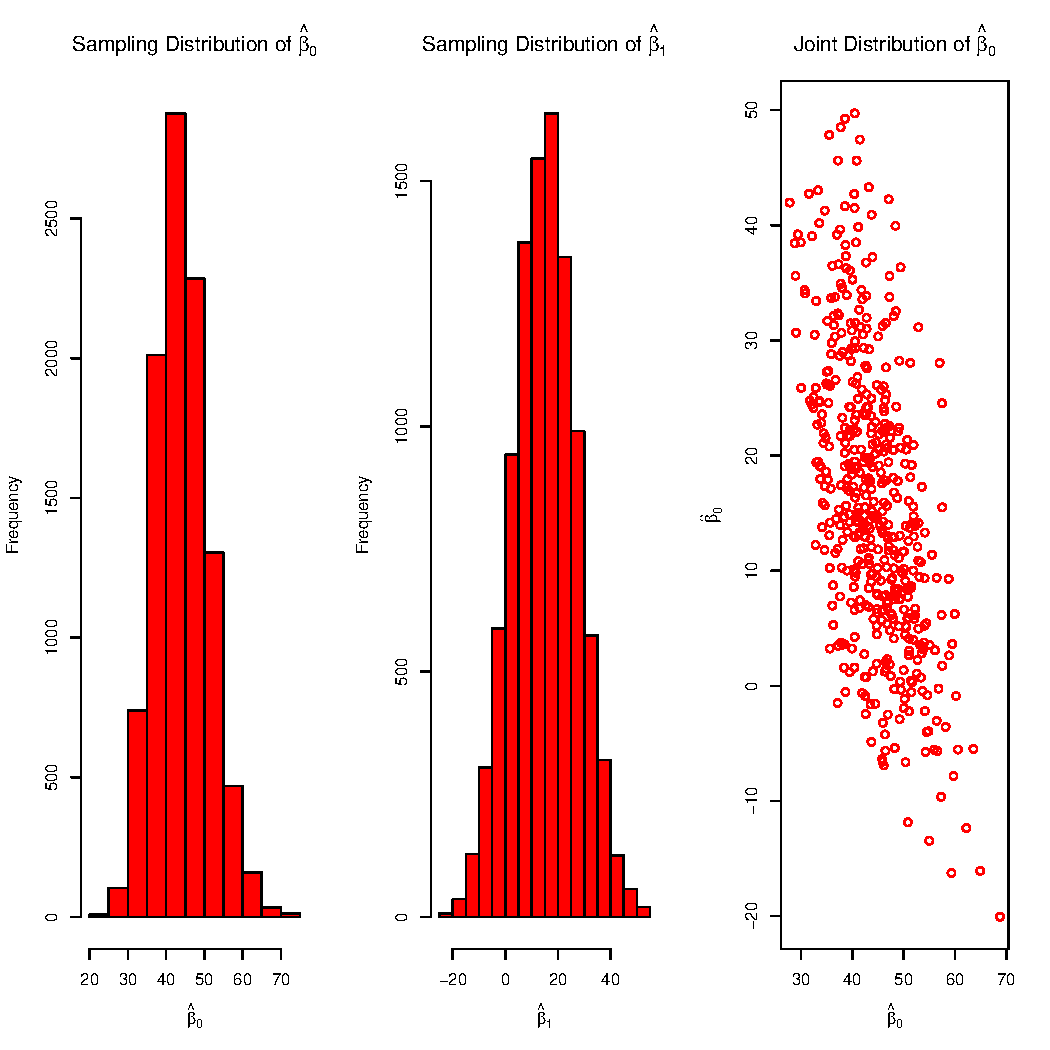
\includegraphics[height=2.5in,width=3.25in]{figures/BinLCEFsamdist.pdf}
\end{figure}

}

%\frame{
%\frametitle{Properties of Point Estimators}

%We would like estimators that are:
%\begin{itemize}
%\item unbiased
%\item low variance
%\item consistent
%\item with known distribution in large samples (often Normal)
%\end{itemize}

%
%}

\frame{
\frametitle{Bias}

\begin{center}
\includegraphics<1>[width=3.25in]{figures/BinLCEFbias1.pdf}
\includegraphics<2>[width=3.25in]{figures/BinLCEFbias2.pdf}
\end{center}

}

\frame{
\frametitle{Assumptions for Unbiasedness}

What assumptions did we need for $E[\hat{\beta}_0]=\beta_0$ and $E[\hat{\beta}_1]=\beta_1$?\\


\vspace{1cm}

\visible<2>{Just random sampling!}


}



\frame{
\frametitle{BLP for CLlib Conditional on SCscore}

\vspace{-.5cm}
\begin{figure}[ht] \centering
        \scalebox{.4}{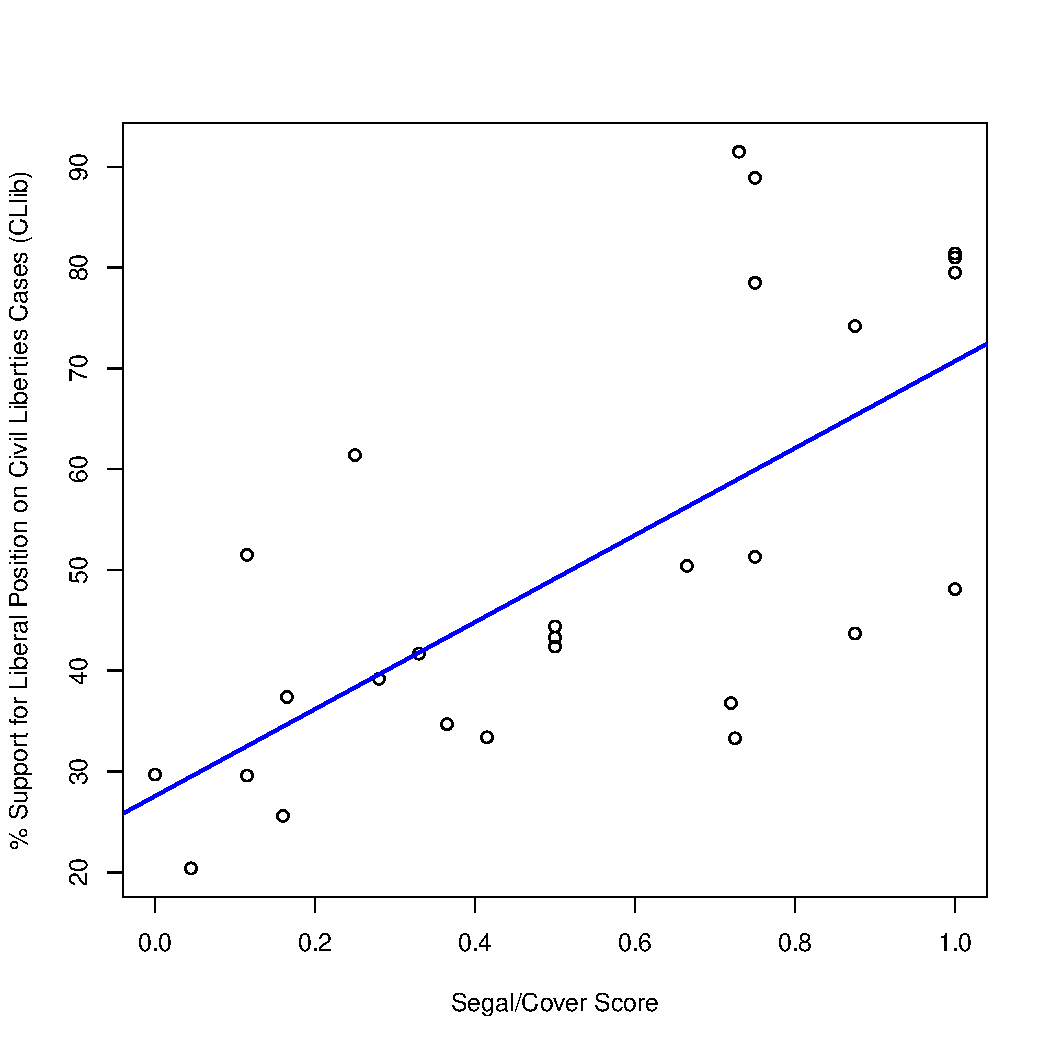
\includegraphics{figures/lm.pdf}}
\end{figure}

}

\frame{
\frametitle{BLP for CLlib Conditional on SCscore}

\vspace{-.5cm}
\begin{figure}[ht] \centering
        \scalebox{.4}{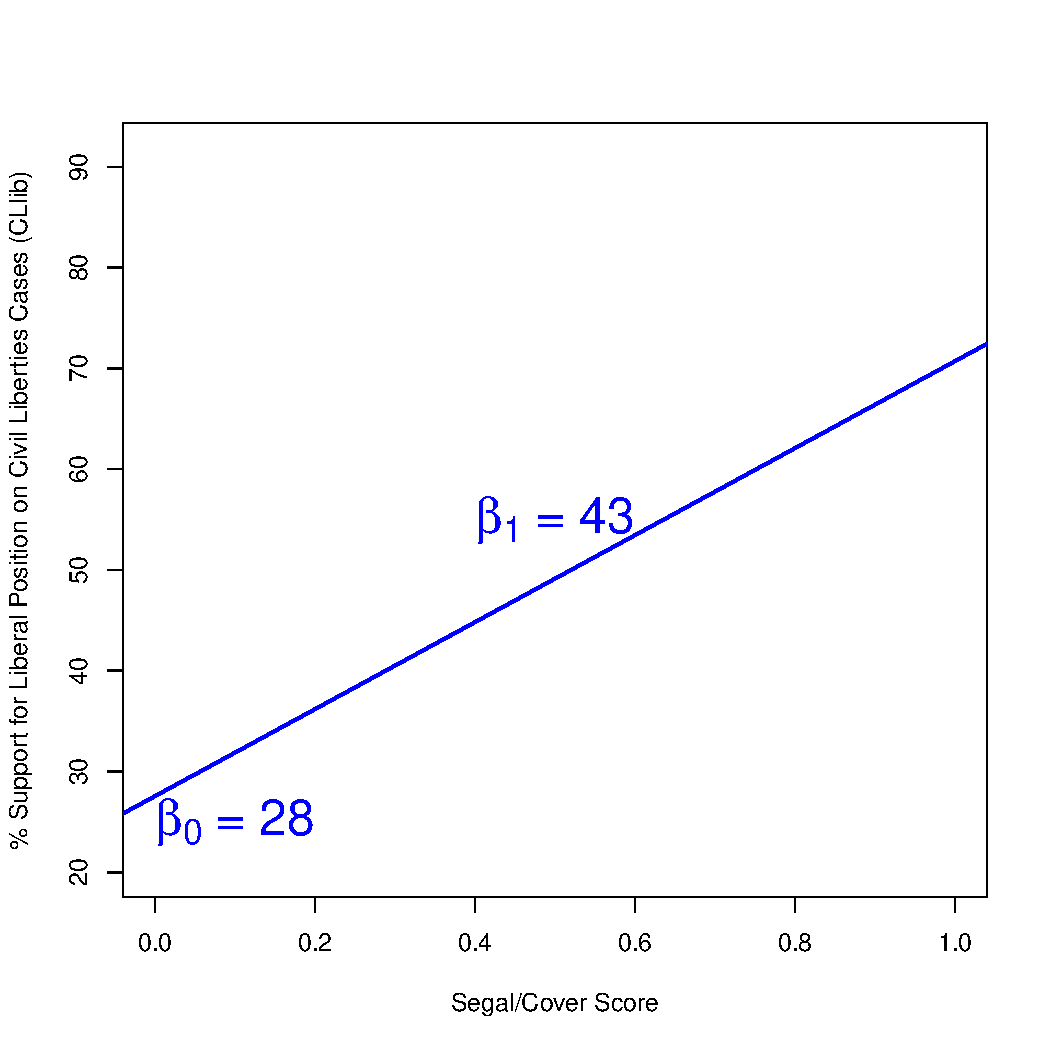
\includegraphics{figures/LCEF.pdf}}
\end{figure}

%How to interpret the intercept and slope descriptively?
}


\frame{
\frametitle{Linear Conditional Expectation Function with Samples}

\begin{center}
\includegraphics<1>[width=3.25in]{figures/LCEF.pdf}
\includegraphics<2>[width=3.25in]{figures/LCEFsam1.pdf}
\includegraphics<3>[width=3.25in]{figures/LCEFsam2.pdf}
\includegraphics<4>[width=3.25in]{figures/LCEFsam3.pdf}
\end{center}

}

\frame{
\frametitle{Sampling Distributions for $\hat{\beta}_0$ and $\hat{\beta}_1$}

\vspace{-.5cm}
\begin{figure}[ht] \centering
        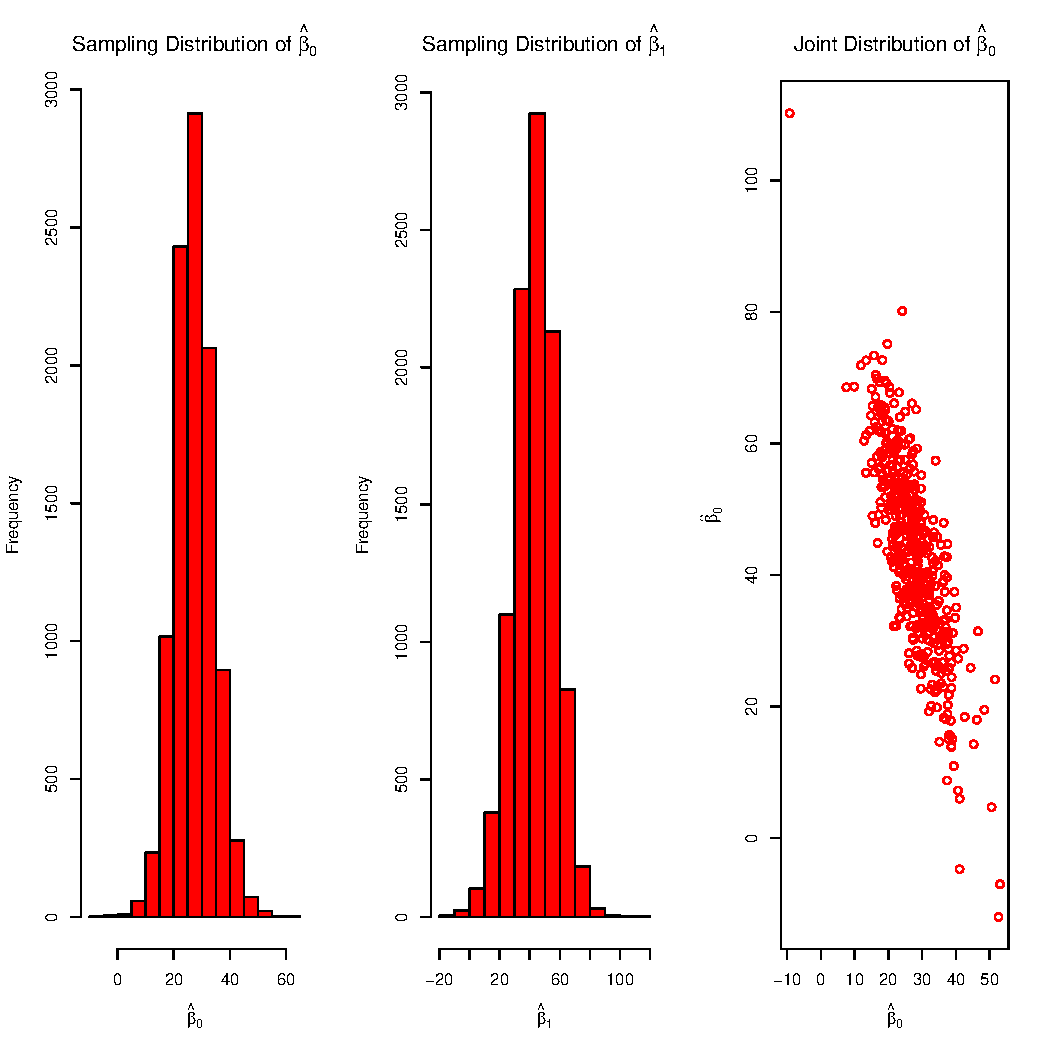
\includegraphics[height=2.5in,width=3.25in]{figures/LCEFsamdist.pdf}
\end{figure}

}

\frame{
\frametitle{Bias}

\begin{center}
\includegraphics<1>[width=3.25in]{figures/LCEFbias1.pdf}
\includegraphics<2>[width=3.25in]{figures/LCEFbias2.pdf}
\end{center}

}

\frame{
\frametitle{Assumptions for Unbiasedness}

What assumptions did we need for $E[\hat{\beta}_0]=\beta_0$ and $E[\hat{\beta}_1]=\beta_1$?\\

\vspace{.3cm}

\visible<2->{Just random sampling!}

\vspace{-.5cm}
\begin{figure}[ht] \centering
        \scalebox{.25}{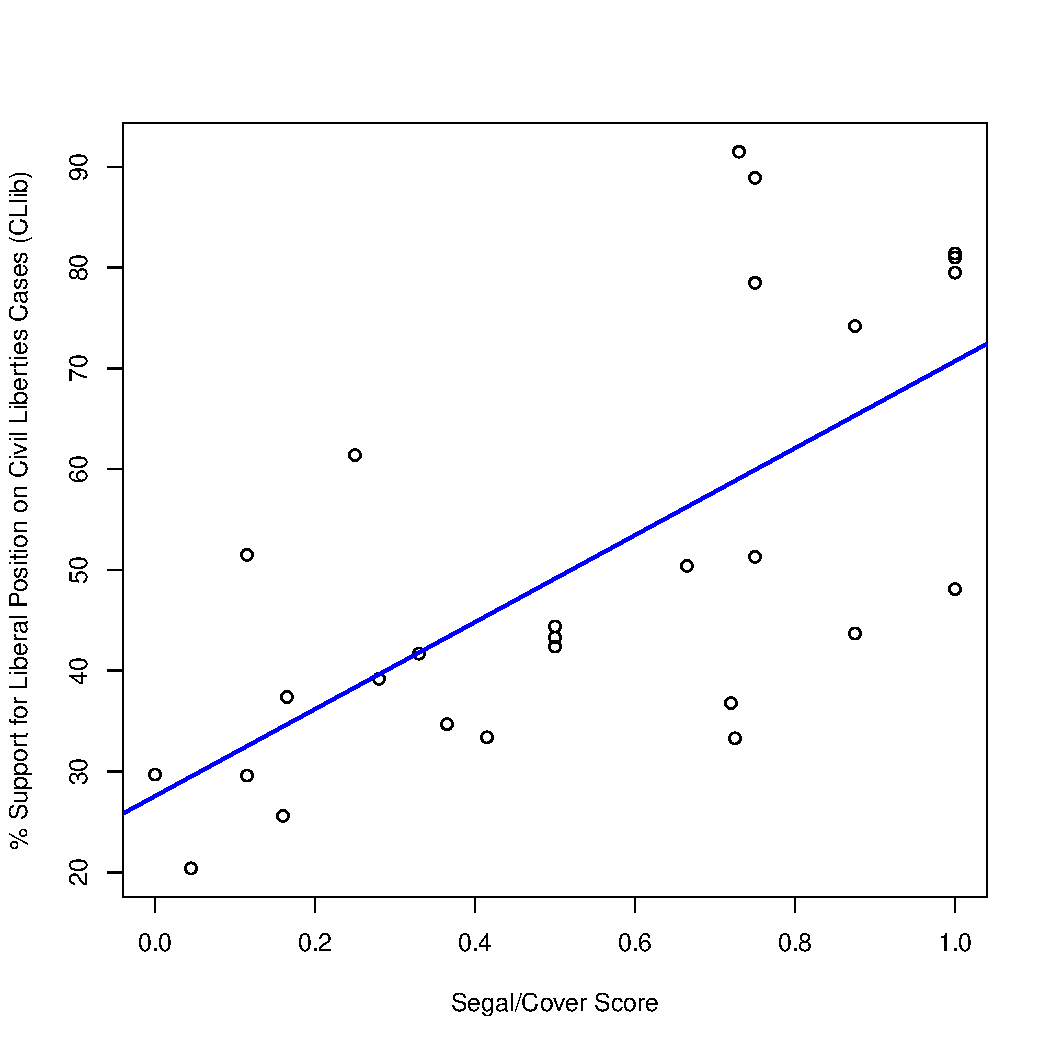
\includegraphics{figures/lm.pdf}}
\end{figure}

\visible<3>{Unless we really wanted to estimate the CEF and not the BLP.}

}









%
%\begin{frame}
%\begin{itemize}
%\item Hence the bias is
%\begin{align*}
%E\left[\hat\beta_{1}\vert x_{i1},x_{i2},i=1,\dots,n\right] -\beta_{1}=\beta_{2}\frac{\sum\limits_{i=1}^{n}(x_{i1}-\bar{x_{1}})x_{i2}}{\sum\limits_{i=1}^{n}(x_{i1}-\bar{x_{1}})^{2}}
%\end{align*}
%%\item The above bias equation suggests us two things. Omitted variable bias would exist if \colorbox{emorygold}{\color{white}(1) $x_{i2}$ is indeed a relevant variable} and \colorbox{emorygold}{\color{white} (2) $x_{i1}$ and $x_{i2}$ are correlated}
%\end{itemize}
%\vspace{4cm}
%\end{frame}


%\frame{
%
%$\hat a$ is the regression estimate of the intercept of the BLP and is consistent for $a$.
%
%\vspace{0.2in}
%
%$\hat b$ is the regression estimate of the slope of the BLP and is consistent for $b$.
%
%}

\frame{

Consistency of $\hat \beta_1$ for $\beta_1$


}

\frame{
\frametitle{Proving consistency of $\hat \beta_1$ for $\beta_1$}

Recall that, 
$$
\beta_1 = \frac{C[X,Y]}{V[X]} = \frac{E[YX]-E[Y]E[X]}{E[X^2]-E[X]^2}
$$

and the plug in estimator is
$$
\hat \beta_1 = \frac{\overline{YX} - \overline Y \cdot  \overline X}{\overline{X^2} - \overline{X}^2}.
$$

Prove consistency. 


}

\frame{

Multivariate Regresssion

}


\frame{

Define
$$
\X = \left( \begin{array}{ccccc} 1 & X_{11} & X_{21} & ... & X_{K1} \\ 1 & X_{12} & X_{22} & ... & X_{K2} \\ \vdots &  \vdots &  \vdots & \ddots &  \vdots \\  1 & X_{1n} & X_{2n} & ... & X_{Kn} \end{array} \right), \hspace{1em}  \Y = \left( \begin{array}{c} Y_1 \\ Y_2 \\ \vdots \\ Y_n \end{array} \right), \hspace{1em}  {\bf e} = \left( \begin{array}{c} e_1 \\  e_2 \\ \vdots \\  e_n \end{array} \right),% {\bf\epsilon} = \left( \begin{array}{c} \epsilon_1 \\  \epsilon_2 \\ \vdots \\  \epsilon_n \end{array} \right),
$$

$$
\text{and} \hspace{1em} \widehat \Beta =\left( \begin{array}{c} \hat \beta_0 \\ \hat \beta_1 \\  \hat \beta_2 \\ \vdots \\ \hat \beta_K \end{array} \right).
 $$
}





\frame{

Then it is equivalent to write the following:
\begin{align*}
Y_1 & = \hat \beta_0 + \hat \beta_1 X_{11} + \hat \beta_2 X_{21} + ... \hat \beta_K X_{K1} + e_1 \\
Y_2 & = \hat \beta_0 + \hat \beta_1 X_{12} + \hat \beta_2 X_{22} + ... \hat \beta_K X_{K2} + e_2 \\
& \qquad \qquad \qquad \quad  ... \\
Y_n & = \hat \beta_0 + \hat \beta_1 X_{1n} + \hat \beta_2 X_{2n} + ... \hat \beta_K X_{Kn} + e_n \\
\end{align*}

}

\frame{

Then it is equivalent to write the following:
\begin{align*}
\left( \begin{array}{c} Y_1 \\ Y_2 \\ \vdots \\ Y_n \end{array} \right) &=  \left( \begin{array}{ccccc} 1 & X_{11} & X_{21} & ... & X_{K1} \\ 1 & X_{12} & X_{22} & ... & X_{K2} \\ \vdots &  \vdots &  \vdots & \ddots &  \vdots \\  1 & X_{1n} & X_{2n} & ... & X_{Kn} \end{array} \right) \left( \begin{array}{c} \hat \beta_0 \\ \hat \beta_1 \\ \hat \beta_2 \\ \vdots \\ \hat \beta_K \end{array} \right) + \left( \begin{array}{c} e_1 \\  e_2 \\ \vdots \\  e_n \end{array} \right).
\end{align*}

}

\frame{

Then it is equivalent to write the following:
\begin{align*}
\Y & = \X \widehat \Beta + {\bf e}.
\end{align*}

}


\frame{
\frametitle{OLS Solution}

$$
\widehat \Beta  = (\X'\X)^{-1} \X' \Y
$$

}

\frame{

Residuals can be written as the following:
\begin{align*}
\left( \begin{array}{c} e_1 \\  e_2 \\ \vdots \\  e_n \end{array} \right) &= \left( \begin{array}{c} Y_1 \\ Y_2 \\ \vdots \\ Y_n \end{array} \right) -  \left( \begin{array}{ccccc} 1 & X_{11} & X_{21} & ... & X_{K1} \\ 1 & X_{12} & X_{22} & ... & X_{K2} \\ \vdots &  \vdots &  \vdots & \ddots &  \vdots \\  1 & X_{1n} & X_{2n} & ... & X_{Kn} \end{array} \right) \left( \begin{array}{c} \hat \beta_0 \\ \hat \beta_1 \\ \hat \beta_2 \\ \vdots \\ \hat \beta_K \end{array} \right).
\end{align*}
\begin{align*}
 {\bf e}  &=  \Y - \X \widehat \Beta.
\end{align*}


}


\frame{

Minimizing the sum of squared residuals:
\begin{align*}
\widehat \Beta = argmin_{\bf b} (\Y - \X \bf{b})' (\Y - \X \bf{b})
\end{align*}

Setting derivatives equal to zero and substituting $\widehat\Beta$ for $\bf b$.
\begin{align*}
2 \X^T (\Y - \X\widehat\Beta)&= 0 \\
\X^T {\bf e} &= 0
\end{align*}

Let's solve the first equation for $\widehat\Beta$.
 
}

\frame{

Recall that $\Y$ can also be written in terms of $\Beta$ and ${\bf \epsilon}$
\begin{align*}
\Y & = \X \Beta + {\bf \epsilon}.
\end{align*}

Let's draw a picture to remind ourselves of the difference between $\widehat\Beta$ and $\Beta$ and  ${\bf e}$ and ${\bf \epsilon}$.

}

\frame{
\frametitle{OLS Solution is Unbiased}

\begin{align*}
\widehat \Beta  &= (\X'\X)^{-1} \X' \Y\\
&= (\X'\X)^{-1} \X' (\X \Beta + {\bf \epsilon}) \\
&= (\X'\X)^{-1} \X'\X \Beta + (\X'\X)^{-1} \X'{\bf \epsilon}) \\
&= \Beta + (\X'\X)^{-1} \X'{\bf \epsilon} \\
\end{align*}

\begin{align*}
E[\widehat \Beta| \X]  &= E[\Beta| \X] + E[(\X'\X)^{-1} \X'{\bf \epsilon}| \X] \\
&= \Beta + (\X'\X)^{-1} \X'E[{\bf \epsilon}| \X] \\
&= \Beta \because Theorem 2.2.22
\end{align*}

}

\frame{

By iterated expectations,

\begin{align*}
E[\widehat \Beta]  &=E_{\X}\{E[\widehat \Beta| \X]  \} \\
&=  E_{\X}\{ \Beta \} \\
&= \Beta
\end{align*}


}

\frame{
\frametitle{Consistency}
$$
\widehat \Beta \rightarrow_p \Beta
$$

\bigskip

Handwaving Proof:
\begin{itemize}
\item Any of the $K$ slopes in $\Beta$ can be rewritten as a simple regression coefficient using the FWL.
\item We've previously shown how to prove the consistency of simple regression coefficients using the LLN and CMT.
\item There are a few details I'm leaving out here. 
\end{itemize}

}

\frame{
Sampling distributions of the simple and multiple sample slopes (in the $X$ direction).
\begin{table}[h]
\begin{center}
{\scriptsize
\begin{tabular}{r|r|r|r|r|r|rr} %cc
$i$ & \multicolumn{1}{r|}{1} & \multicolumn{1}{r|}{2}   & $\dots$ & \multicolumn{1}{r|}{12} & & & \\ % & \multicolumn{1}{c}{$MoE$}& \multicolumn{1}{c}{95\% CI}  \\
$s$  & $Y_1$, $X_1$, $Z_1$ & $Y_2$, $X_2$, $Z_2$   & $\dots$  & $Y_{12}$,$X_{12}$, $Z_{12}$  & $\hat{\beta}_1^s$ & $\hat{\beta}_1^m$\\ % & $2\cdot\sqrt{\frac{\overline{Y}_{625}(1-\overline{Y}_{625})}{625}}$ & $\overline{Y}_{625} \pm MoE$ \\
\hline
1 & 3.3,97,100 & 57.2,36,72.6   & $\dots$  & 39.3,30,40.6 & -.498 & -.499   \\ %& \visible<2->{.037} & \visible<3->{[.643,.717]}\\
2 & 30.4,54,99.3& 54.0,24,28.5  & $\dots$  & 6.2,99,100 & -.456 & -.398 \\ %& \visible<2->{.037}  & \visible<3->{[.663,.737]}\\
3 & 14.7,87,94.8 & 3.8,98,100 & $\dots$  & 3.8,98,100 & -.209 & -.190 \\ %& \visible<2->{.035} & \visible<3->{[.715,.785]}\\
4 & $\vdots$ & $\vdots$ & $\dots$  & $\vdots$ & $\vdots$ \\ %& \visible<2->{.036} & \visible<3->{[.694,.766]}\\
5 & $\vdots$ & $\vdots$  & $\dots$  & $\vdots$ & $\vdots$ \\ %& \visible<2->{.037} & \visible<3->{[.653,.727]}\\
$\vdots$ & $\vdots$  & $\vdots$ & $\vdots$ & $\vdots$  & $\vdots$ \\ % & \visible<2->{$\vdots$} & \visible<3->{$\vdots$}  \\
\hline
%\visible<1->{$f_{\cdot}(\cdot)$} & \multicolumn{1}{r|}{\visible<1->{?}} & \multicolumn{1}{r|}{\visible<1->{?}}  & $\dots$& \multicolumn{1}{r|}{\visible<1->{?}} & \visible<1->{?} \\
\visible<1->{$\E_{\cdot}(\cdot)$} & \multicolumn{1}{r|}{\visible<1->{17.3, 70.7,89.3}} & \multicolumn{1}{r|}{\visible<1->{17.3, 70.7,89.3}}  & $\dots$& \multicolumn{1}{r|}{\visible<1->{17.3, 70.7,89.3}} & \visible<1->{\textcolor{black}{-.52}} & -.33  \\
%\visible<1->{$V_{\cdot}(\cdot)$} & \multicolumn{1}{r|}{\visible<1->{436}} & \multicolumn{1}{r|}{\visible<1->{436}}  & $\dots$& \multicolumn{1}{r|}{\visible<1->{436}} & \visible<1->{\textcolor{black}{$\frac{436}{12}$}} \\
\end{tabular}}
%\caption{\emph{Sampling Distributions for $\overline{Y}_{625}$, the Margin-of-Error, and the 95\% Confidence Interval}}\label{t:samdistCI}
\end{center}
\end{table}

}




\begin{frame}{Omitted Variable Bias}

\begin{itemize}

\item Suppose the model you've estimated is
\begin{align*}
y_{i}=\beta_{0}+\beta_{1}x_{i1}+u_{i}
\end{align*}
when the model you wanted was
\begin{align*}
y_{i}=\beta_{0}+\beta_{1}x_{i1}+\beta_{2}x_{i2}+u_{i}
\end{align*}

\end{itemize}
\end{frame}

\begin{frame}

\begin{itemize}
\item Then your OLS estimator, $\hat{\beta}_{1}$ is

{\small
\begin{align*}
\hat{\beta}_{1}&=\frac{\sum\limits_{i=1}^{n}(x_{i1}-\bar{x_{1}})y_{i}}{\sum\limits_{i=1}^{n}(x_{i1}-\bar{x_{1}})^{2}}
\end{align*}
}

\item Use the rules of conditional expectation to derive the bias.
\end{itemize}
\end{frame}
\begin{frame}
\begin{itemize}
\item Recall that the model we wanted was $y_i=\beta_{0}+\beta_{1}x_{1i}+\beta_{2}x_{2i}+u_i$. Replace $y_i$. Then,
{\small
\begin{align*}
\hat{\beta}_{1}&=\frac{\sum\limits_{i=1}^{n}(x_{i1}-\bar{x_{1}})y_{i}}{\sum\limits_{i=1}^{n}(x_{i1}-\bar{x_{1}})^{2}}\\
&= \visible<2->{\frac{\sum\limits_{i=1}^{n}(x_{i1}-\bar{x_{1}})(\beta_{0}+\beta_{1}x_{i1}+\beta_{2}x_{i2}+u_{i})}{\sum\limits_{i=1}^{n}(x_{i1}-\bar{x_{1}})^{2}}}\\
&=\visible<3->{\frac{\sum\limits_{i=1}^{n}(x_{i1}-\bar{x_{1}})\beta_{0}}{\sum\limits_{i=1}^{n}(x_{i1}-\bar{x_{1}})^{2}}+\frac{\sum\limits_{i=1}^{n}(x_{i1}-\bar{x_{1}})\beta_{1}x_{i1}}{\sum\limits_{i=1}^{n}(x_{i1}-\bar{x_{1}})^{2}}+\frac{\sum\limits_{i=1}^{n}(x_{i1}-\bar{x_{1}})\beta_{2}x_{i2}}{\sum\limits_{i=1}^{n}(x_{i1}-\bar{x_{1}})^{2}}}\\
&\quad\quad\visible<3->{+\frac{\sum\limits_{i=1}^{n}(x_{i1}-\bar{x_{1}})u_{i}}{\sum\limits_{i=1}^{n}(x_{i1}-\bar{x_{1}})^{2}}}
\end{align*}}
\end{itemize}
\end{frame}
\begin{frame}
\begin{itemize}
\item Therefore we have
\begin{align*}
\hat\beta_{1}=\beta_{1}+\beta_{2}\frac{\sum\limits_{i=1}^{n}(x_{i1}-\bar{x_{1}})x_{i2}}{\sum\limits_{i=1}^{n}(x_{i1}-\bar{x_{1}})^{2}}+\frac{\sum\limits_{i=1}^{n}(x_{i1}-\bar{x_{1}})u_{i}}{\sum\limits_{i=1}^{n}(x_{i1}-\bar{x_{1}})^{2}}
\end{align*}
Take expectation conditional on the all the $x_{i1},x_{i2},i=\dots,n$,
{\scriptsize
\begin{align*}
&E\left[\hat\beta_{1}\vert x_{i1},x_{i2},i=1,\dots,n\right]\\
&=\visible<2->{\beta_{1}+\beta_{2}\frac{\sum\limits_{i=1}^{n}(x_{i1}-\bar{x_{1}})x_{i2}}{\sum\limits_{i=1}^{n}(x_{i1}-\bar{x_{1}})^{2}}+\frac{\sum\limits_{i=1}^{n}(x_{i1}-\bar{x_{1}})E\left[u_{i}\vert  x_{i1},x_{i2},i=1,\dots,n\right]}{\sum\limits_{i=1}^{n}(x_{i1}-\bar{x_{1}})^{2}}}\\
&=\visible<3->{\beta_{1}+\beta_{2}\frac{\sum\limits_{i=1}^{n}(x_{i1}-\bar{x_{1}})x_{i2}}{\sum\limits_{i=1}^{n}(x_{i1}-\bar{x_{1}})^{2}} }% \quad\because MLR4
\end{align*}
}
\end{itemize}
\end{frame}

\begin{frame}
\begin{itemize}
\item Hence the bias is
\begin{align*}
E\left[\hat\beta_{1}\vert x_{i1},x_{i2},i=1,\dots,n\right] -\beta_{1}=\beta_{2}\frac{\sum\limits_{i=1}^{n}(x_{i1}-\bar{x_{1}})x_{i2}}{\sum\limits_{i=1}^{n}(x_{i1}-\bar{x_{1}})^{2}}
\end{align*}
%\item The above bias equation suggests us two things. Omitted variable bias would exist if \colorbox{emorygold}{\color{white}(1) $x_{i2}$ is indeed a relevant variable} and \colorbox{emorygold}{\color{white} (2) $x_{i1}$ and $x_{i2}$ are correlated}
\end{itemize}
\vspace{4cm}
\end{frame}


\frame{
\frametitle{Multivariate OVB}

\begin{itemize}

\item Suppose the model you've estimated is
\begin{align*}
\Y= \X\Beta + \epsilon
\end{align*}
when the model you wanted was
\begin{align*}
\Y= \X\Beta + \Z\Delta + \epsilon
\end{align*}


\end{itemize}
}

\frame{

Define
$$
\X = \left( \begin{array}{ccccc} 1 & X_{11} & X_{21} & ... & X_{K1} \\ 1 & X_{12} & X_{22} & ... & X_{K2} \\ \vdots &  \vdots &  \vdots & \ddots &  \vdots \\  1 & X_{1n} & X_{2n} & ... & X_{Kn} \end{array} \right), \hspace{1em}   \Beta =\left( \begin{array}{c} \beta_0 \\ \beta_1 \\ \beta_2 \\ \vdots \\ \beta_K \end{array} \right),
$$

$$
\Z = \left( \begin{array}{cccc}  Z_{11} & Z_{21} & ... & Z_{J1} \\  Z_{12} & Z_{22} & ... & Z_{J2} \\  \vdots &  \vdots & \ddots &  \vdots \\  Z_{1n} & Z_{2n} & ... & Z_{Jn} \end{array} \right), \hspace{1em}  
 \Delta =\left( \begin{array}{c}  \delta_1 \\  \delta_2 \\ \vdots \\  \delta_J \end{array} \right).
$$

%$$
%\text{and} \hspace{1em} \Beta =\left( \begin{array}{c} \beta_0 \\ \beta_1 \\ \beta_2 \\ \vdots \\ \beta_K \end{array} \right).
% $$
 
 $$
  \Y = \left( \begin{array}{c} Y_1 \\ Y_2 \\ \vdots \\ Y_n \end{array} \right), \hspace{1em}  {\bf\epsilon} = \left( \begin{array}{c} \epsilon_1 \\  \epsilon_2 \\ \vdots \\  \epsilon_n \end{array} \right).
 $$
 
}


\begin{frame}

\begin{itemize}
\item Then your OLS estimator, $\hat{\Beta}$ is

{\small
\begin{align*}
\left[\X^T \X \right]^{-1} \X^T \Y & = \hat \Beta  \\
\left[\X^T \X \right]^{-1} \X^T [\X \Beta + \Z\Delta + {\bf\epsilon}] & = \hat \Beta \\
\left[\X^T \X \right]^{-1} \X^T \X \Beta + \left[\X^T \X \right]^{-1} \X^T \Z \Delta + \left[\X^T \X \right]^{-1} \X^T {\bf\epsilon} & = \hat \Beta \\
\Beta + \left[\X^T \X \right]^{-1} \X^T \Z \Delta + \left[\X^T \X \right]^{-1} \X^T {\bf\epsilon} & = \hat \Beta
\end{align*}
}

\item Use the rules of conditional expectation to derive the bias.
\end{itemize}
\end{frame}

\frame{




{\small
\begin{align*}
\E[\Beta + \left[\X^T \X \right]^{-1} \X^T \Z \Delta + \left[\X^T \X \right]^{-1} \X^T {\bf\epsilon}] & = \E[ \hat \Beta | \X,\Z] \\
\Beta + \left[\X^T \X \right]^{-1} \X^T \Z \Delta + \left[\X^T \X \right]^{-1} \X^T \E[{\bf\epsilon}| \X,\Z] & = \E[ \hat \Beta | \X,\Z] \\
\Beta + \left[\X^T \X \right]^{-1} \X^T \Z \Delta  & = \E[ \hat \Beta | \X,\Z]
\end{align*}
}
}


\frame{
\frametitle{Example with $K=2$ and $J=1$ }


{\small
\begin{align*}
Z_1 &=\X \Gamma  + \nu \\
&= \left( \begin{array}{ccc} 1 & X_{11} & X_{21}  \\ 1 & X_{12} & X_{22}  \\ \vdots   & \ddots &  \vdots \\  1 & X_{1n} & X_{2n}  \end{array} \right)  \left( \begin{array}{c} \hat \gamma_0 \\ \hat \gamma_1 \\ \hat \gamma_2 \end{array} \right)   + \left( \begin{array}{c} \nu_1 \\  \nu_2 \\ \vdots \\  \nu_n \end{array} \right) %\\
%&= \left( \begin{array}{c} \hat \gamma_0 \\ \hat \gamma_1 \\ \hat \gamma_2 \end{array} \right) 
 \end{align*}
}

 {\small
\begin{align*}
 \left[\X^T \X \right]^{-1} \X^T \Z \Delta  & =   \left[\X^T \X \right]^{-1} \X^T Z_1  \cdot   \delta_1 \\
 & =   \hat \Gamma  \cdot   \delta_1 \\
 & =   \left( \begin{array}{c} \hat \gamma_0 \\ \hat \gamma_1 \\ \hat \gamma_2 \end{array} \right) \cdot   \delta_1 \\
 \end{align*}
}

\center

Bias for $\beta_1$ is $\hat \gamma_1 \cdot   \delta_1$

}

\frame{
\frametitle{Example with $K=2$ and $J=2$ (Part 1)}


{\small
\begin{align*}
Z_1 &=\X \Gamma^1  + \nu^1 \\
&= \left( \begin{array}{ccc} 1 & X_{11} & X_{21}  \\ 1 & X_{12} & X_{22}  \\ \vdots   & \ddots &  \vdots \\  1 & X_{1n} & X_{2n}  \end{array} \right)  \left( \begin{array}{c} \hat \gamma_0^1 \\ \hat \gamma_1^1 \\ \hat \gamma_2^1 \end{array} \right)   + \left( \begin{array}{c} \nu_1^1 \\  \nu_2^1 \\ \vdots \\  \nu_n^1 \end{array} \right) %\\
%&= \left( \begin{array}{c} \hat \gamma_0 \\ \hat \gamma_1 \\ \hat \gamma_2 \end{array} \right) 
 \end{align*}
}

{\small
\begin{align*}
Z_2 &=\X \Gamma^2  + \nu^2 \\
&= \left( \begin{array}{ccc} 1 & X_{11} & X_{21}  \\ 1 & X_{12} & X_{22}  \\ \vdots   & \ddots &  \vdots \\  1 & X_{1n} & X_{2n}  \end{array} \right)  \left( \begin{array}{c} \hat \gamma_0^2 \\ \hat \gamma_1^2 \\ \hat \gamma_2^2 \end{array} \right)   + \left( \begin{array}{c} \nu_1^2 \\  \nu_2^2 \\ \vdots \\  \nu_n^2 \end{array} \right) %\\
%&= \left( \begin{array}{c} \hat \gamma_0 \\ \hat \gamma_1 \\ \hat \gamma_2 \end{array} \right) 
 \end{align*}
}

}

\frame{
\frametitle{Example with $K=2$ and $J=2$ (Part 2)}



 {\small
\begin{align*}
 \left[\X^T \X \right]^{-1} \X^T \Z \Delta  & =   \left[\X^T \X \right]^{-1} \X^T Z_1  \cdot   \delta_1 +\left[\X^T \X \right]^{-1} \X^T Z_2  \cdot   \delta_2 \\
& =   \left( \begin{array}{c} \hat \gamma_0^1 \\ \hat \gamma_1^1 \\ \hat \gamma_2^1 \end{array} \right) \cdot   \delta_1 +  \left( \begin{array}{c} \hat \gamma_0^2 \\ \hat \gamma_1^2 \\ \hat \gamma_2^2 \end{array} \right) \cdot   \delta_2 \\
 \end{align*}
}

\center

Bias for $\beta_1$ is $\hat \gamma_1^1 \cdot   \delta_1 + \hat \gamma_1^2 \cdot   \delta_2$

}







\frame{
\frametitle{Why do we care about SEs?}


%\begin{itemize}
%\item If x has been randomized, what do we know about the slope in the x direction for OLS with x and OLS with x and z?
%\item<2-> Write the estimated classical SE formulas for OLS with x and OLS with x and z, where x has been randomized.
%%\item Sampling distribution table for OLS with x and OLS with x and z, where x has been randomized
%%\item Include formulas for SEs (or variances) and discuss bias and efficiency (including VIF and changing errors) and draw sampling distributions
%%\item Discuss estimation of $\sigma^2$ for different models (similarities and differences).
%%\item Present SE for heteroskedasticity with single x, and prove equals classic SE when homoskedasticity holds
%%\item Discuss data transformation version of WLS and include in table and discussion and draw sampling distributions.
%\end{itemize}

\begin{itemize}
\item<2-> Inference (e.g., confidence intervals)
\item<3-> Efficiency (i.e., lower MSE)
\end{itemize}



%\visible<4>{Compare sampling distributions for OLS with one and two vars, WLS?, and Estimators of SEs on the board}

}


\frame{
\frametitle{How to make CIs}

Two main ideas:
\begin{enumerate}
\item<1-> Normal Approximation
\begin{enumerate}
\item<2-> prove asymptotic normality of estimator
\item<3-> derive mean and variance (and SE) of estimator (why only these needed?)
\item<4-> estimate components of variance (and bias if necessary)
\item<5-> do the CI algebra
\end{enumerate}
\item<6-> Bootstrap
\end{enumerate}

}

\frame{

We can decompose the $\hat\Beta$ into the expected value and the sampling error.

\begin{align*}
\left[\X^T \X \right]^{-1} \X^T \Y & = \hat \Beta  \\
\left[\X^T \X \right]^{-1} \X^T [\X \Beta + {\bf\epsilon}] & = \hat \Beta \\
\left[\X^T \X \right]^{-1} \X^T \X \Beta + \left[\X^T \X \right]^{-1} \X^T {\bf\epsilon} & = \hat \Beta \\
\Beta + \left[\X^T \X \right]^{-1} \X^T {\bf\epsilon} & = \hat \Beta
\end{align*}

}
%
%\frame{
%
%\begin{align*}
%\left[\X^T \X \right]^{-1} \X^T \Y & = \hat \beta  \\
%\left[\X^T \X \right]^{-1} \X^T [\X \beta + {\bf\epsilon}] & = \hat \beta \\
%\left[\X^T \X \right]^{-1} \X^T \X \beta + \left[\X^T \X \right]^{-1} \X^T {\bf\epsilon} & = \hat \beta \\
%\beta + \left[\X^T \X \right]^{-1} \X^T {\bf\epsilon} & = \hat \beta
%\end{align*}
%
%}

\frame{

Thus:

\begin{align*}
 V\left[\hat \Beta\right] &= V\left[\Beta + \left[\X^T \X \right]^{-1} \X^T {\bf\epsilon}\right] \\
&= V\left[\left[\X^T \X \right]^{-1} \X^T {\bf\epsilon}\right]
\end{align*}


}


%\frame{
%
%By Slutsky's Theorem,
%
%\begin{align*}
%n V\left[\hat \Beta\right] &\arrowp n V\left[\left[\E[\X^T \X] \right]^{-1} \X^T {\bf\epsilon}\right] \\
%& = n \left[\E[\X^T \X] \right]^{-1} V\left[ \X^T {\bf\epsilon}\right] \left[\E[\X^T \X] \right]^{-1} \\
%& = n \left[\E[\X^T \X] \right]^{-1} \E\left[ \X^T \text{diag}[{\bf\epsilon}^2] \X \right] \left[\E[\X^T \X] \right]^{-1}
%\end{align*}
%
%The idea is that we can characterize the sampling variability of the estimator just by characterizing the relationship between the errors and the predictors.
%
%}

\frame{

Estimation: plug in residuals. This is the ``sandwich estimator."

\begin{align*}
\hat V\left[\hat \Beta\right] & = \left[\X^T \X \right]^{-1}  \X^T
 {\text{diag}} \left[ (\Y - \X\hat\Beta)^2 \right]
  \X \left[\X^T \X \right]^{-1}.
\end{align*}

This uses the residuals to {\it estimate} the relationship between the $X$ variables and the errors.

\vspace{0.2in}

%N.b., the errors are {\it in expectation} zero. Analogously, the residuals are by definition {\it on average} zero. Otherwise we could improve the fit by changing the constant. C.f., the MMSE approximation.

}

\frame{

One note: there are many variants of the variance estimators, that involve premultiplying by, e.g., $\frac{n}{n-K}$ or $\frac{n}{n-K-2}$, etc. These are analogous to the unbiased sample variance vs. plug-in sample variance. It's not so simple with the robust variance estimators (many variants: HC0, HC1, HC2) but they all have the same probability limit.

}


\frame{

There is an alternative. ``Classical" variance estimation. If we {\it assume} that $V[\epsilon | X_1, X_2, ..., X_K] = \sigma^2$ for all values of $X_1, X_2, ..., X_K$: homoskedasticity. Then:

\begin{align*}
n V\left[\hat \Beta\right] &\arrowp  n \left[\E[\X^T \X] \right]^{-1} \E\left[ \X^T \text{diag}[{\bf\epsilon}^2] \X \right] \left[\E[\X^T \X] \right]^{-1} \\
&= n  \sigma^2 \left[\E[\X^T \X] \right]^{-1} \E\left[ \X^T \I \X \right] \left[\E[\X^T \X] \right]^{-1} \\
&= n  \sigma^2 \left[\E[\X^T \X] \right]^{-1} \E\left[ \X^T \X \right] \left[\E[\X^T \X] \right]^{-1} \\
&= n  \sigma^2 \left[\E[\X^T \X] \right]^{-1}
 \end{align*}

Where $ \sigma^2 = V [\epsilon] = \E[\epsilon^2]$.

}

%\frame{
%
%There is an alternative. ``Classical" variance estimation. If we {\it assume} that $V[\epsilon | X_1, X_2, ..., X_K] = \sigma^2$ for all values of $X_1, X_2, ..., X_K$: homoskedasticity. Then:
%
%\begin{align*}
%n V\left[\hat \beta\right] &\arrowp  n \left[\E[\X^T \X] \right]^{-1} \E\left[ \X^T {\bf\epsilon} {\bf\epsilon}^T \X \right] \left[\E[\X^T \X] \right]^{-1} \\
%&= n  \sigma^2 \left[\E[\X^T \X] \right]^{-1} \E\left[ \X^T \X \right] \left[\E[\X^T \X] \right]^{-1} \\
%&= n  \sigma^2 \left[\E[\X^T \X] \right]^{-1}
% \end{align*}
%
%Where $ \sigma^2 = V [\epsilon] = \E[\epsilon^2]$.
%
%}

%\frame{
%
%There is an alternative. ``Classical" variance estimation. If we {\it assume} that $V[\epsilon | X_1, X_2, ..., X_K] = \sigma^2$ for all values of $X_1, X_2, ..., X_K$: homoskedasticity. Then:
%
%\begin{align*}
%\hat V\left[\hat \Beta\right] &= \hat \sigma^2 \left[\X^T \X \right]^{-1}.
% \end{align*}
%
%Where $\hat \sigma^2 = \hat V [\Y - \X\hat\Beta]$.
%
%}


\frame{

Classical standard errors make an additional assumption: the magnitude of the errors is {\it unrelated} to the values of the $X$s.

\vspace{0.1in}

This assumption is unlikely to hold. Usually -- in real life -- the errors will be ``heteroskedastic," because in real life, data is messy. If homoskedasticity {\it does} hold, then in large samples, the classical and ``robust" variance estimates will agree.

\vspace{0.1in}

With large $n$ and i.i.d. sampling, always use robust standard errors or bootstrapping to characterize the uncertainty of your regression fit.

%\vspace{0.1in}
%
%What do constant treatment effects imply about homo/heteroskedasticity? What kind of test does the contrapositive allow for?

}


\frame{
If $Y$ and $X$ have been centered and $x$ is a nonstochastic scalar (everything works basically the same if we relax non-stochastic assumption)

\begin{align*}
 V\left[\hat \Beta\right] &= V\left[\Beta +\left[    \frac{\sum_i x_i {\bf\epsilon}_i}{\sum_i x_i^2}\right] \right] \\
 &=    \frac{ V\left[\sum_i x_i {\bf\epsilon}_i\right] }{\left[\sum_i x_i^2\right]^2 } \\
%&=E_x V\left[\left[ \frac{ X_i {\bf\epsilon}_i}{\sum_i X_i^2}\right]
\end{align*}



How does this further simplify if homoskedasticity?

%\vsf
%
%What are the plug-in estimators for these?

}

%\frame{
%\frametitle{Adding variables}
%
%On board draw sampling distribution tables and formulas:
%
%\begin{itemize}
%\item one explanatory var
%\item two explanatory vars
%\end{itemize}
%}






\frame{
Bootstrapping
\begin{enumerate}
\item Take a sample of size n with replacement from your sample
\item Calculate $\beta^{(s=1)}$ from that bootstrap sample
\item Repeat for $s=1,...S$ where $S$ is big
\item  Do one of the following:
\begin{itemize}
\item Calculate bootstrapped variance $\frac{1}{S-1} \sum_{s=1}^S (\beta^{(s)} - \overline{\beta^{(s)}})^2$
\item Put $\{\beta^{(s)}: s=1,...,S\}$ in order and report the $\alpha/2$ and $1-\alpha/2$ percentiles
\item ...
\end{itemize}
\end{enumerate}

\vsf

Takes care of heteroskedasticity automatically.
}


\frame{
\frametitle{Standard Errors/Variance (with homoskedasticity)}

With homoskedasticity, the simple regression model can be written as:

\begin{align*}
 y_i &= \beta_0^s + \beta_1^s x_i + \epsilon_i^s \\
 V&[\epsilon_i]  = \sigma^2_s
\end{align*}

and the two covariate multiple regression model can be written as:

\begin{align*}
 y_i &= \beta_0^m + \beta_1^m x_i + \beta_1^m z_i + \epsilon_i^m \\
 V&[\epsilon_i^m]  = \sigma^2_m
\end{align*}


}


\frame{
\frametitle{Comparing variances (with homoskedasticity)}


\begin{align*}
V[\hat \beta_1^s] &= \frac{\sigma^2_s}{\sum_{i=1}^n (x_i - \bar x)^2 }  \\
V[\hat \beta_1^m] &= \frac{1}{1-R^2_{x \sim z}} \cdot \frac{\sigma^2_m}{\sum_{i=1}^n (x_i - \bar x)^2 } 
\end{align*} \pause

\bigskip

If $x$ is randomized, then what does that tell us about

\bi
\item $\beta_1^s$ and $\beta_1^m$
\item $V[\hat \beta_1^s]$ and $V[\hat \beta_1^m]$
\ei


}


\frame{

November 1

}




\frame{
\frametitle{Linear Models: what are they good for?}

Linear Models
\begin{enumerate}
\item Easy to fit
\item Easy to interpret
\item Nice properties (e.g., FWL)
\item Easy SE formulas
\item Easy sensitivity analysis (later)
\end{enumerate}\pause

\bigskip

Non-linear Models
\begin{enumerate}
\item Easy to fit? (yep, computers)
\item Easy to interpret? (kind of, computers)
\item Nice properties (some, BDC later)
\item Easy SE formulas? (no, but bootstrapping)
\item Easy sensitivity analysis? (later) \pause
\item Robust? (yep, computers and cross-validation)
\end{enumerate}


}


\frame{

What if the CEF is nonlinear?

\vspace{0.2in}

I.e., what if $\E[Y | X] \neq a + bX$?

\vspace{0.2in}

Can we still use linear regression?

}
%
%
%\frame{
%
%Today, I will detail the bivariate case.
%
%}
%
\frame{

Suppose the data were generated:
$$
Y = 10 X^2 + U,
$$
where $X$ is distributed $Uniform(0,1)$ and $U$ is distributed $Normal(0,1)$.


}
\frame{

The CEF is nonlinear $\E[Y | X] = 10 X^2$. But what would the BLP be?

}

\frame{

Draw Figure 4.3.1 on board.

}


%\frame{
%
%\begin{center}
%%\includegraphics[width=0.75\textwidth]{nonlin1.PDF}
%
%\end{center}
%}
%
%\frame{
%
%\begin{center}
%%\includegraphics[width=0.75\textwidth]{nonlin2.PDF}
%
%\end{center}
%}
%
%\frame{
%
%The CEF is nonlinear $\E[Y | X] = 10 X^2$. But what would the BLP be?
%
%}
%
%\frame{
%
%\begin{center}
%%\includegraphics[width=0.75\textwidth]{nonlin3.PDF}
%
%\end{center}
%}

\frame{

BLP is a good, but not great approximation to the CEF. Can we do better with OLS?

}

\frame{

Suppose now we created a second variable: $X^2$. Then we want to estimate:
$$
\argmin_{\beta_0, \beta_1, \beta_2} \E (Y - \beta_0 - \beta_1 X - \beta_2 X^2)^2.
$$
The {\it best linear predictor} with respect to $X$ and $X^2$ is the CEF here!

}

\frame{
\begin{center}
BLP = CEF = $\E[Y | X, X^2]$ = $\E[Y | X]$ =
$
 \beta_0 +  \beta_1  X + \beta_2 X^2.
$
\end{center}
}


\frame{
\begin{center}
BLP = CEF = $\E[Y | X^2]$ =  $\E[Y | X]$ =
$
 0 +  0  X + 10 X^2.
$
\end{center}
}



\frame{

When the CEF is linear in $X$, $X^2$,

 $$ \E[Y | X] = \beta_0 + \beta_1 X + \beta_2 X^2.$$

}

\frame{

When the CEF is not linear in $X$, $X^2$,

 $$ \E[Y | X] \approx \beta_0 + \beta_1 X + \beta_2 X^2.$$

}


\frame{
How to interpret slopes?

\vspace{0.2in}

Before: linear estimate of slope of CEF was $\beta_1$.

\vspace{0.2in}

How can we generalize?

}

\frame{

When the CEF is linear in $X$, $X^2$,

$$\frac{\partial \E[Y | X]}{\partial X} = \frac{\partial (\beta_0 +  \beta_1  X + \beta_2 X^2)}{\partial X}$$

}

\frame{

When the CEF is linear in $X$, $X^2$,

$$\frac{\partial \E[Y | X]}{\partial X} = \beta_1 + 2 \beta_2 X$$

}

\frame{

When the CEF is linear in $X$, $X^2$,

$$\frac{\partial \E[Y | X]}{\partial X} = \beta_1 + 2 \beta_2 X$$

\vspace{0.2in}

The slope of the CEF depends on the value of $X$.

}

\frame{

When the CEF is linear in $X$, $X^2$,

$$\frac{\partial \E[Y | X]}{\partial X} = \beta_1 + 2 \beta_2 X$$

\vspace{0.2in}
with
$$
g(x) = \beta_0 + \beta_1 x + \beta_2 x^2.
$$
what is

$$g(x+1/2)-g(x-1/2)$$

}


%
%
%\frame{
%
%\begin{center}
%%\includegraphics[width=0.75\textwidth]{nonlin2.PDF}
%
%\end{center}
%}
%
%%\frame{
%%
%%When the CEF is not linear in $X$, $X^2$,
%%
%%$$\frac{\partial \E[Y | X]}{\partial X} \approx \beta_1 + 2 \beta_2 X$$
%%
%%}
%
%\frame{
%
%Can we develop a general result for approximating the CEF with polynomials?
%
%}
%
\frame{

Can we develop a general result for approximating the CEF with polynomials? (Yes!)

}

\frame{

The Weierstrass approximation theorem:

\vspace{0.2in}

Any continuous function defined on a closed interval can be uniformly approximated to arbitrary precision using a polynomial function.

}



\frame{

Let's visualize this. Let's take a complex CEF:

$$
\E[Y| X = x] = \left\{
     \begin{array}{lr}
       0 & : x \in [-1,0] \\
       x^2  & : x  \in (0,1) \\
       2 - x & x  \in [1,3]
     \end{array}
   \right.
$$

}

\frame{
\frametitle{Overfitting}

Draw Figures 4.3.4 and 4.3.5 from book

}
%
%\frame{
%
%\begin{center}
%%\includegraphics[width=0.75\textwidth]{poly.PDF}
%\end{center}
%}
%
%\frame{
%
%Let's approximate the CEF with polynomials of $X$.
%
%}
%
%%\frame{
%%
%%\begin{center}
%%\includegraphics[width=0.75\textwidth]{poly1.PDF}
%%\end{center}
%%}
%%\frame{
%%
%%\begin{center}
%%\includegraphics[width=0.75\textwidth]{poly2.PDF}
%%\end{center}
%%}
%%\frame{
%%
%%\begin{center}
%%\includegraphics[width=0.75\textwidth]{poly3.PDF}
%%\end{center}
%%}
%%\frame{
%%
%%\begin{center}
%%\includegraphics[width=0.75\textwidth]{poly4.PDF}
%%\end{center}
%%}
%%\frame{
%%
%%\begin{center}
%%\includegraphics[width=0.75\textwidth]{poly5.PDF}
%%\end{center}
%%}
%%
%%\frame{
%%
%%\begin{center}
%%\includegraphics[width=0.75\textwidth]{poly10.PDF}
%%\end{center}
%%}
%
%\frame{
%
%I am not saying that it is good practice to include a polynomial of length 10!
%
%\vspace{0.2in}
%
%But the point holds. We can always approximate the CEF to arbitrary precision, as long as it's continuous -- even when it's not smooth [i.e., differentiable]!
%
%}
%
%\frame{
%
%When we think about regression as a way to estimate expected values, we see that linearity doesn't matter -- it can be arbitrarily relaxed.
%
%}
%
%
%\frame{
%
%To formalize a bit. Suppose $\E[Y | x]$ is continuous and $\Supp(X) = [a,b]$, then for any positive $\epsilon$ and for all integers $K' \geq K$, there always exists a $K$ such that:
%$$
%\E\left[ \left(\E[Y | x] - \left(\beta_0 + \beta_1 x + \beta_2 x^2 + ... + \beta_{K'} x^{K'}\right)\right)^2\right] < \epsilon,
%$$
%where the $\beta_k$s denote the BLP coefficients with respect to $(1,X,X^2,...,X^{K'})$ . Proof follows from Weierstrass and MMSE properties of the BLP.
%
%}

%\frame{
%
%To formalize a bit. Suppose $\E[Y | x]$ is continuous and $\Supp(X) = [a,b]$, then for any positive $\epsilon$ and for all integers $K' \geq K$, there always exists a $K$ such that:
%$$
%\E\left[ \left(\E[Y | x] - \sum_{k=0}^{K} \beta_k\right)^2\right] < \epsilon,
%$$
%where the $\beta_k$s denote the BLP coefficients with respect to $(1,X,X^2,...,X^{K'})$ . Proof follows from Weierstrass and MMSE properties of the BLP.
%
%}
%
%
%%\frame{
%%
%%To formalize a bit. For continuous $\E[Y | x]$, then for any positive $\epsilon$, there always exists a $K$, such that:
%%$$
%%\E[ \E[Y | x] - \left(\beta_0 + \beta_1 x + \beta_2 x^2 + ... + \beta_K x^K\right))^2] < \epsilon,
%%$$for all values of $x \in [a,b]$.
%%
%%}
%
%\frame{
%
%So as long as you're willing to be sufficiently flexible in how you write out your regressors, you can always do a pretty good job approximating the CEF.
%
%\vspace{0.2in}
%
%So if you're worried about the linearity in linear regression, you can relax it without much issue. Polynomials are just one way [high-order polynomials are not a particularly good way, for rather complicated reasons]. In the next class, I will detail others.
%
%}
%
%\frame{
%
%Example from book.
%
%}

%\frame{
%
%See overfitting example from book, but what about a more formal criteria.
%
%}
%
%\frame{
%\frametitle{Bias/Var Tradeoff}
%
%Recall the estimators:
%\begin{align*}
%\overline{Y^2} -&  \overline{Y}^2 \\
%\frac{n}{n-1}[\overline{Y^2} -&  \overline{Y}^2]
%\end{align*}
%
%Compare the two on bias and variance.
%
%}
%
%\frame{
%
%Go to regression bias/variance tradeoff example
%
%}


\frame{

What about multiple $X$:
\begin{itemize}
\item Additive, Interactive, and Saturated Models
\item with polynomials
\item What if not linear in $\beta$?
%\item statistical/machine learning approaches
\end{itemize}

}


%
%\frame{
%
%[Looking at data.]
%
%}
%
%\frame{
%
%Next class: discrete regressors, interaction terms, saturated models.
%
%}
%
%
%\frame{
%
%Nonlinearity in the CEF, part II.
%
%\vspace{0.2in}
%
%(Or: if you can't find a way to do it with linear regression, you probably shouldn't be doing it.)
%
%}
%
%\frame{
%
%How we'll proceed today:
%\begin{itemize}
%\item Interactions between variables
%\item Binary regressors
%\item Saturated models
%\item Real example: QOG data
%\end{itemize}
%
%}
%
%\frame{
%
%Last class, I showed that, with polynomials, we could arbitrarily approximate any sort of nonlinearity in CEF in one variable.
%
%\vspace{0.2in}
%
%In many ways, this was a proof of concept. This principle generalizes to the multivariate case.
%
%}
%
\frame{

What happens when the conditional slope of the CEF with respect to $X_1$ depends on the value of $X_2$?

\vspace{0.2in}

The BLP is still the BLP, but we might be missing out on an interesting {\it interaction} between the variables $X_1$ and $X_2$.

}

\frame{

So, to formalize a bit, what if the CEF is otherwise linear, but includes an {\it interaction}?
$$
\E[Y  | X_1, X_2] = \beta_0 + \beta_1 X_1 + \beta_2 X_2 + \beta_3 X_1 X_2
$$

}


\frame{

Much as before, we could derive the slope of the CEF with respect to a given variable.
$$
\frac{\partial \E[Y  | X_1, X_2]}{\partial X_1} = \frac{\partial \beta_0 + \beta_1 X_1 + \beta_2 X_2 + \beta_3 X_1 X_2}{\partial X_1}.
$$

}


\frame{

Much as before, we could derive the slope of the CEF with respect to a given variable.
$$
\frac{\partial \E[Y  | X_1, X_2]}{\partial X_1} = \beta_1 + \beta_3 X_2.
$$

}


\frame{

$$
\frac{\partial \E[Y  | X_1, X_2]}{\partial X_1} = \beta_1 + \beta_3 X_2.
$$

The conditional slope of the CEF with respect to $X_1$ {\it depends on the value} of $X_2$.

}





%%
%%\frame{
%%
%%$$
%%\frac{\partial \E[Y  | X_1, X_2]}{\partial X_1} = \beta_1 + \beta_3 X_2.
%%$$
%%
%%The conditional slope of the CEF with respect to $X_1$ {\it depends on the value} of $X_2$.
%%
%%}
%
%\frame{
%
%How to read the coefficients then? If the CEF is linear in $X_1$, $X_2$ and $X_1 X_2$,
%
%$$
%\E[Y  | X_1, X_2] = \beta_0 + \beta_1 X_1 + \beta_2 X_2 + \beta_3 X_1 X_2
%$$
%
%\begin{itemize}
%\item $\beta_0$ is the value of $\E[Y  | X_1 = 0, X_2=0]$.
%\item $\beta_1$ is the slope of the CEF w.r.t. $X_1$ when $X_2 = 0$.
%\item $\beta_2$ is the slope of the CEF w.r.t. $X_2$ when $X_1 = 0$.
%\item $\beta_3$ is how each of the slopes changes, when you move one unit in the other variable
%\begin{itemize}
%\item I.e., if $X_2$ moves from $0$ to $1$, then the slope of the CEF w.r.t. $X_1$ changes by $\beta_3$.
%\item I.e., if $X_1$ moves from $4$ to $7$, then the slope of the CEF w.r.t. $X_2$ changes by $3 \beta_3$.
%\end{itemize}
%\end{itemize}
%
%}
%
%\frame{
%
%How to read the coefficients then? If the CEF is linear in $X_1$, $X_2$ and $X_1 X_2$,
%
%$$
%\E[Y  | X_1, X_2] = \beta_0 + \beta_1 X_1 + \beta_2 X_2 + \beta_3 X_1 X_2
%$$
%
%\vspace{0.2in}
%
%If $\beta_3 = 0$, then $\E[Y  | X_1, X_2] = \beta_0 + \beta_1 X_1 + \beta_2 X_2$, and the interaction is irrelevant.
%
%}
%
\frame{

For full generality, interactions can be combined with polynomials, e.g.:
$$
\E[Y  | X_1, X_2] = \beta_0 + \beta_1 X_1 + \beta_2 X_2 + \beta_3 X_1 X_2 + \beta_4 X_2^2 + \beta_5 X_1^2 X_2
$$

With slopes computed by taking partial derivatives.

\bigskip

Let's find

$$
\frac{\partial \E[Y|\X]}{\partial X_1}|_{\X=x}
$$


}
%
%\frame{
%
%In general, what's the easiest way to interpret?
%
%\vspace{0.2in}
%
%Just compute the implied $\E[Y | X_1, X_2]$ for different values of $X_1$, $X_2$. You can always interpret the coefficients straightforwardly.
%
%}
%
%\frame{
%
%Again, linear regression (OLS) yields a consistent estimate of the $\beta$s for any of the above specifications.
%
%\vspace{0.2in}
%
%Recall: when the CEF is not linear in the defined variables, you're just estimating the features of the BLP. I.e., it's a good principled guess of the CEF.
%
%}
%
%%\frame{
%%
%%Remember: the CEF characterizes the expected value of $Y$ given certain values of $X_1$ and $X_2$.
%%
%%\vspace{0.2in}
%%
%%The ``regular" BLP approximates the CEF, in part, but ruling out the idea that conditional slopes depend on
%%
%%}
%
%
%%
%%\frame{
%%
%%Remember when we derived the expected value, $\E[Y]$, as the MMSE approximation to the unconditional distribution of $Y$?
%%
%%}
%
%
%\frame{
%
%So don't worry about nonlinearity for linear regression.
%\begin{itemize}
%\item It ``usually" doesn't matter all that much for our substantive interpretation.
%\item It can always be relaxed arbitrarily.
%\end{itemize}
%
%}
%
%\frame{
%
%I'm going to discuss a couple more points to reinforce these ideas.
%
%}
%

\frame{
\frametitle{Average Partial Derivative}

The partial derivative can differ for all possible $\X=x$
$$
\frac{\partial \E[Y|\X]}{\partial X_1}|_{\X=x}
$$

Often, we will be interested in an average of these partials

$$
APD_{X_1} = E\left[ \frac{\partial \E[Y|\X]}{\partial X_1}|_{\X=x} \right]
$$
 
where the average is taken over the distribution of $\X$.

}

\frame{
\frametitle{Estimated Average Partial Derivative}

In practice, we just average over the partials at the data points
$$
\widehat{APD}_{X_1} = \frac{1}{n}\sum_{i=1}^n\left[ \frac{\partial \E[Y|\X]}{\partial X_1}|_{\X=x} \right]
$$

}

\frame{
Estimated APD Examples on board:

\bigskip

Single $X$ examples
\bi
\item Linear
\item Quadratic
\item Cubic
\item General
\ei

\bigskip

$X_1$,$X_2$ examples
\bi
\item Linear Additive
\item Linear Interactive
\item Polynomial with Interactions
\ei

}




\frame{


Recall the estimated APD:

$$
\widehat{APD}_{X_1} = \frac{1}{n}\sum_{i=1}^n\left[ \frac{\partial \hat \E[Y|\X]}{\partial X_1}|_{\X=x} \right]
$$

What if we had a binary regressor, $X_1$ (i.e., $\Supp(X_1) = \{0,1\}$)? \pause

\small

\begin{align*}
\widehat{APD}_{X_1} &= \frac{1}{n}\sum_{i=1}^n\left[ \hat \E[Y|X_1 = 1,\X_{(-1)}=\x_{i,(-1)}] -   \hat \E[Y|X_1 = 0,\X_{(-1)}=\x_{i,(-1)}] \right]  \\ 
%&= \frac{1}{n}\sum_{i=1}^n\left[ \hat \E[Y|X_1 = 1,\X_{(-1)}=\x_{i,(-1)} ] \right] \\
%&- \frac{1}{n}\sum_{i=1}^n\left[ \hat \E[Y|X_1 = 0,\X_{(-1)}=\x_{i,(-1)} ]\right]
\end{align*}


}


\frame{
\frametitle{Neto and Cox (1997) Table 3 Data}

\begin{figure}[ht]
  \begin{center}
    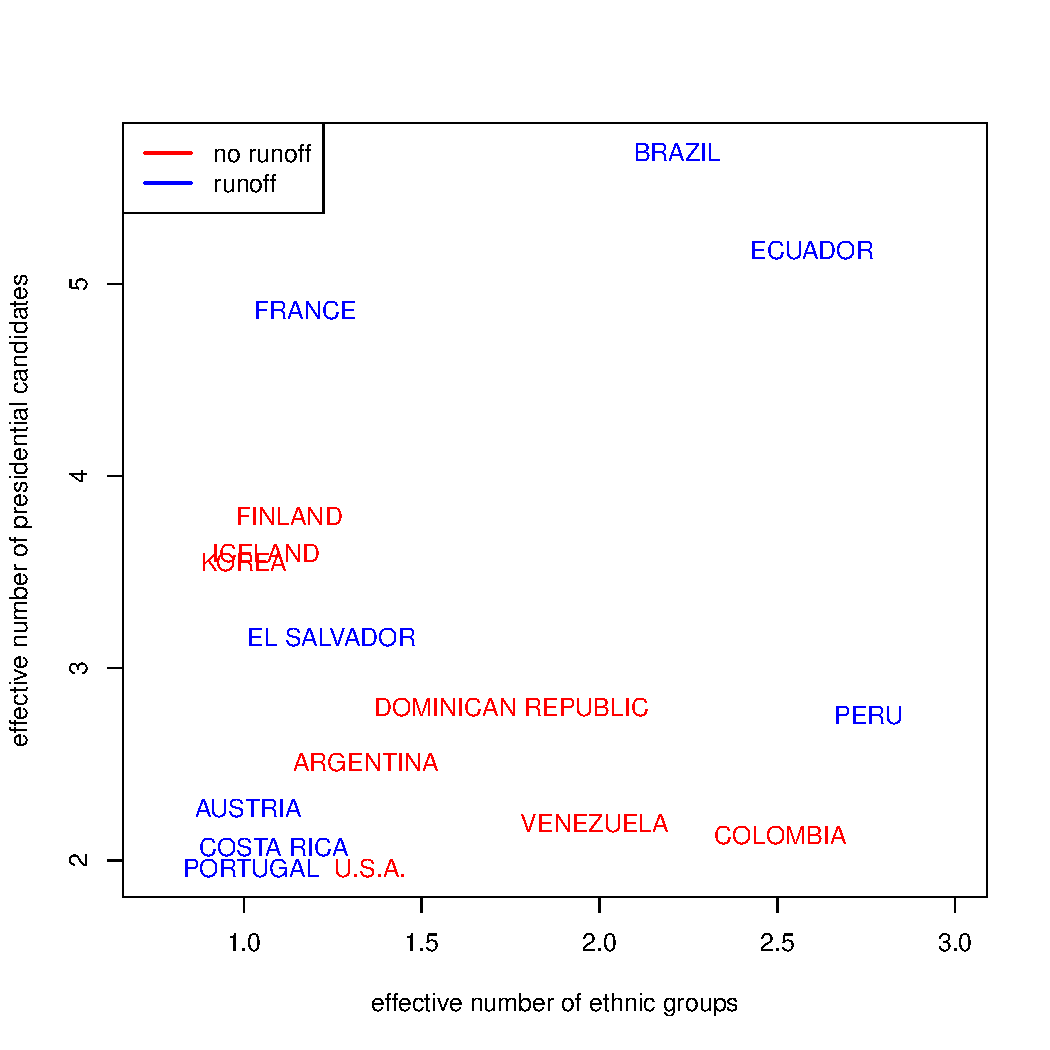
\includegraphics[height=3in]{figures/p1.pdf}
  \end{center}
  \vspace{-0.275in}
\end{figure}

}

\frame{
\frametitle{Average Partial Derivative (Runoff) in Additive Model}

\begin{figure}[ht]
  \begin{center}
    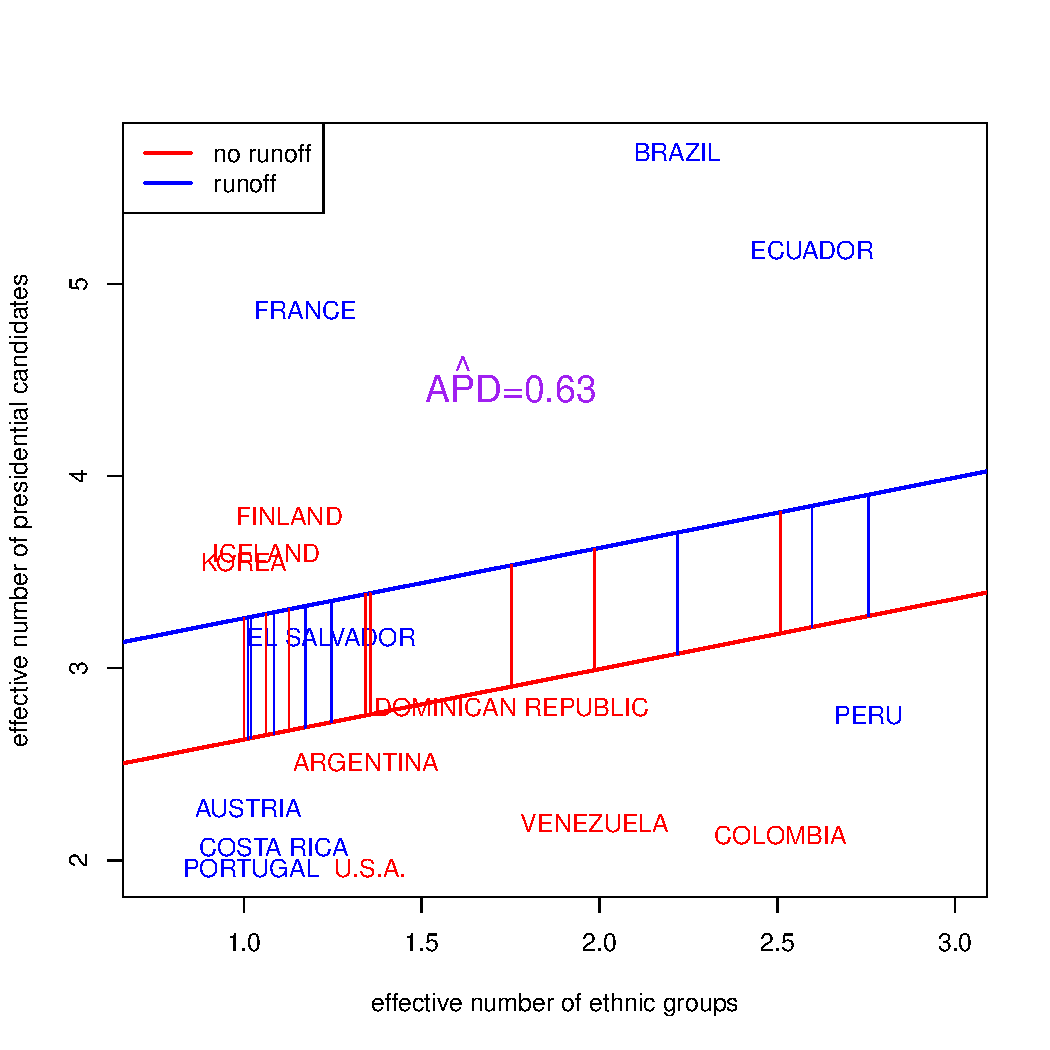
\includegraphics[height=3in]{figures/p2b.pdf}
  \end{center}
  \vspace{-0.275in}
\end{figure}

}

\frame{
\frametitle{APD in Interactive/Unpooled Linear Model}

\begin{figure}[ht]
  \begin{center}
    \includegraphics<1>[height=3in]{figures/p3.pdf}
    \includegraphics<2>[height=3in]{figures/p4b.pdf}
  \end{center}
  \vspace{-0.275in}
\end{figure}

}

\frame{
\frametitle{APD in Additive Quadratic Models}

\begin{figure}[ht]
  \begin{center}
    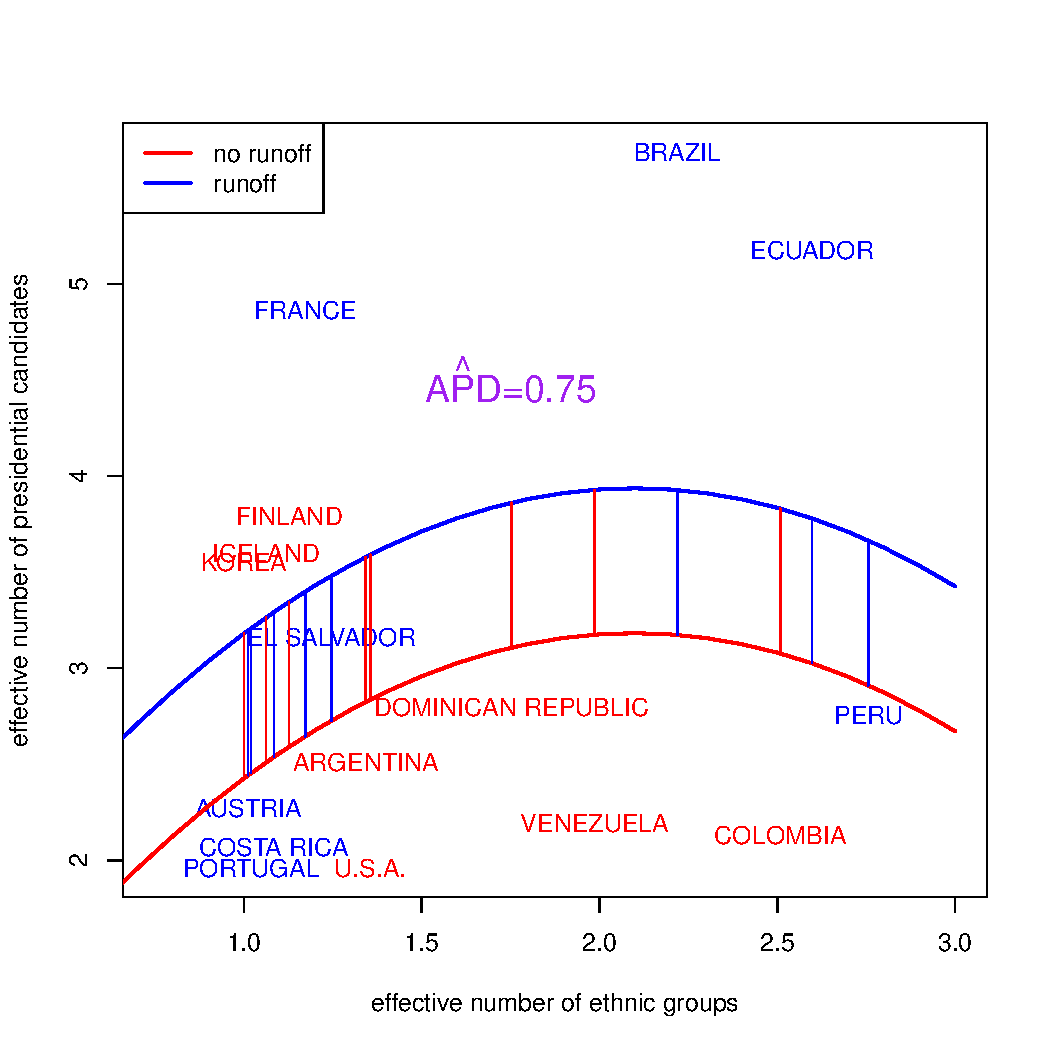
\includegraphics[height=3in]{figures/p13b.pdf}
  \end{center}
  \vspace{-0.275in}
\end{figure}

}


\frame{
\frametitle{APD in Interactive/Unpooled Quadratic}

\begin{figure}[ht]
  \begin{center}
    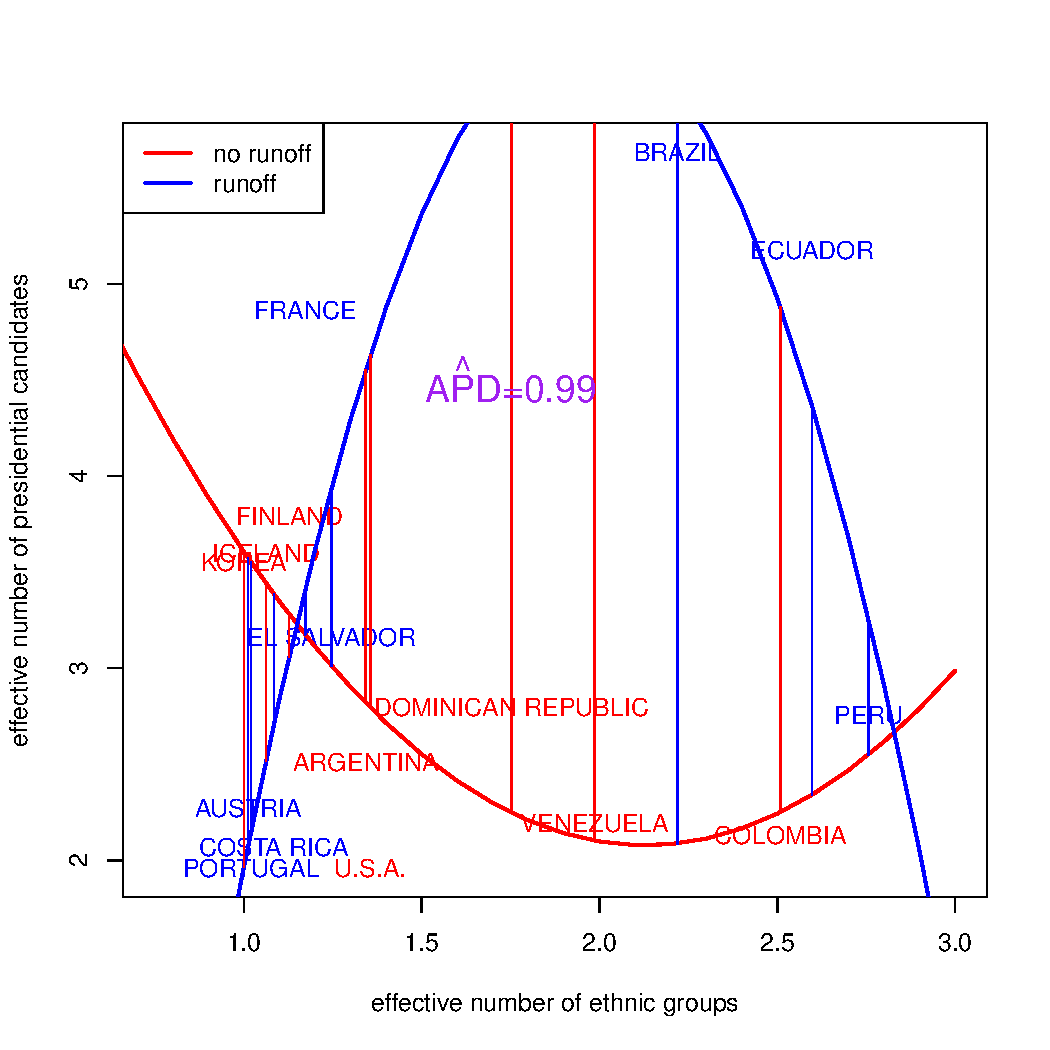
\includegraphics[height=3in]{figures/p13c.pdf}
  \end{center}
  \vspace{-0.275in}
\end{figure}

}

\frame{
\frametitle{APD in Unpooled Local Regression}

\begin{figure}[ht]
  \begin{center}
    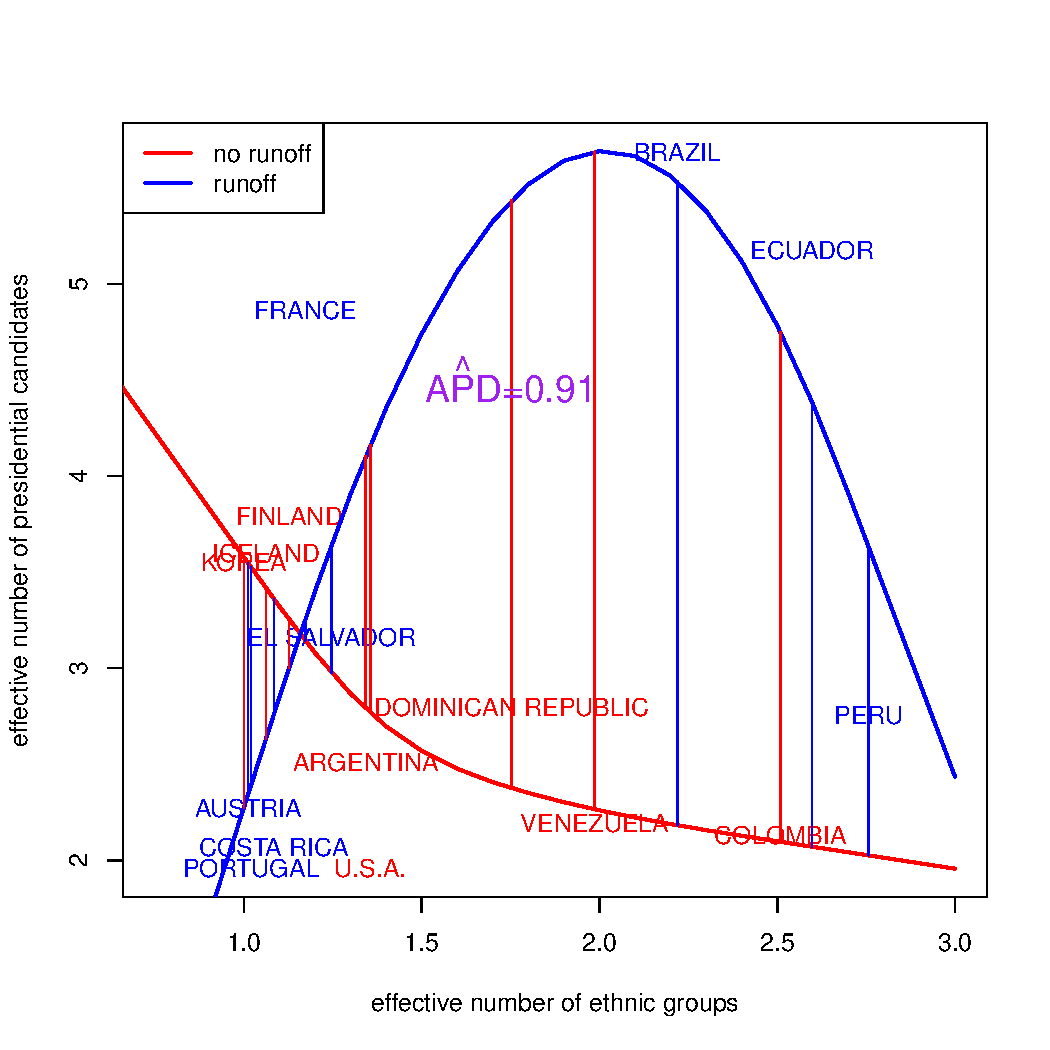
\includegraphics[height=3in]{figures/p15d.pdf}
  \end{center}
  \vspace{-0.275in}
\end{figure}

}




%\frame{
%\frametitle{Average Partial Derivative (Runoff) for the Runoff Countries}
%
%\begin{figure}[ht]
%  \begin{center}
%    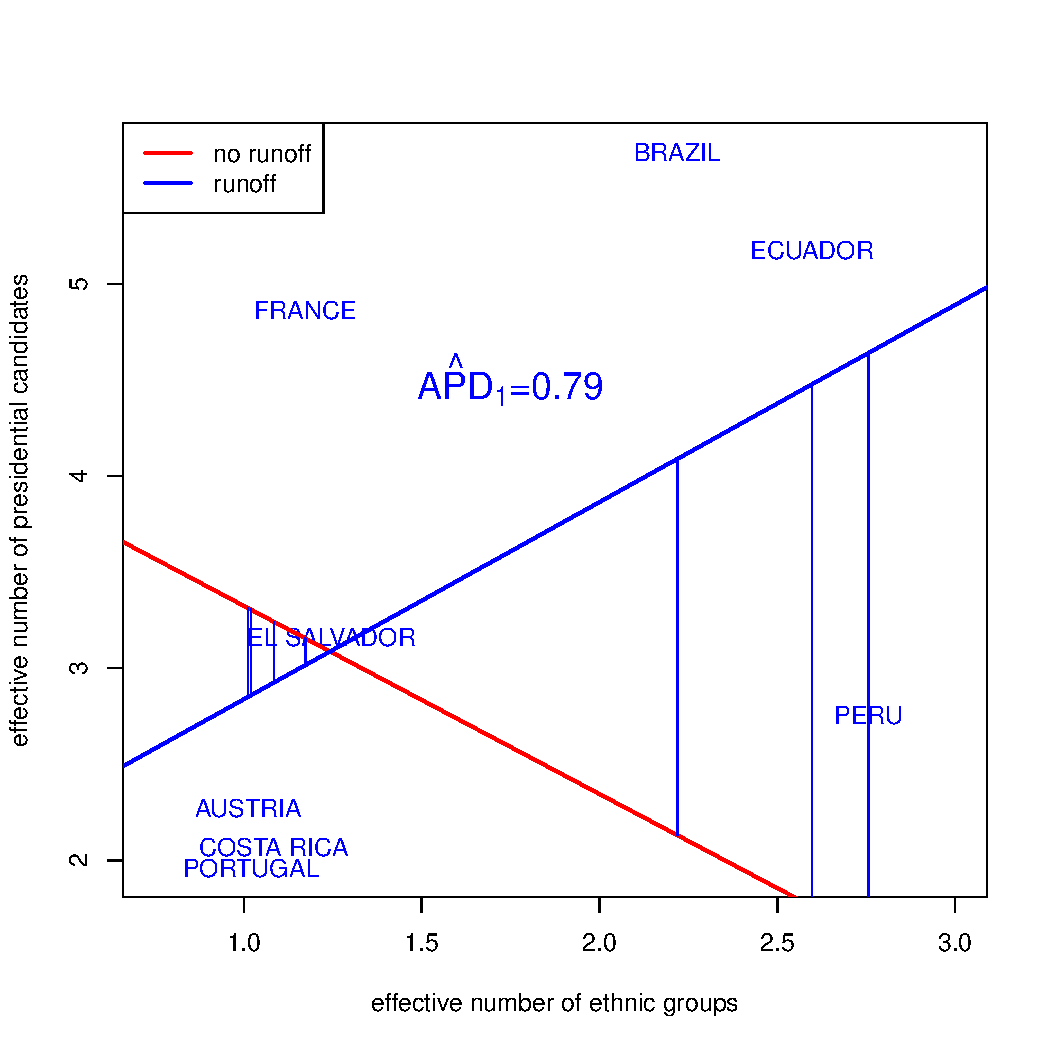
\includegraphics[height=3in]{figures/p5.pdf}
%  \end{center}
%  \vspace{-0.275in}
%\end{figure}
%
%}
%
%\frame{
%\frametitle{Average Partial Derivative (Runoff) for the Non-Runoff Countries}
%
%\begin{figure}[ht]
%  \begin{center}
%    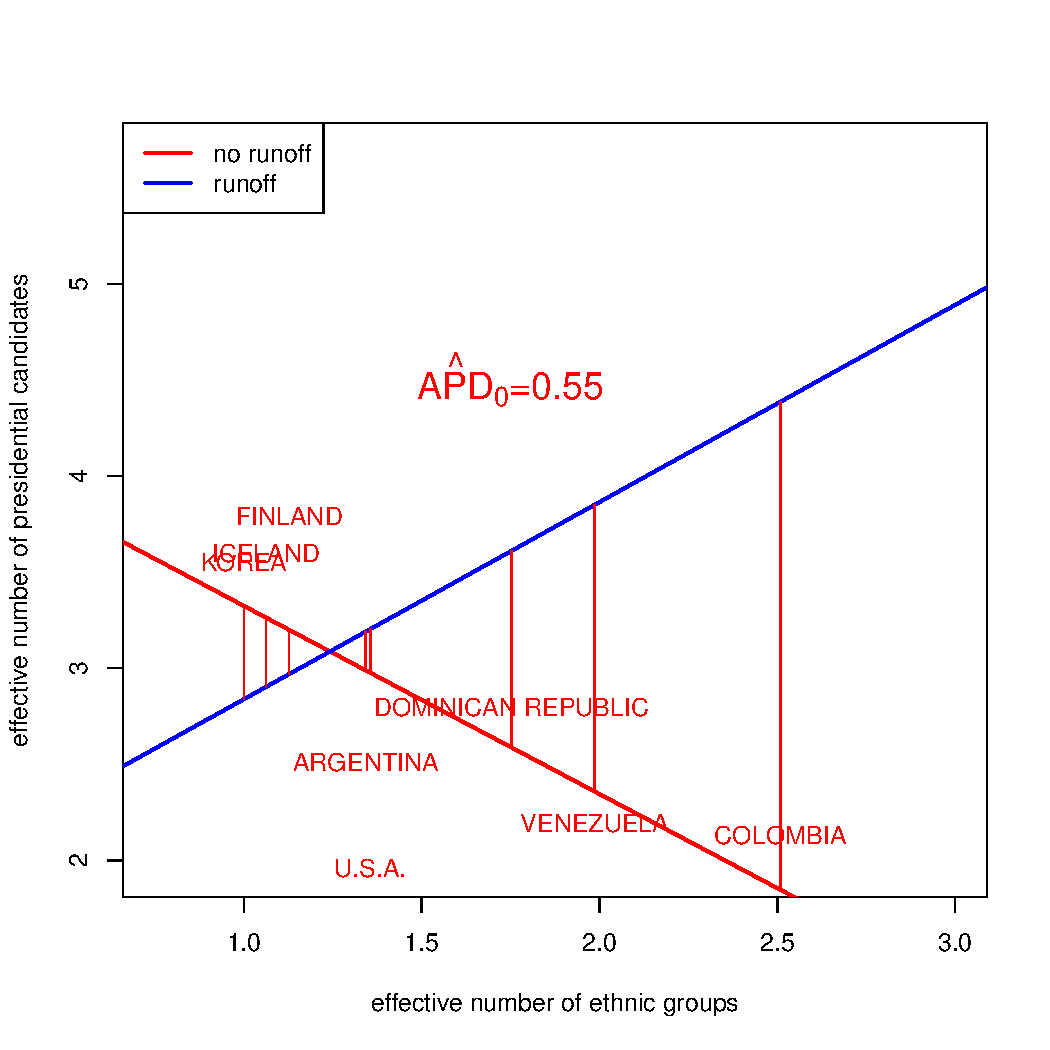
\includegraphics[height=3in]{figures/p6.pdf}
%  \end{center}
%  \vspace{-0.275in}
%\end{figure}
%
%}
%
%\frame{
%\frametitle{Imputation APD for  Non-Runoff Countries}
%
%\begin{figure}[ht]
%  \begin{center}
%    \includegraphics<1>[height=3in]{figures/p7.pdf}
%    \includegraphics<2>[height=3in]{figures/p8.pdf}
%    \includegraphics<3>[height=3in]{figures/p8b.pdf}
%  \end{center}
%  \vspace{-0.275in}
%\end{figure}
%
%}
%
%\frame{
%\frametitle{Imputation APD for  Non-Runoff Countries}
%
%\begin{figure}[ht]
%  \begin{center}
%    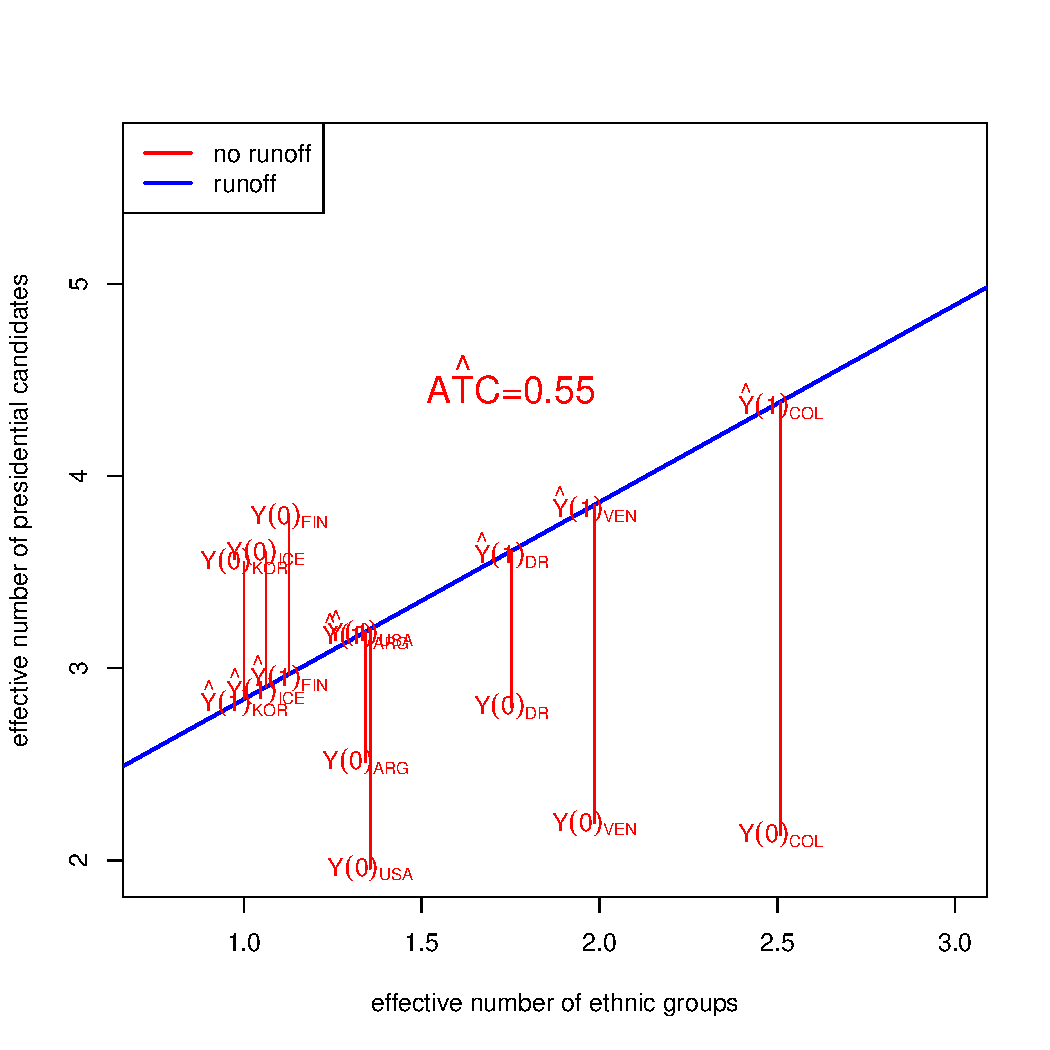
\includegraphics[height=3in]{figures/p9.pdf}
%  \end{center}
%  \vspace{-0.275in}
%\end{figure}
%
%}

%\frame{
%\frametitle{Diagnostics}
%
%\begin{figure}[ht]
%  \begin{center}
%    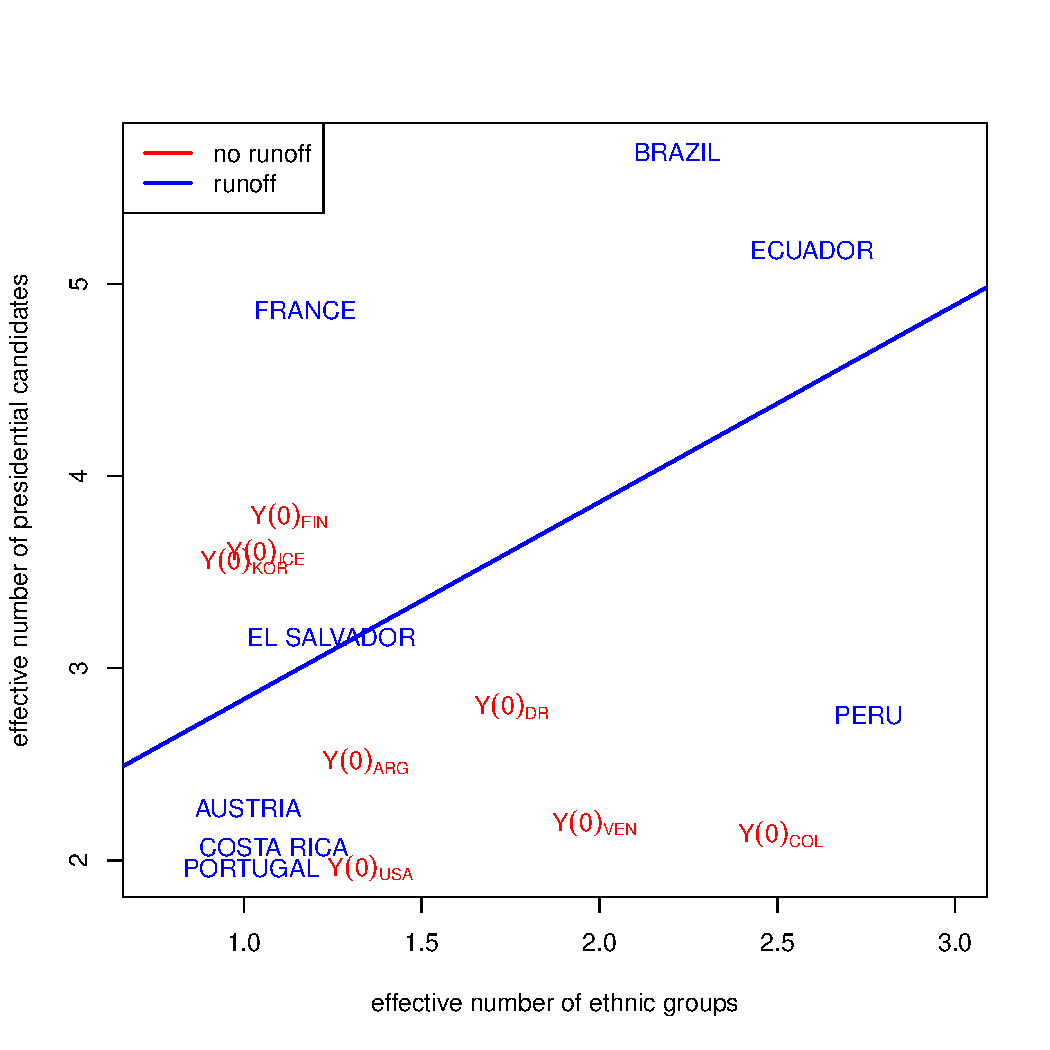
\includegraphics[height=3in]{figures/p10.pdf}
%  \end{center}
%  \vspace{-0.275in}
%\end{figure}
%
%}
%
%\frame{
%\frametitle{Balance and Overlap}
%
%\begin{figure}[ht]
%  \begin{center}
%    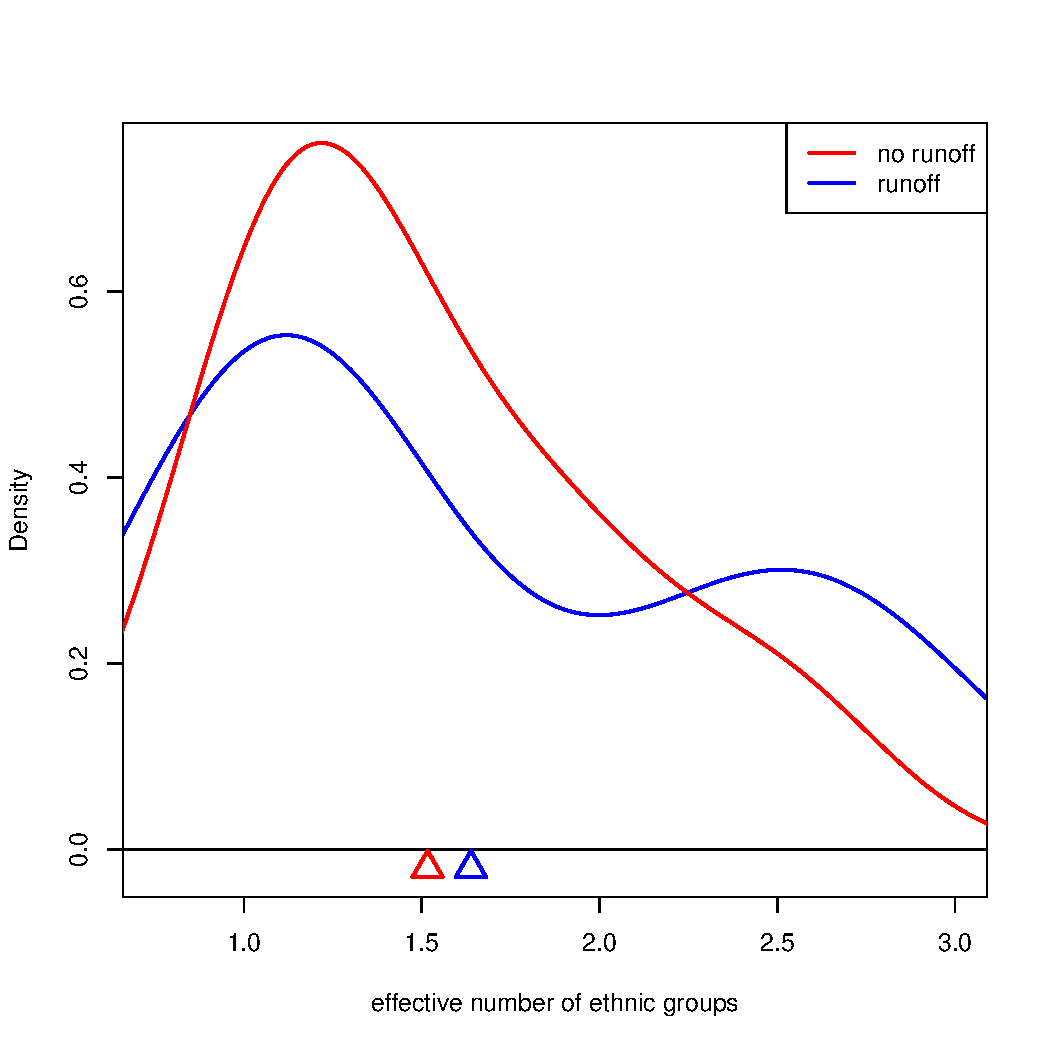
\includegraphics[height=3in]{figures/p11.pdf}
%  \end{center}
%  \vspace{-0.275in}
%\end{figure}
%
%}

%\frame{
%\frametitle{Nonlinearity (Quadratic)}
%
%\begin{figure}[ht]
%  \begin{center}
%    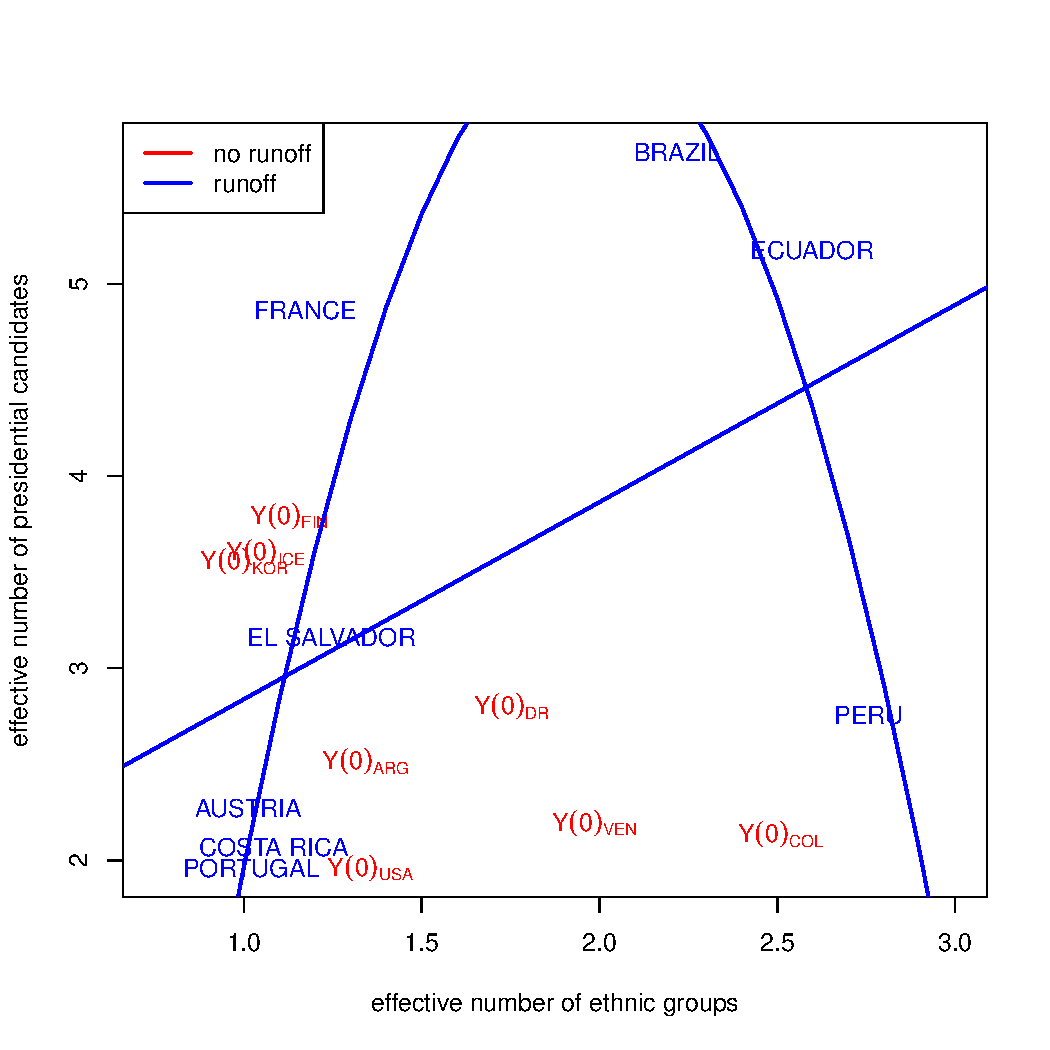
\includegraphics[height=3in]{figures/p12.pdf}
%  \end{center}
%  \vspace{-0.275in}
%\end{figure}
%
%}
%
%\frame{
%\frametitle{APD for Non-runoff Countries with Nonlinearity (Quadratic)}
%
%\begin{figure}[ht]
%  \begin{center}
%    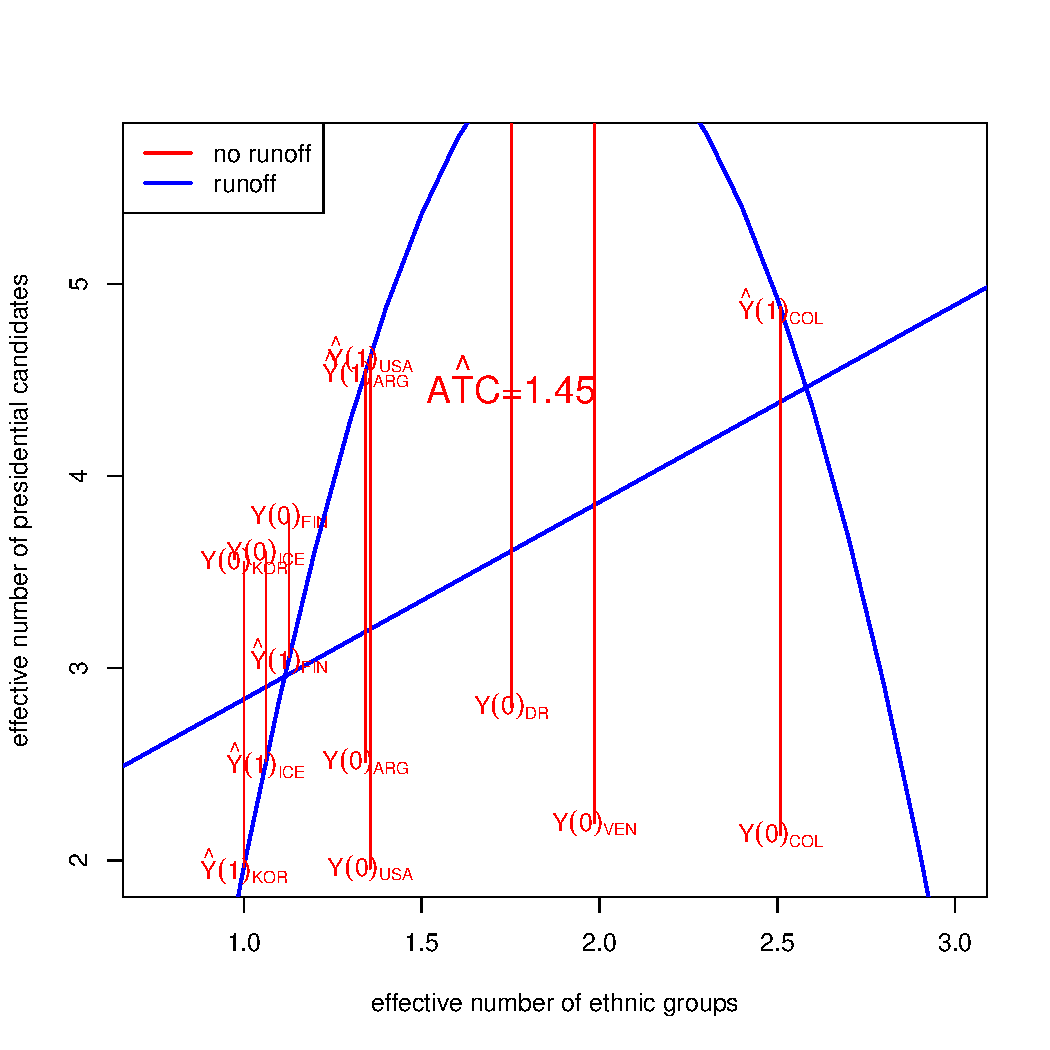
\includegraphics[height=3in]{figures/p13.pdf}
%  \end{center}
%  \vspace{-0.275in}
%\end{figure}
%
%}
%
%\frame{
%\frametitle{APD for Runoff Countries}
%
%\begin{figure}[ht]
%  \begin{center}
%    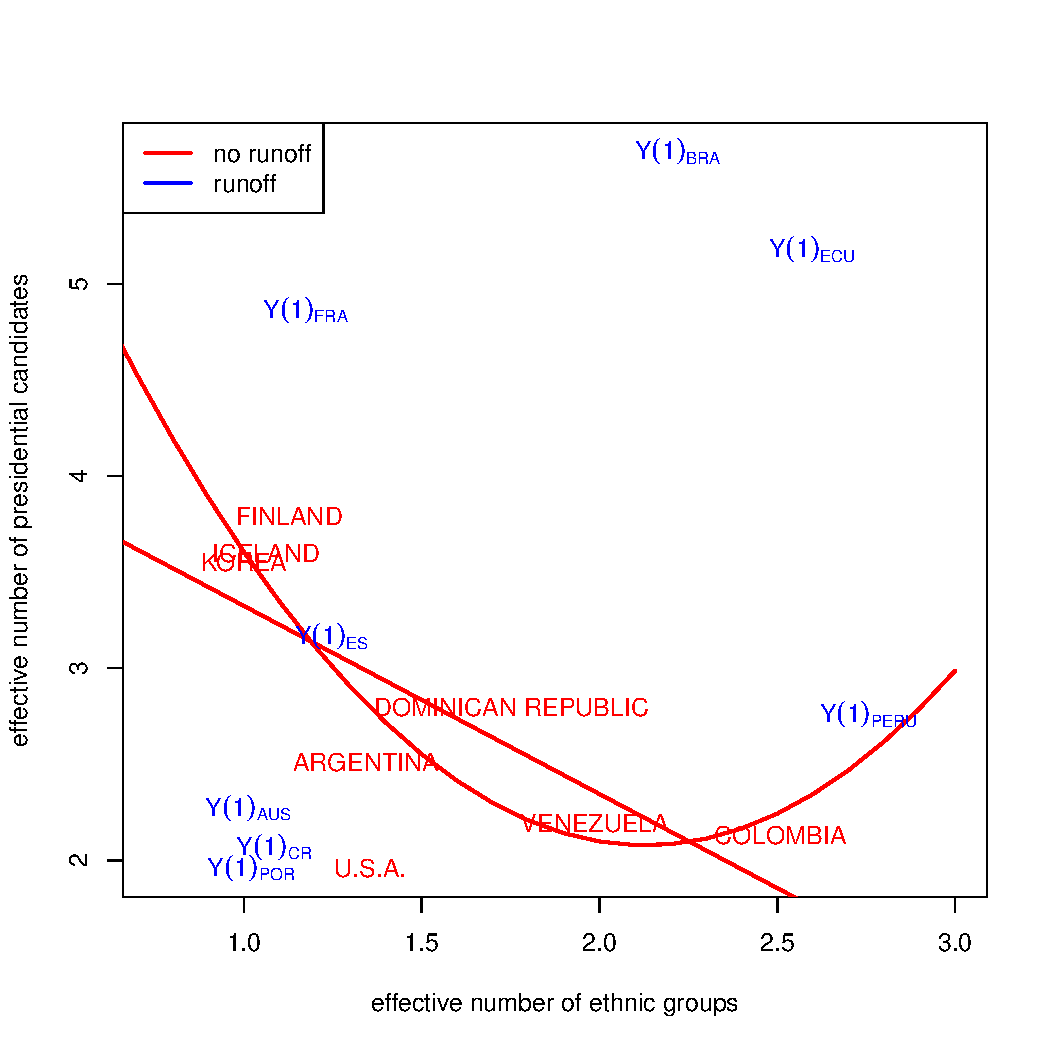
\includegraphics[height=3in]{figures/p14.pdf}
%  \end{center}
%  \vspace{-0.275in}
%\end{figure}
%
%}
%
%
%\frame{
%\frametitle{APD for Runoff Countries (Quadratic)}
%
%\begin{figure}[ht]
%  \begin{center}
%    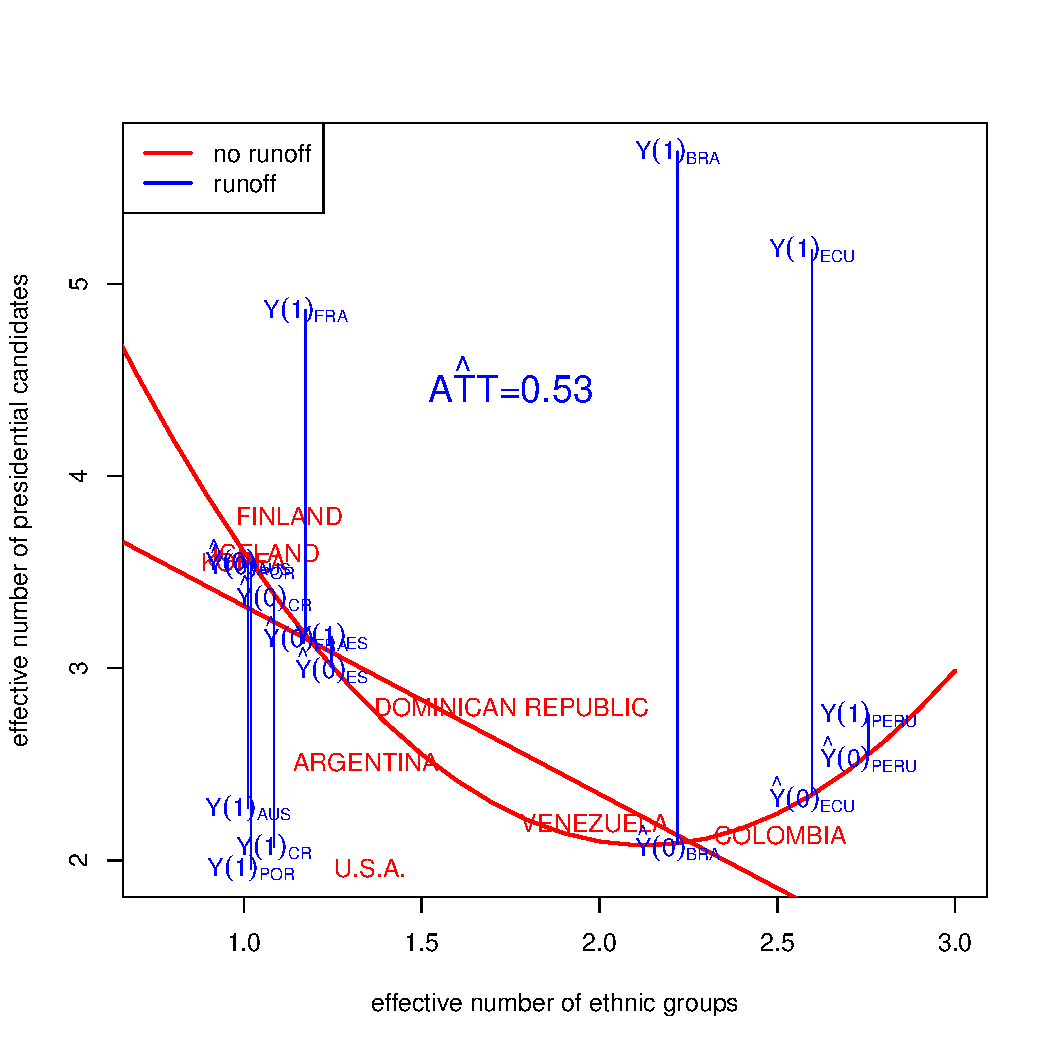
\includegraphics[height=3in]{figures/p15.pdf}
%  \end{center}
%  \vspace{-0.275in}
%\end{figure}
%
%}
%
%\frame{
%\frametitle{APD for Runoff Countries with Local Regression}
%
%\begin{figure}[ht]
%  \begin{center}
%    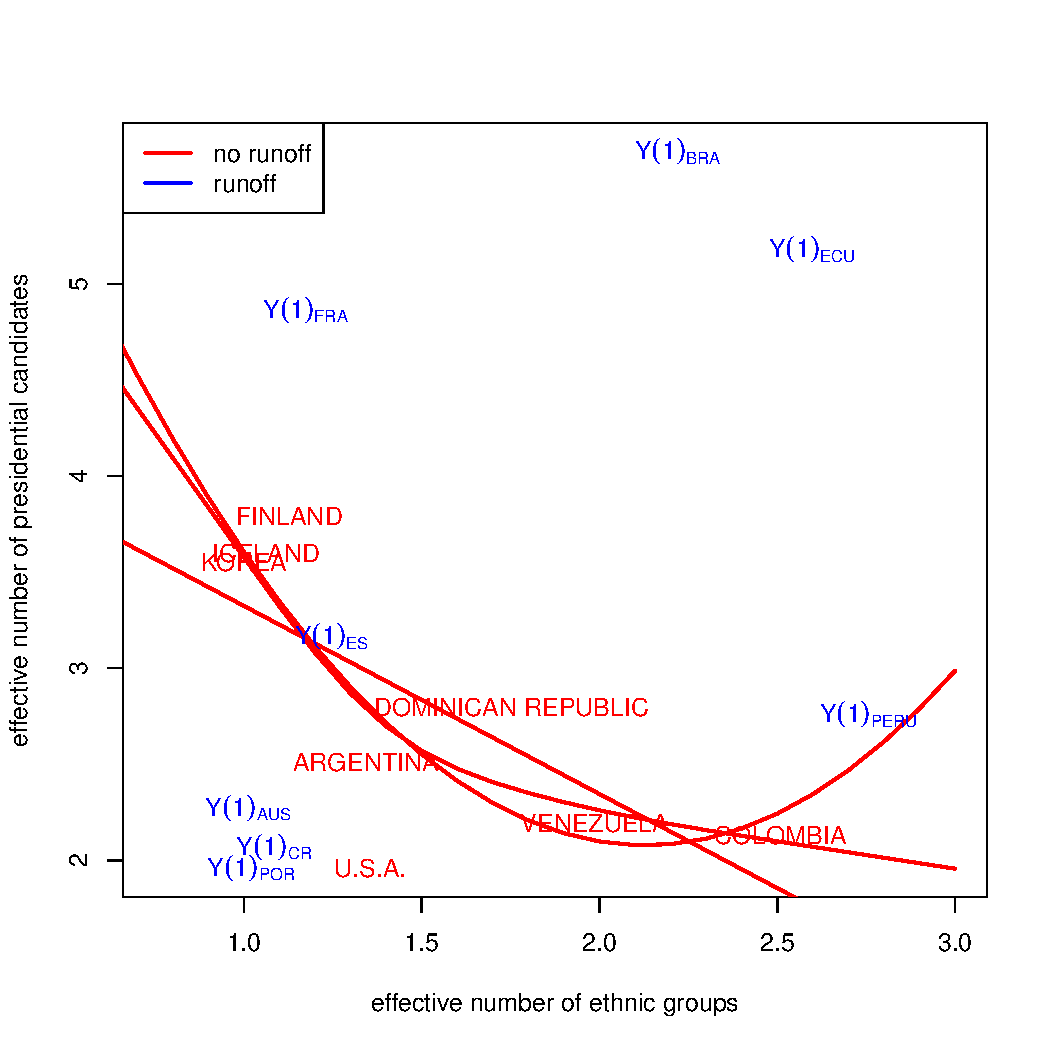
\includegraphics[height=3in]{figures/p15a.pdf}
%  \end{center}
%  \vspace{-0.275in}
%\end{figure}
%
%}
%
%
%\frame{
%\frametitle{APD for Runoff Countries with Local Regression}
%
%\begin{figure}[ht]
%  \begin{center}
%    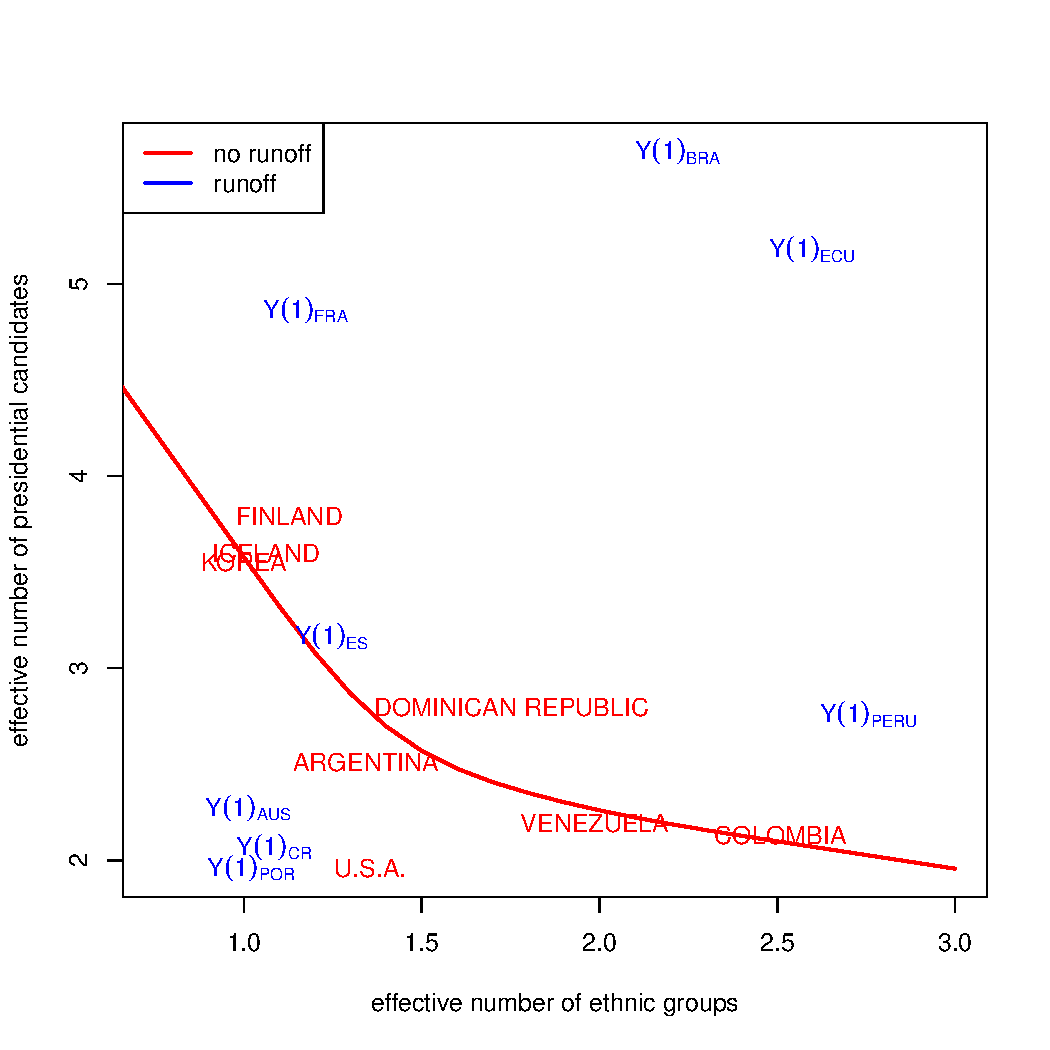
\includegraphics[height=3in]{figures/p15b.pdf}
%  \end{center}
%  \vspace{-0.275in}
%\end{figure}
%
%}
%
%
%\frame{
%\frametitle{APD for Runoff Countries with Local Regression}
%
%\begin{figure}[ht]
%  \begin{center}
%    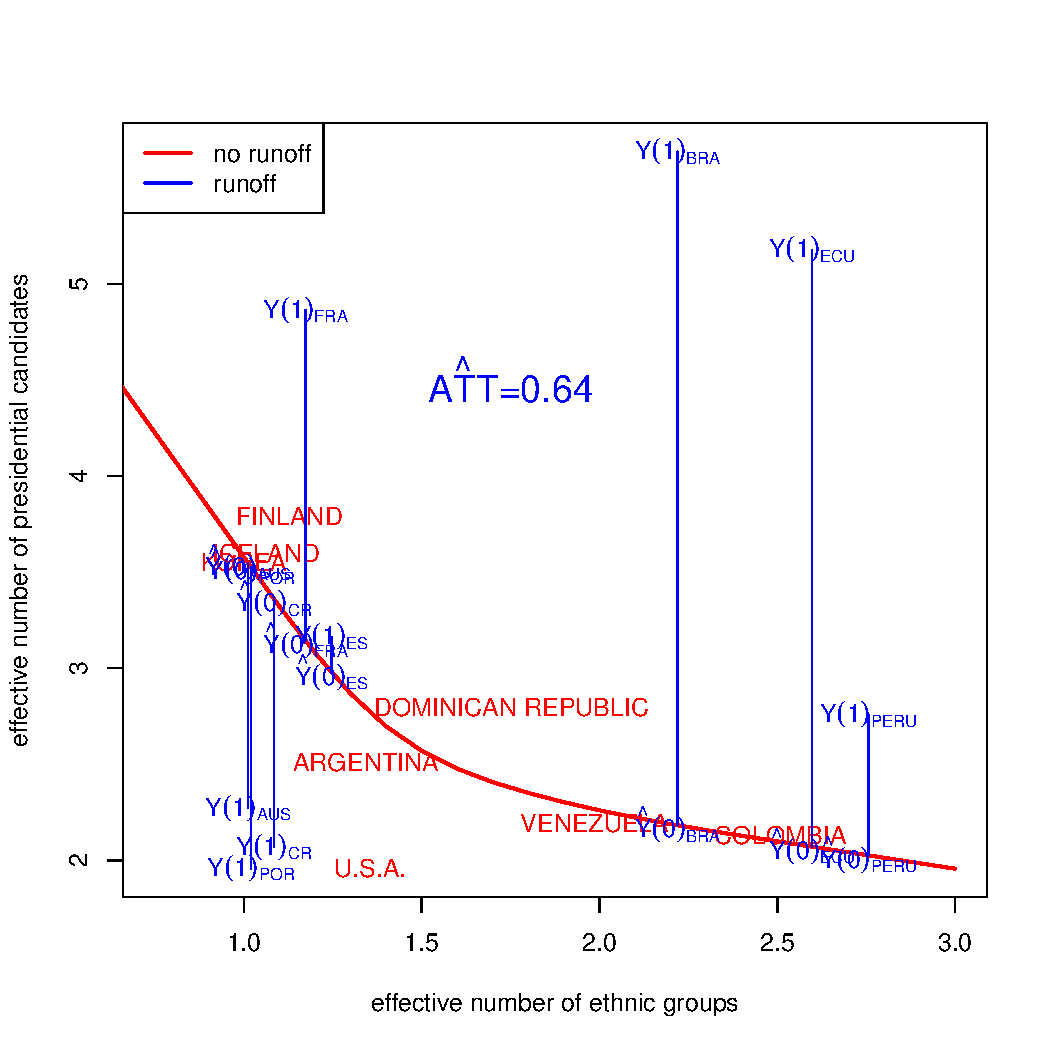
\includegraphics[height=3in]{figures/p15c.pdf}
%  \end{center}
%  \vspace{-0.275in}
%\end{figure}
%
%}
%








%\frame{
%
%Then considering the bivariate CEF, by definition:
%$$
%\E[Y| X = x] = \left\{
%     \begin{array}{lr}
%            \E[Y | X = 0]  & : x = 0 \\
%       \E[Y | X = 1] & : x = 1
%     \end{array}
%   \right.
%   $$
%
%}
%
%\frame{
%
%Then we can {\it definitionally} write $\E[Y| X]$ as a linear function of $X$.
%$$
%\E[Y| X] = \beta_0 + \beta_1 X,
%$$
%where
%\begin{itemize}
%\item $\beta_0 =  \E[Y | X = 0] $
%\item $\beta_1 =  \E[Y | X = 1] - \E[Y | X = 0]$.
%\end{itemize}
%
%}
%
%\frame{
%
%We could define an alternative specification that is logically equivalent. Consider the regression {\it without an intercept}:
%$$
%\E[Y| X] = \gamma_1(1 - X) + \gamma_2 X,
%$$
%where
%\begin{itemize}
%\item $\gamma_1 =  \E[Y | X = 0] $
%\item $\gamma_2 =  \E[Y | X = 1]$.
%\end{itemize}
%
%}
%
%\frame{
%
%When $X$ is binary, the CEF {\it must be} the BLP.
%
%\vspace{0.2in}
%
%The regression estimates of the $\beta$s can be written {\it just using} conditional means.
%
%}
%
%
%
%
%\frame{
%
%The idea generalizes to the multivariate case.
%
%}
%
%\frame{
%
%Consider binary $X_1$, $X_2$:
%
%$$
%\E[Y| X_1 = x_1, X_2 = x_2] = \left\{
%     \begin{array}{lr}
%            \E[Y | X_1 = 0, X_2 = 0]  & : x_1 = 0, x_2 = 0 \\
%            \E[Y | X_1 = 1, X_2 = 0]  & : x_1 = 1, x_2 = 0 \\
%            \E[Y | X_1 = 0, X_2 = 1]  & : x_1 = 0, x_2 = 1 \\
%            \E[Y | X_1 = 1, X_2 = 1]  & : x_1 = 1, x_2 = 1
%     \end{array}
%   \right.
%   $$
%
%}
%
%\frame{
%
%Then we can {\it definitionally} write $\E[Y| X_1, X_2]$ as a linear function of $X_1$, $X_2$ and $X_1 X_2$.
%
%$$
%\E[Y  | X_1, X_2] = \beta_0 + \beta_1 X_1 + \beta_2 X_2 + \beta_3 X_1 X_2
%$$
%where
%\begin{itemize}
%\item $\beta_0 =  \E[Y | X_1 = 0, X_2 = 0]  $
%\item $\beta_1 =   \E[Y | X_1 = 1, X_2 = 0]  -   \E[Y | X_1 = 0, X_2 = 0] $
%\item $\beta_2 =   \E[Y | X_1 = 0, X_2 = 1]  -   \E[Y | X_1 = 0, X_2 = 0] $
%\item $\beta_3 =   \E[Y | X_1 = 1, X_2 = 1]  - \E[Y | X_1 = 1, X_2 = 0]  - \E[Y | X_1 = 0, X_2 = 1] - \E[Y | X_1 = 0, X_2 = 0]$
%\end{itemize}
%
%}
%
%
%\frame{
%
%Logically equivalent, using indicator or ``dummy" variables:
%
%\begin{align*}
%\E[Y  | X_1, X_2]  = & \gamma_1 \I[X_1 = 0, X_2 = 0]  + \gamma_2 \I[X_1 = 1, X_2 = 0] +\\
%& \gamma_3 \I[X_1 = 0, X_2 = 1] + \gamma_4 \I[X_1 = 1, X_2 = 1]
%\end{align*}
%where
%\begin{itemize}
%\item $\gamma_1 =  \E[Y | X_1 = 0, X_2 = 0]  $
%\item $\gamma_2 =   \E[Y | X_1 = 1, X_2 = 0]  $
%\item $\gamma_3 =   \E[Y | X_1 = 0, X_2 = 1]  $
%\item $\gamma_4 =   \E[Y | X_1 = 1, X_2 = 1]  $
%\end{itemize}
%
%}
%
%\frame{
%
%These are cases of {\it saturated models}: when every unique combination of values of the explanatory variables is included in a fully flexible way. This is only possible with {\it discrete} regressors ($X$ variables).
%
%\vspace{0.2in}
%
%This means including dummy variables for every possible value of each variable, and all possible (including multiway) interactions. Or just dummy variables for each unique combination, and excluding the intercept.
%
%\vspace{0.2in}
%
%With a saturated model, the CEF is, by definition, the BLP.
%
%}
%
%
%
%
%
%
%\frame{
%
%Remaining ``non-linear'' issues with a single $X$:
%\begin{itemize}
%\item How to choose the degree of the polynomial?
%\item What if not linear in $\beta$?
%\item statistical/machine learning approaches
%\item what if $X$ is ordinal?
%\end{itemize}
%
%}

%\frame{
%How to choose the degree of the polynomial?
%\begin{itemize}
%\item Sieve Estimation:\\
%Choose the degree of the polynomial to be $K_n = \ceil{n^{1/9}}$
%\item Cross-validation:\\
%\begin{enumerate}
%\item Separate data into $G$ groups
%\item Leave one group out as test data
%\item fit model using remaining groups
%\item calculate prediction error on test data
%\item repeat for all $G$ groups
%\item repeat whole process for many different polynomials and choose best based on test data prediction error
%\end{enumerate}
%\end{itemize}
%
%}
%
%\frame{
%Leave one out CV
%
%\begin{itemize}
%\item $G=n$ (each observation is a group)
%\item test error easy to calculate for OLS (includes polynomial models)
%$$
%\frac{1}{n}\sum_{i=1}^n\frac{(y_i - \hat y_i)^2}{(1-h_i)^2}
%$$
%\end{itemize}
%
%}
%
%\frame{
%
%Examples of nonlinear in $\beta$
%
%\begin{align*}
%g(X) &= e^{\beta_0 + \beta_1 X}\\
%g(X) &= \frac{e^{\beta_0 + \beta_1 X}}{1 + e^{\beta_0 + \beta_1 X}}
%\end{align*}
%
%How to fit?
%
%\vsf
%
%How to interpret?
%%$$\frac{\partial g(X)}{\partial X} = ?$$
%
%}







\frame{

Local Regression 

\bi
\item Moving averages (on board)
\item go to JWHT ISL book pg. 305
\ei

}


%\frame{
%%\frametitle{Sampling}
%
%Why study sampling
%\begin{enumerate}
%\item<2-> model based i.i.d. not always a good approach for inferences from sample to population
%\item<3-> taking a random sample and then randomizing into treatment and control can be thought of as taking a random sample of treated units and a random sample of control units (i.e., causal inference with a binary treatment be thought of as two sampling problems)
%\item<4-> finite population sampling theory is the foundation of modern causal inference
%\begin{itemize}
%\item fixed outcomes (like potential outcomes)
%\item we often have a finite population (e.g., states)
%\item simplifies the interpretation of weighting approaches
%\item omitted variable problem like analyzing a stratified random sample as a SRS
%\end{itemize}
%\end{enumerate}
%
%
%}

%\frame{
%\frametitle{SRS vs Stratified}
%
%Suppose stratified sample of men and women with sampling probabilities $\pi_m$ and $\pi_w$ to estimate average height in population, but we analyze it as an SRS. What happens and how does it depend on  $\pi_m$ and $\pi_w$?
%
%}
%
%\frame{
%\frametitle{How to adjust?}
%
%
%
%How to adjust with weights? \pause
%
%
%How to adjust with regression?
%
%}


\frame{
\frametitle{Missing Data (Ch. 6 of AM)}

Let's start by considering a simple but common problem: missing data.

\vspace{0.2in}

What can we learn about the distribution of a variable of interest when some values are missing from, e.g., nonresponse.

\vspace{0.2in}

E.g., if we ran a survey asking people who they voted for, some people might not respond to the vote choice question. We want to know the population distribution of outcomes to the question, but we don't observe the answers for some people.

}


%\frame{
%Suppose that we were interested in estimating the expected value and/or full distribution of some random variable characterized by the distribution of $Y_i$. However, we {\it do not} observe $Y_i$ for any units such that units do not respond.
%
%\vspace{0.2in}
%
%We will primarily focus on {\it identification} results -- results assuming that we knew the joint distribution of all observable data, and that nothing needs to be estimated. Given i.i.d. sampling, then estimation proceeds via simple plug-in estimation (using sample analogues to population quantities).
%
%}
%
%\frame{
%
%Suppose that we had knowledge of the full joint distribution of a random vector generated by sampling values of $(Y_i^*, R_i)$.
%
%\vspace{0.2in}
%
%$R_i$ denotes whether or not unit $i$ has data available on $Y_i$ (i.e., unit $i$ responded), and $Y_i^*$ is a censored version of $Y_i$:
%$$
%Y_i^* = Y_i \cdot R_i + (-99) \cdot (1 - R_i)
%$$
%
%\vspace{0.2in}
%
%(This embeds an often-overlooked assumption of stable outcomes -- the underlying $Y_i$ for unit $i$ is {\it stable} and it does not depend on how you asked, who you asked or who responded. More on this later.)
%
%\vspace{0.2in}
%
%Suppose that our inferential target is then the expected value of $Y_i$, $\E[Y_i]$, which cannot be directly observed. Then the question is: what assumptions yield what information about $\E[Y_i]$?
%
%}

\frame{

Let's start with a minimal assumption. Without much loss of generality, suppose that $\Supp[Y_i] \subset [0,1]$. (For any bounded outcome variable, we could rescale to $[0,1]$.)

\vspace{0.2in}

With this assumption, we can derive {\it sharp bounds} (bounds that cannot be improved upon without further assumptions) on $\E[Y_i]$.

\vspace{0.2in}

These bounds are a special case of Manski bounds. See, e.g., Manski (2003).

}

\frame{

Manski bounds proceed by imputing the worst-case scenario for all missing data.

\vspace{0.2in}

For an upper bound, assume that all missing $Y_i$s are a 1. For a lower bound, assume that all missing $Y_i$s are 0.

}

\frame{

For example, we might see the following data:

\begin{table}
\begin{tabular}{ccc}
Unit & $Y_i^*$ & $R_i$ \\
1 & 1 & 1 \\
2 & -99 & 0\\
3 & 1 & 1 \\
4 & 0 & 1\\
5 & 1 & 1\\
6 & -99 & 0
\end{tabular}
\end{table}

}

\frame{


\begin{table}
\begin{tabular}{cccccccc}
Unit & $Y_i^*$ & $R_i$ & \hspace{0.5in} & Unit & $Y_i$ & $R_i$\\
1 & 1 & 1 && 1 & 1 & 1 \\
2 & -99 & 0 && 2 & {\color{blue} ?} & 0 \\
3 & 1 & 1 && 3 & 1 & 1 \\
4 & 0 & 1 && 4 & 0 & 1 \\
5 & 1 & 1 && 5 & 1 & 1 \\
6 & -99 & 0 && 6 & {\color{blue} ?} & 0
\end{tabular}
\end{table}

For units 2 and 6, we only know that $\Supp[Y_i] \subset [0,1]$.

}

\frame{
Using the sample mean as a plug-in estimator for the expected value, our estimate of a lower bound for $\E[Y_i]$:

\begin{table}
\begin{tabular}{cccccccc}
Unit & $Y_i^*$ & $R_i$ & \hspace{0.5in} & Unit & $Y_i$ & $R_i$\\
1 & 1 & 1 && 1 & 1 & 1 \\
2 & -99 & 0 && 2 & {\color{red}0} & 0 \\
3 & 1 & 1 && 3 & 1 & 1 \\
4 & 0 & 1 && 4 & 0 & 1 \\
5 & 1 & 1 && 5 & 1 & 1 \\
6 & -99 & 0 && 6 & {\color{red}0} & 0
\end{tabular}
\end{table}

Estimated lower bound for $\E[Y_i]$ is 1/2.

}

\frame{
Using the sample mean as a plug-in estimator for the expected value, our estimate of a upper bound for $\E[Y_i]$:

\begin{table}
\begin{tabular}{cccccccc}
Unit & $Y_i^*$ & $R_i$ & \hspace{0.5in} & Unit & $Y_i$ & $R_i$\\
1 & 1 & 1 && 1 & 1 & 1 \\
2 & -99 & 0 && 2 & {\color{red}1} & 0 \\
3 & 1 & 1 && 3 & 1 & 1 \\
4 & 0 & 1 && 4 & 0 & 1 \\
5 & 1 & 1 && 5 & 1 & 1 \\
6 & -99 & 0 && 6 & {\color{red}1} & 0
\end{tabular}
\end{table}

Estimated upper bound for $\E[Y_i]$ is 5/6.

}

\frame{

Go to QoGmissing.R

}

\frame{

Ch. 7 of AM will be in different slides. 

}

\end{document}